\documentclass[12pt, a4paper]{report}

%dvips
\usepackage[pdftex, pdfauthor={Yan King Yin}, bookmarks, anchorcolor=blue, colorlinks, linkcolor=blue, citecolor=blue, urlcolor=blue, breaklinks, plainpages=false, pdfpagelabels, hypertexnames=false]{hyperref}
\usepackage{breakurl}
\usepackage[final]{graphicx}
\usepackage{float}
\usepackage[square]{natbib}
\usepackage{color}
\usepackage{amsmath}   % for {equation} {cases} {xleftarrow}
\usepackage{bbm}         % for math fonts with double lines
\usepackage{amssymb}   % for \curlyvee
\usepackage{stmaryrd}   % for \bigcurlyvee, \widetilde{\bigwedge}
\usepackage{wasysym}   % for \iint (double integral)
\usepackage{makeidx}
\usepackage[style=list,acronym=true,number=none]{glossary}
\usepackage{alg}
\usepackage{minitoc}
\usepackage[pointedenum]{paralist}
\usepackage[sf,bf,big,raggedright,compact]{titlesec}
\usepackage{fancyhdr}
\usepackage{movie15}
\usepackage{caption}

\definecolor{DarkGreen}{rgb}{0.1,0.4,0.1}

\newcommand{\code}[1]{{\footnotesize{\ttfamily #1}}}
\newcommand{\formula}[1]{\textcolor{DarkGreen}{#1}}
\renewcommand{\star}{$* \;$}
\newcommand{\app}{$\cdot \;$}
\newcommand{\eg}{\textbf{Example:} }
\newcommand{\tab}{\hspace*{1cm} }
\newcommand{\underconst}{
\includegraphics{UnderConst.png}}
\renewcommand{\vec}[1]{\mathbf{#1}}

%%%%%%%%%%%%%%%%% Symbols defined by me %%%%%%%%%%%%%%%%%%%
% fuzzy and probabilistic logic operators
\newcommand{\Zand}{\stackrel{Z}{\wedge}}
\newcommand{\Zor}{\stackrel{Z}{\vee}}
\newcommand{\Pand}{\stackrel{P}{\wedge}}
\newcommand{\Por}{\stackrel{P}{\vee}}
\newcommand{\bigZand}{\stackrel{Z}{\bigwedge}}
\newcommand{\bigZor}{\stackrel{Z}{\bigvee}}
\newcommand{\bigPand}{\stackrel{P}{\bigwedge}}
\newcommand{\bigPor}{\stackrel{P}{\bigvee}}
\newcommand{\Pimp}{\rightarrowtriangle}
% categories
\newcommand{\catP}{\mathcal{P}}
\newcommand{\catZ}{\mathcal{Z}}
\newcommand{\catB}{\mathcal{B}}
\newcommand{\catPB}{\mathcal{P(B)}}
\newcommand{\catPZ}{\mathcal{P(Z)}}

\fontsize{13pt}{15pt} \selectfont
\renewcommand{\familydefault}{\sfdefault}
%\renewcommand{\mtcfont}{\small\sffamily}
%\renewcommand{\mtcSfont}{\small\sffamily}
%\renewcommand{\mtcSSfont}{\small\sffamily}
%\renewcommand{\mtcSSSfont}{\small\sffamily}
%\renewcommand{\mtifont}{\small\sffamily}
\renewcommand{\mtcfont}{\normalsize\sffamily}
\renewcommand{\mtcSfont}{\normalsize\sffamily}
\renewcommand{\mtcSSfont}{\normalsize\sffamily}
\renewcommand{\mtcSSSfont}{\normalsize\sffamily}
\renewcommand{\mtifont}{\normalsize\sffamily}
%\renewcommand{\mtcfont}{\large\sffamily}
%\renewcommand{\mtcSfont}{\large\sffamily}
%\renewcommand{\mtcSSfont}{\large\sffamily}
%\renewcommand{\mtcSSSfont}{\large\sffamily}
%\renewcommand{\mtifont}{\large\sffamily}
\renewcommand{\mtctitle}{}
\renewcommand{\chaptername}{Ch }

\titlespacing{\chapter}{0pt}{0pt}{0pt}
\titleformat{\chapter}[hang]{\sffamily\bfseries\Huge\color{blue}}{\thechapter \hspace{30pt}}{0pt}{}
\titleformat{\appendix}[hang]{\sffamily\bfseries\Huge\color{blue}}{\thechapter \hspace{30pt}}{0pt}{}
\titleformat{\section}[hang]{\sffamily\bfseries\Large\color{blue}}{\thesection \hspace{10pt}}{0pt}{}
\titleformat{\subsection}[hang]{\sffamily\bfseries\large\color{blue}}{\thesubsection \hspace{5pt}}{0pt}{}
\titleformat{\subsubsection}[hang]{\sffamily\bfseries\color{blue}}{\thesubsubsection \hspace{5pt}}{0pt}{}

\newcommand{\algrepeatforever}{\textbf{repeat forever}\\\algbegin}

\interfootnotelinepenalty=50000

\title{\textbf{Genifer\\-- an artificial general intelligence}}
\author{Yan King Yin (general.intelligence@Gmail.com)\\ \\
with input from:\\
Abram Demski\\
Ben Goertzel\\
Martin Magnusson\\
Russell Wallace\\
Pei Wang
}
\date{\copyright \quad latest revision: \today}

\setlength{\headheight}{0cm}
\setlength{\hoffset}{0cm}
\setlength{\topmargin}{0cm}
\setlength{\oddsidemargin}{-2cm}
\setlength{\evensidemargin}{-2cm}
\setlength{\textwidth}{19.5cm}
\setlength{\textheight}{26cm}
\setlength{\headsep}{0cm}
\setlength{\topskip}{0cm}
\setlength{\footskip}{0.9cm}  % between bottom of page and page number
\setlength{\floatsep}{0cm}
\setlength{\textfloatsep}{0.6cm}
\setlength{\intextsep}{0.5cm}
\setlength{\parindent}{0em}
\setlength{\parskip}{7pt}
\setlength{\pltopsep}{-5pt}   % for compact-enum

\pagestyle{fancy}
\renewcommand{\headrulewidth}{0pt}
\rhead{}
\lhead{}
\cfoot{}
\rfoot{\thepage}
\fancypagestyle{plain}{\rfoot{\thepage}}
%\pagestyle{plain}

\includeonly{introduction, architecture, knowledge-representation, logic, vagueness, probabilities, confidence, inference, pattern-recognition, belief-revision, induction, natural-language, memory-systems, planning, program-synthesis, value-judgements, vision, implementation, business-aspects, quick-start, symbols}

\makeindex
\makeglossary

\begin{document}
%\font\normalfont=cmss14
\renewcommand{\normalsize}{\fontsize{13pt}{15pt}\selectfont}
\fontsize{13pt}{15pt} \selectfont

%\pagestyle{plain}
%\newcommand\ps@plain{
%\renewcommand\@oddhead{}
%\let\@evenhead\@oddhead
%\renewcommand\@evenfoot
%    {\hfil{\thepage}}
%\let\@oddfoot\@evenfoot
%}

\maketitle
\dominitoc
\tableofcontents

\setcounter{chapter}{-1}
\chapter{Preface}

\begin{enumerate}

\item  This book is a perpetual draft.  Some people get upset that it is very unpolished and contains ideas that I often retract later.  I find the pros of doing this out-weight the cons:  It allows us to develop our theory much more rapidly.  Very often the details I glossed over are superceded by higher-level design changes and the previous details recede to much lesser importance.  The con is that this book may not be up to scholarly standards.

\item  My \textit{personal} top priority is to obtain life extension if and when the technology is available.  I guess:\\
\hspace*{1cm} if sufficiently many people want technology X,\\
\hspace*{1cm} and X can be achieved at a cost affordable by those people,\\
\hspace*{1cm} then X is likely to happen.\\
I estimate my natural death would be around 2048, so for me AGI must happen before 2023, to allow 25 years of AGI diffusion (just to be safe!)  That means I have $\sim$13 years to build an AGI.  I don't mean to sound selfish, this is just to let people understand my priorities and motives better.

\item  The source code of $\mbox{Genifer}$ is hosted on \href{http://code.google.com/p/genifer/}{Google Code}, including some very nice \href{http://code.google.com/p/genifer/downloads/list}{tutorial slides}.  Also feel free to \href{mailto:Generic.Intelligence@Gmail.com}{contact me}!

\end{enumerate}

\begin{flushright}
--- YKY
\end{flushright}

\chapter{Introduction}
\begin{flushright}
\emph{I am an enthusiast, but not a crank in the sense that I have some\\
pet theories as to the proper construction of a flying machine. I wish to\\
avail myself of all that is already known and then, if possible,\\
add my mite to help on the future worker who will attain final success.}\\
--- Wilbur Wright
\end{flushright}

\begin{flushright}
\emph{Everything should be made as simple as possible, but no simpler.}\\
--- Albert Einstein (rephrased)
\end{flushright}

\begin{flushright}
\emph{An inventor is simply a fellow who doesn't take his education too seriously.}\\
--- Charles Kettering 
\end{flushright}

\begin{flushright}
\emph{When a subject becomes totally obsolete we make it a required course.}\\
--- Peter Drucker
\end{flushright}

%\begin{flushright}
%\emph{A problem well stated is a problem half-solved.}\\
%--- Charles Kettering
%\end{flushright}
\minitoc

This book describes a theory of AGI (Artificial General Intelligence) \citep*{Goertzel2007} that is still being developed.  I think the AGI problem can be decomposed into $\sim$10 computational issues and we will somehow integrate them together:

\leftskip 1cm
knowledge representation\\
fuzzy-probabilistic logic\\
deduction\\
abductive reasoning\\
inductive learning\\
pattern recognition / categorization\\
belief revision\\
memory organization\\
natural language\\
sensory processing

\leftskip 0cm
My approach is predominantly logic-based, but it also employs redundancy in knowledge representation, including sub-symbolic knowledge, and therefore is somewhat like neural networks.  Also, it may merge with neural networks at the sensory level.  This approach can be called ``neo-classical AI''.

\section{Some background of AI}

The word ``logic'' comes from \textit{logos} which can mean ``word'', ``thought'', or ``reason''.  The study of logic is the study of the \textbf{mechanisms of thinking}.  Aristotle (ca 350BC) is often credited with the first substantial study of logic, with a focus on syllogisms.  Our current system of logics was developed by people such as De Morgan (1840s), Boole (1840s), Frege (1879, \textit{Begriffsschrift}), Russell and Whitehead (1903, \textit{Principia Mathematica}), and others (including Liebniz (1670s, ``algebra of thought'') whose work remain undiscovered till the 1880s).

\textbf{Logic-based AI}\\
Thus it is not so surprising that the design of AI can be based on logic.  John McCarthy (who coined the term ``AI'' in a 1956 Darthmouth conference) was first to propose the use of \textbf{formal logic} in AI.  Herbrand (1908-1931) created a basis of provability in predicate logic.  In 1965, Robinson discovered the \textbf{resolution} method for logical inference, which enabled the creation of \textbf{logic programming} and the language Prolog (Kowalski and Colmerauer, 1970s).

\textbf{Connectionism}\\
In 1943, McCulloch and Pitts formulated a formal model of neurons, leading to Rosenblatt's Perceptron (1957), and later the computational paradigm of artificial neural networks (ANNs).  In the 1980s there was a resurgence of interests in ANNs and connectionism due to the invention of the backpropagation algorithm for multilayer perceptrons.  At this point it was recognized that connectionism has the advantages of \textbf{robustness} and \textbf{graded response}, in contrast to logic-based AI's \textbf{brittleness} and \textbf{bivalence}.

\textbf{Recent trends}
In the 1990s there was rapid development in \textbf{statistical learning}.  It was then realized that ANN learning algorithms are a special case of statistical learning.  Recent development in AI is distanced from ``GOFAI'' (Good Old-Fashioned AI) by their use of statistical learning, \textbf{sub-symbolic representations}, and \textbf{optimization methods} (computational intelligence).  Computational intelligence includes new paradigms such as evolutionary computing (drawing inspiration from sexual reproduction) and swarm intelligence (drawing from social interactions).

\section{Why logic?}
\label{sec:why-logic}

I started designing AGI using the neural network approach for a few years, until I discovered some fundamental difficulties in the NN approach, so I switched to a more logic-based one\footnote{Though my approach is not purely logic-based.}.

Logic-based AI went out of vogue beginning in the 1980s because of the advent of connectionism and later statistical learning methods.  As a result, many researchers nowadays are unfamiliar with even the basics of logic-based AI.  In order to understand my approach it is extremely important to be familiar with \textbf{first-order logic} (FOL) and to understand the difference between first-order representations and propositional ones.

\textbf{Propositional vs first-order.}  This is a typical propositional statement:\\
\hspace*{1cm} $ p \vee q \wedge r $\\
and a typical first-order statement:\\
\hspace*{1cm} $ p(X) \vee q(X,Y) \wedge r(w(Y,Z)) $\\
The chief distinction is the use of \emph{variables} in first-order logic, which greatly increases its expressiveness.

The vast majority of statistical learning literature assumes that the data is represented by points in a high-dimensional space.  I call this the ``spatial'' approach which includes methods like nearest neighbor, support vector machines (SVMs), principal component analysis (PCA), and artificial neural networks (ANNs).  \textit{Spatial datasets are equivalent to propositional representations.}  First-order logic is a symbolic or relational\footnote{Relational representations are a subclass of first-order representations that do not allow functors and structured terms.} approach which is qualitatively very different.  There is strong evidence that some datasets can be easily learned by relational methods but are very difficult, if not impossible, to learn with spatial methods.  (\citep*{Thornton1996}, \citep*{Thornton2000}.\footnote{He demonstrated this with the example of a ``checkerboard'' pattern of 0's and 1's that can be easily learned by a logical formula, but would be very difficult for a neural-network learner.  This is actually the age-old debate between symbolic AI and connectionism, given a new twist in the context of machine learning.} provides an interesting and detailed analysis of this issue.)

To put it more bluntly, I suspect that propositional approaches are rather useless in the logic-based AI framework (but I'd be pleasantly surprised to learn otherwise).

Notice in the figure below, that all \textbf{spatial classifiers} work by ``chopping'' the space of data points (shown in 2D here) into various regions with the use of hyper-planes (as a line in 2D) or some curved boundaries.  This is very different from how first-order logic classifies data.

\begin{figure}[H]
\centering
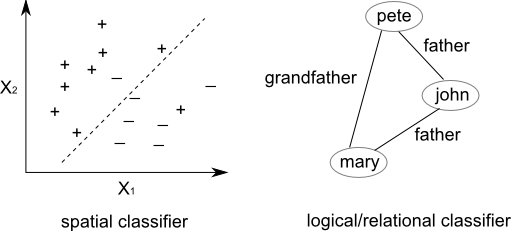
\includegraphics{spatial-vs-logical.png}
\caption{Spatial vs logical classification}
\end{figure}

To illustrate this with an example:  Let's think of how a child (AGI or human) learns the concept of (blood) relatives.  The child (Jane) would be given some examples of people around her and whether they are her relatives, eg:\\
\hspace*{1cm} father(jane, john), relative(john)\\
\hspace*{1cm} mother(jane, mary), relative(mary)\\
\hspace*{1cm} uncle(jane, pete), relative(pete)\\
\hspace*{1cm} neighbor(jane, joe), $\neg$relative(joe)\\
\hspace*{1cm} friend(jane, kate), $\neg$relative(kate)\\
and the task is to learn a general rule for relatives.  The solution can be stated quite succinctly\footnote{This solution is not entirely correct, as relatedness can grow unbounded and everyone would be ultimately blood-related.  Perhaps this problem can be resolved by fuzziness and other mechanisms such as non-monotonicity, but my point here is to show that the situation for propositional representation is even worse, as the problem appears insurmountable in that case.} in first-order logic:\\
\hspace*{1cm} relative(X, Y) $\leftarrow$ parent(X, Y)\\
\hspace*{1cm} relative(X, Y) $\leftarrow$ sibling(X, Y)\\
\hspace*{1cm} relative(X, Y) $\leftarrow$ married(X, Y)\\
\hspace*{1cm} relative(X, Y) $\leftarrow$ relative(X,Z), relative(Y,Z)\\
but it is very difficult to express in propositional logic unless we limit the domain of entities to a few people.  Also, we can see that \textit{spatial} statistical learning will fail to learn this rule because:\\
1. The dataset cannot be represented as numerical values in a vector space, or it could be done only very awkwardly.\\
2. Even when the dataset is cast in vector space, the learning algorithm can mostly learn to classify \textit{existing} examples, but the \textit{generalizations} would be wrong -- this is because the formulae in first order logic can entail discrete examples that are not necessarily located in a localized region in the numerical space.  Even if you carve the space into ridiculously complex regions, the next example would still be an exception because ``spatial compactness'' is simply absent in the underlying concept.\\
3. The child's world typically has very few people in it, yet she is able to learn the concept.  In ANNs and statistical learning, the sample size is typically at least 100s, but logic-based learning can learn the concept with just a few examples.

Although first-order representations can be converted to propositional ones via the process of propositionalization, such algorithms cost exponential time and space.  This is not difficult to see:  FOL allows us to express knowledge very succinctly.  There are some techniques that ameliorate the combinatorial explosion, such as partial instantiation (\citep*{Chandru1999}) or sparse matrix (\citep*{Domingos2008}).  But I still think it is easier and more intuitive to working on a FOL KB directly, especially for AGI.

And, despite propositionalization, the class of spatial statistical learning techniques still seem to be unsuitable for logic-based AGI because propositionalization does not cure the fundamental lack of ``compressiveness'' of predicate logic that I pointed out above.  (After propositionalization, some fast propositional SATisfiability algorithms can be invoked, but they are still qualitatively different from the spatial learning algorithms.)  From this consideration, my current strategy is to focus on algorithms specifically for FOL / HOL / predicate logic.

The application of kernel methods to logic seems to rely on syntactic distance rather than \textit{semantic} distance.  (Eg: \citep*{Muggleton2005} developed a support-vector ILP method;  \citep*{Gartner2008} describes a method that constructs kernels for (first-order and higher-order) logic formulae, based on a representation of logic by typed lambda calculus in \citep*{Lloyd2003}.  It involves the use of a ``matching kernel'' that measures syntactic distance only.)  So far I have not seen an effective way to estimate semantic distance without performing logical inference.

\{ Some new techniques have been developed to lift neural networks to first-order representations, but I have not examined them in detail (eg, \citep*{Garcez2009}, \citep*{Hammer2007}).  \}

\{ To-do:  I've gained some new insight into the issue of mapping predicate logic to continuous space, via algebraic logic. \}

\section{Why not neural network?}

There are several reasons why I think the NN approach may be less promising:

1.  First-order logic is a more powerful representation scheme than (feed-forward) neural networks (\S\ref{sec:why-logic}), whereas dynamic neural networks are very difficult to work with.

2.  A neuron is "fixed" within a network and cannot "move around", which seems to make it difficult to perform invariant pattern recognition (eg, translational, rotational, and scale- invariance in vision). The brain has to use neurons due to biological constraints, but it seems more effective to use other pattern matching methods on von Neumann machines. (Scale invariance is particularly difficult for ANNs, see \citep*{Muresan2004}.)

3.  Neural learning is slower and require a larger amount of examples. Logic-based learning is coarse-grained and thus require fewer examples to induce the correct representation, sometimes as few as 1 example.

4.  As Ben Goertzel pointed out some years ago, a network of redundant propositions can be reduced to a minimum number of non-redundant propositions, without loss of information;  the only thing that is lost is \textit{fault tolerance}.

However, neural networks may be used for handling low-level vision, especially at the feature-extraction level.

\section{Recursive self-improvement}
\label{sec:RSI}

RSI refers to the ability of an AGI to reprogram itself.  Some authors predict that the RSI point will trigger the Technological Singularity (eg \citep*{Kurzweil2005}).  I think the way to reach the RSI point with the least amount of efforts would be to build an automatic program synthesis tool that accepts natural-language commands or goal specifications.  From then on, we can use this tool to rewrite the tool itself and to evolve it (semi-automatically) into a full AGI system.

\section{Chicken-and-egg problem}
\label{sec:chicken-and-egg}

\begin{figure}[H]
\centering
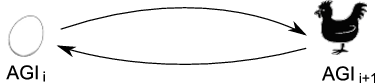
\includegraphics{chicken-and-egg1.png}
\caption{chicken and egg problem}
\end{figure}
\vspace{-0.5cm}

Anyone who has thought about AGI long enough will be aware of this problem:  The idea is to use a ``program evolver'' that takes an input program $\Pi_i$ and improves it to $\Pi_{i+1}$ according to some user-specifications.  We put the evolver through itself, thus building up its intelligence recursively without doing any programming (except for the initial evolver).

This idea (at least naively) does not work because the initial evolver needs to have very good background knowledge about programming or else it cannot perform its job in reasonable time.  \S\ref{sec:self-programming-architecture} discusses how to make it feasible.

\section{Natural reasoning}
\label{sec:natural-reasoning}

Other names for natural reasoning are: common-sense reasoning, human-like reasoning, informal reasoning.

Natural reasoning is an extension of logical reasoning with:\\
1.  ability to recognize natural concepts (which I posit requires fuzzy pattern recognition)\\
2.  ability to use metaphors, similes, analogies, and similarity-based reasoning

An example of natural reasoning is:

\leftskip 1cm \textit{Suppose I need to write a program to ``break English sentences into words''.  I'd need to declare a function to do this.  What would be the input and output of this function?}

\leftskip 0cm Note that in the above reasoning, I think of the function as a ``box'' with something that goes in and something out.

Natural reasoning is required to turn informal, natural-language statements into formal statements.  This is especially important to formal program synthesis.

\chapter{Architecture}
\index{architecture}
\minitoc

We will first look at various basic architectures and then try to decide on a final design.

\section{Logical reasoner (blackboard architecture)}
\label{sec:blackboard-architecture}
\index{architecture!blackboard}

This is an older design I explored around 2006, chiefly to put together several logic-based algorithms on a blackboard.  The following page is a schematic diagram showing various modules of the \textbf{logical sub-system}.

My intuition is that such a logical sub-system is essential to any AGI, but it should be built on top of a more basic, \textit{procedural} layer (cf \S\ref{sec:proc-subsumes-decl}, ``Procedural subsumes Declarative'').

\begin{figure}[H]
\centering
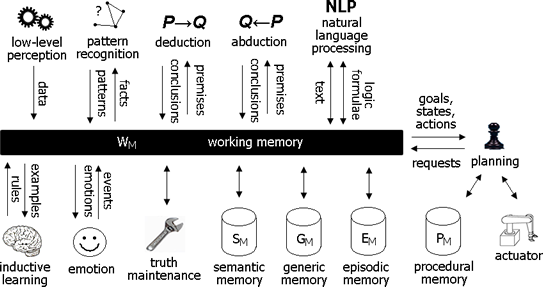
\includegraphics[width=5.65625in,height=2.9895833in,bb=0 0 543 287]{blackboard-architecture.png}
%\caption{AGI architecture}
\end{figure}

Here is a simple top-level algorithm to process incoming sensory events:

\begin{algorithm}[H]
\caption{Top-level sensory processing}
\alginout{raw sensory input}
{updated KB}
\begin{algtab}
\alglabel{alg:top-level-sensory-processing}

Upon the arrival of raw sensory input, perform \textbf{pattern recognition} (\S\ref{ch:pattern-recognition}) which is the same as forward-chaining (\S\ref{sec:deduction}).  (NL input can bypass this step.)  The result will be a set of \textit{new facts} and will be put in Working Memory.  Forward chaining can be performed several times on top of previous results.\\

Perform \textbf{consistency check} (\S\ref{sec:consistency-check}) on the new facts against the KB\\

If a new fact is inconsistent with the current KB, invoke \textbf{conflict resolution} (\S\ref{sec:conflict-resolution})\\

Perform \textbf{abduction} (\S\ref{sec:abduction}) on the new facts, so WM will make appropriate assumptions to account for them.\\

Invoke the \textbf{inductive learner} (\S\ref{sec:inductive-learner}), ie, try to compress the new facts + KB.\\
\end{algtab}
\end{algorithm}
\vspace{-0.6cm}

The abduction algorithm is almost identical to the consistency-check algorithm, so they may be merged.  The abduction algorithm is also very similar to the induction algorithm (cf \S\ref{sec:abduction}), so all 3 may be merged.

\section{BDI architecture}
\index{architecture!BDI architecture}

BDI (\textbf{belief-desire-intention}) is one of the most successful agent architectures ever proposed.  It was first investigated by Michael Bratman as a theory of human practical reasoning (\citep*{Bratman1987}), and later formulated as an agent architecture (\citep*{Bratman1988}).  The main concern of BDI is how to plan in the face of a \textit{dynamic environment} and with \textit{bounded resources}.

Key to BDI is the idea of \textbf{commitment}.  Once an agent commits to a plan, the plan will constrain means-end reasoning, thus making planning processes more efficient.

\textbf{B: Beliefs} are the contents of the KB.\\
\textbf{D: Desires} are unconstrained;  they need not be achievable or even consistent (eg, one can desire smoking and good health at the same time).\\
\textbf{I: Intentions} are goals that the agent commits to;  they are believed to be achievable and must be consistent.

\begin{figure}[t]
\centering
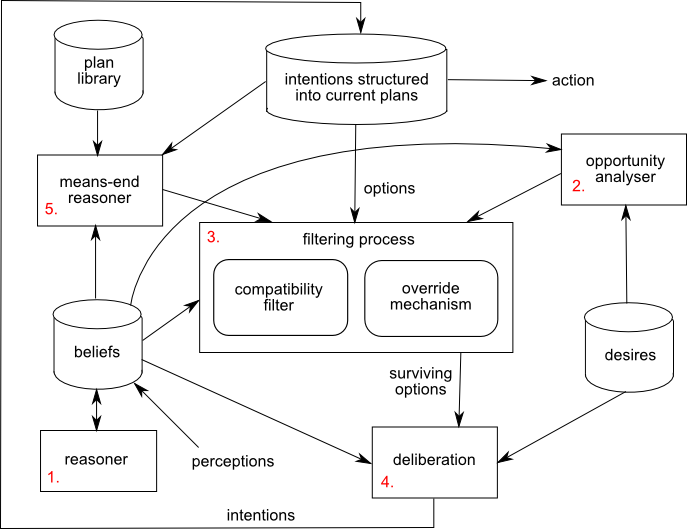
\includegraphics[scale=0.7]{BDI-architecture.png}
\caption{schematic diagram of the BDI architecture}
\label{fig:BDI-arch}
\end{figure}

Figure \ref{fig:BDI-arch} is a schematic diagram of BDI.  The key processing steps are:
\begin{compactenum-}
\item  This is the \textbf{Knowledge / Declarative Sub-system}, which we will consider at length in the rest of the book.
\item  Changes in the environment cause changes in beliefs, which in turn reveal new possibilities to satisfy desires.  Thus the \textbf{Opportunity Analyzer} tries to propose new \textbf{options}.
\item  Once the options are produced (either by the Opportunity Analyzer or the Means-end Reasoner), they are subject to \textbf{filtering}.  The \textbf{Compatibility Filter} checks if options are compatible with existing plans.
\item  Surviving options are weighted against each other by the \textbf{Deliberation Process}, which produces intentions to be incorporated as plans.
\item  The \textbf{Means-end Reasoner} searches for the next available options, taking into consideration the current plans.
\end{compactenum-}

\section{Evolutionary architecture}

\{ TO-DO:  Hayek is not the correct designation for this architecture \}

Hayek is an artificial economy proposed by Eric Baum (\citep*{Baum2004}) as an AGI architecture.  A slight variant of Hayek can be described as follows:
\index{architecture!Hayek architecture (economic model)}

\begin{compactenum-}
\item The AGI is composed of a large number of small programs.
\item \textbf{Cooperativity}.  The programs may call each other.
\item \textbf{Persistent memories}.  Individual programs can remember things across time slices.
\item A \textbf{meta-controller} runs these programs according to some schedule, allotting each program a time slice.
\item \textbf{Credit assignment}:  If the program answers a question correctly or performs a good action (judged by some external critic), the meta-controller will credit the programs that have contributed to the result.
\item Human programmers may contribute to this pool of programs.
\end{compactenum-}

A high-level programming language (such as Lisp) seems to be more suitable for this purpose.

Note that even very complex algorithms can be implemented in this architecture.  For example, a best-first search algorithm can remember its search state in an external memory store.  Then it just waits for its time-slice to resume searching.  Thus human programmers can seed the artificial economy with highly competent programs.

\section{Decision-theoretic architecture}
\index{architecture!decision-theoretic}

This is mathematically more elegant than the BDI architecture.

Some important elements that should be present in the architecture:
\begin{compactenum-}
\item  \textbf{percepts} are raw (unprocessed) sensory events
\item  \textbf{beliefs} are the contents of the KB
\item  \textbf{states} --- all possible \textit{perceived} states of the environment, including the current state.  States are special terms in the logic.
\item  \textbf{actions}
\item  \textbf{utility function} --- a function $U: \{state\} \rightarrow \mathbb{R}$.  Utilities may be defined implicitly, though.
\end{compactenum-}

This architecture may depend on a \textbf{logical sub-system} that:
\begin{compactenum-}
\item  recognizes environmental states (eg \textit{``the apple is on the table''}) from raw percepts (eg pixel values from a camera)
\item  recognizes possible actions (eg \textit{``I can put the apple on the plate''})
\end{compactenum-}

The goal is to maximize expected utility.  Planning becomes a discrete optimization problem in this setting.

Reinforcement learning \index{reinforcement learning} can be naturally included in this architecture.

\section{Self-programming architecture}
\label{sec:self-programming-architecture}
\index{architecture!self-programming}
\index{programming!self-programming}

Consider this variant of the chicken-and-egg problem (\S\ref{sec:chicken-and-egg}), where we distinguish between the \textbf{Synthesizer} and the AGI:
\begin{figure}[H]
\centering
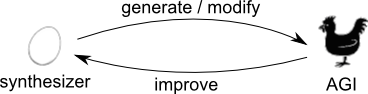
\includegraphics{self-programming-architecture.png}
%\caption{improved self-programming architecture}
\vspace{-0.5cm}
\end{figure}

Currently we know the following program-synthesis paradigms:\\
1.  human programming\\
2.  natural reasoning (NR), ie common-sense / human-like reasoning\\
3.  automated theorem proving (ATP)\\
4.  stochastic local search (SLS), including evolutionary algorithms (EA)\\
5.  reinforcement learning (RL) \index{reinforcement learning}\\
We will consider each paradigm in turn.

A key question is how an initially-dumb AGI can \textit{improve} the performance of the Synthesizer, even slightly.

\textbf{1. Human programming} (ie, brute-force software engineering without RSI)\\ \index{programming!human}
The problem with this approach is that it does not exploit the advantages of machine program synthesis, and thus is likely to be sub-optimal.

\textbf{2. Natural reasoning} (cf \S\ref{sec:natural-reasoning})
\begin{compactenum-}[(a)]
\item  The problem is that NR does not yet exist, but it is a \textit{sine-qua-non desideratum} of AGI.
\item  So the question is how to enable an initially weak form of NR to synthesize programs.  One possibility is to use \textbf{creativity}:  the AGI will generate programs by partly reasoning and partly random acting.
\item  An agent with NR is likely to have RL as well.
\item  An NR agent can invoke ATP.
\item  An NR agent can self-program (without invoking ATP), simply by \textbf{deductive planning} (\S\ref{sec:deductive-planning}).
\end{compactenum-}

\textbf{3. ATP} \index{programming!ATP (automated theorem proving)}
\begin{compactenum-}[(a)]
\item  It requires \textit{formal} specifications of programs (or sub-routines), which are often very hard to write for humans.
\item  Search in proof space can be very slow.
\item  There already exists ATP-based program synthesis software, which can be used externally.
\end{compactenum-}

\textbf{4. Stochastic local search} \index{search!stochastic local search}
\begin{compactenum-}[(a)]
\item  Is based on generate-and-test.
\item  ``Generate'' is random and the program space is typically huge.
\item  ``Test'' is often slow because it requires the entire AGI to answer a large number of benchmark queries.  A possible remedy is to specify input-out benchmarks for AGI \textit{components}, but then the burden is on humans to design the modular architecture.
\item  A large population of relatively low-score programs has to be maintained, in order to allow sufficient time for cooperativity to evolve.  For this reason I suspect that the evolutionary approach is rather slow.
\item  2 further problems are:  How can an initially-dumb AGI improve the stochastic searcher?\footnote{In MOSES (cite) an attempt is made at ``representation building''.} And how can this transfer of rationality from the AGI to the Synthesizer be coded once and for all?
\end{compactenum-}

\textbf{5. Reinforcement learning} \index{reinforcement learning}
\begin{compactenum-}[(a)]
\item  The goal of RL is to learn policies of how to act in certain environmental states.  It can synthesize programs if the environment is that of programming.
\item  RL can be augmented with logical reasoning.
\item  RL can implement the idea of expected utility maximization.
\end{compactenum-}

\textbf{Combining all methods}\\
Apparently, we can combine all the above methodologies without conflict:
\begin{figure}[H]
\centering
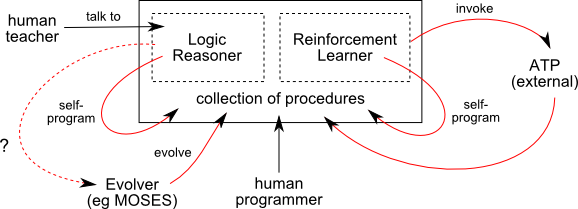
\includegraphics{combined-architecture.png}
\vspace{-0.5cm}
\end{figure}

The question is to choose the \textit{most effective} method of AGI self-programming (red lines).  My intuition is that the evolutionary method is much less efficient than the other 3 (it is easier to explain to children to do something than to train animals by reinforcement, which is in turn easier than breeding animals for the innate ability to do that thing), provided that some rudimentary ability of reasoning is present.

Maybe the most cost-effective method (from the human labor perspective) is to combine RL with logical reasoning and deductive planning --- for instance, to allow RL to invoke IE (inference engine) or vice versa.

\section{AIXI}

\underconst

\section{Distributive architecture}

This is a monolithic view of the inference engine.  For simplicity's sake, only the deduction part is shown, since deduction is the most essential core of the engine.

\begin{figure}[H]
\centering
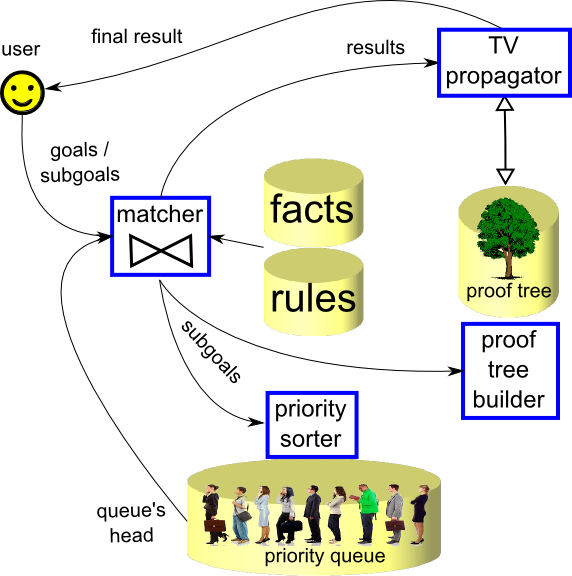
\includegraphics[scale=0.5]{breakdown-IE-1.png}
% \vspace{-0.5cm}
\end{figure}

This is a distributive architecture for deduction:

\begin{figure}[H]
\centering
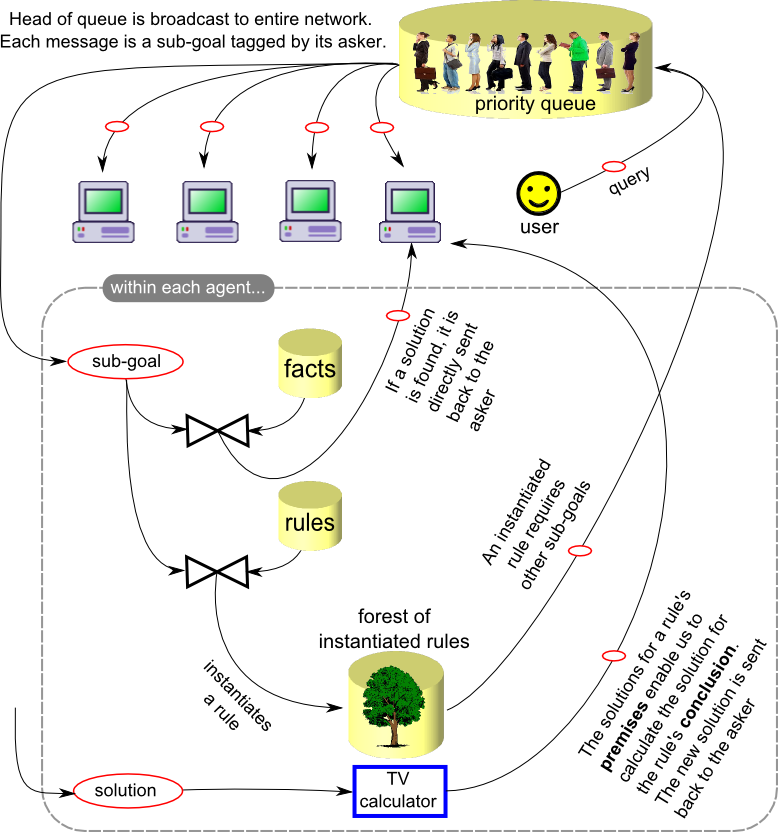
\includegraphics[scale=0.6]{breakdown-IE-2.png}
% \vspace{-0.5cm}
\end{figure}

Each agent responds to queries and spits out solutions. For example, an agent may have a rule in its (local) KB that "professors who wear sandals are nice to students".  The agent listens to queries, trying to find something it can answer.  A query such as "who is nice to students?" would be a hit.  Then the agent either:

\begin{compactenum-}
\item returns an answer, if it knows as a \textit{fact} that XYZ is nice to students.
\item applys a rule and returns one of more sub-goals;  In this case, the sub-goal is "does XYZ wear sandals?"  Wait for other agents to answer that.
\end{compactenum-}

In case \#2, if another agent provides an answer "Professor Matt Mahoney wears sandals", say with TV = 0.9, and sends it back to the first agent, then the first agent decides how to calculate the TV of the conclusion given that TV of premise = 0.9.  The only calculation it needs to perform is for the rule that it owns.  Then it returns the answer to the asker.

This architecture is so wonderful because there is no need to construct the proof tree anymore. The proof tree seems to have disappeared but it is really implicitly constructed among the network of agents and the messages!

Thanks to Matt Mahoney for proposing the CMR (competitive message routing) architecture.

\chapter{Knowledge representation}
\minitoc

\section{Introduction}

An AGI uses a KR structure to \textit{represent} the external world, and this structure is built with limited computational resources, and as such, must be approximate.  We have a lot of freedom to choose the KR format.

I chose logic as KR because it offers a \textit{direct} way to translate natural-language texts into machine knowledge.  This is of critical importance because the overall feasibility of AGI hinges on the efficiency of machine learning, and the most effective machine-learning method is ``learn by being told'' (\S\ref{sec:learn-by-being-told}).

A common misconception is:  ``How can complex ideas such as `John loves Mary' be reduced to logic formulae like \textit{loves(john,mary)}?''  One school of thought (see eg \citep*{Johnson-Laird1983}) posits that human reasoning is based on ``mental models'', but it is unclear how exactly they can be constructed.  My view of logic-based AI is that of using logic as a \textit{computational structure} for \textit{constructing} mental models.

% Sorted or unsorted logic?

\section{Multiplicity of knowledge representation schemes}

This is how I think of the issue of knowledge representation:\\
\begin{figure}[H]
\centering
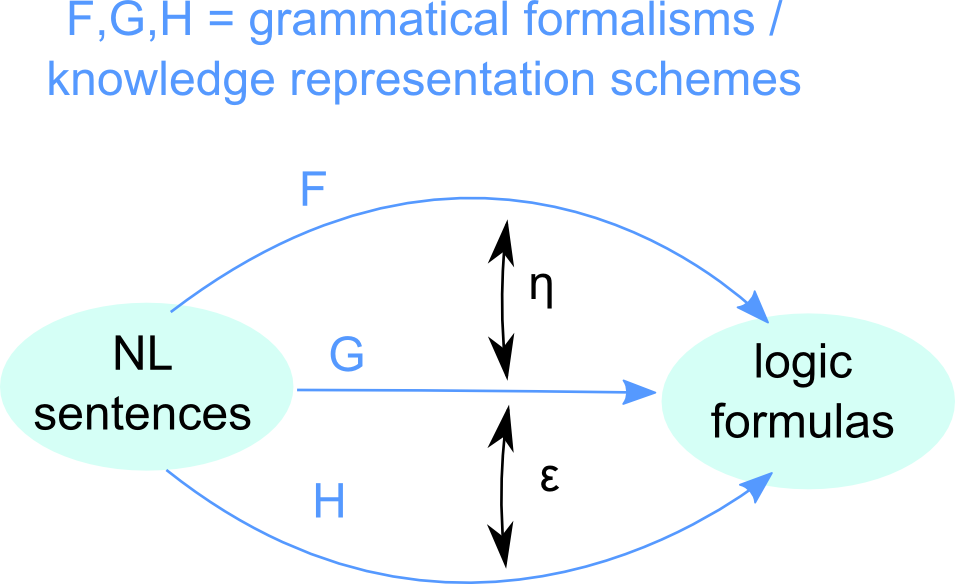
\includegraphics[scale=0.7]{KR-functors.png}
% \caption{KR functors}
\end{figure}

There are various KR schemes.  For example, in NL, there are various grammar formulations:\\
$F$ may be Phrase Structure Grammar\\
$G$ may be Fluid Construction Grammar\\
$H$ may be Categorial Grammar\\
$J$ may be Genifer's machine-learned grammar (which may be stochastic and inscrutable to humans)\\
$K$ may be some spatio-temporal KR scheme such as temporal logic, event calculus, situation calculus, etc

And then there would be transformations ($\eta, \epsilon, ...$) between the grammatical formalisms.

The problem is whether we can mix multiple KR schemes like $F$ and $G$.  The commonsense KB would be different under either $F$ or $G$, and the entire KB needs to be transformed by some $\eta$.

If we use $F, G, H,...$ at the same time, confusion may arise during machine learning and reasoning.

Perhaps, if we make Genifer be aware of transformations like $\eta, \epsilon, ...$ then maybe it can deal with multiple KR schemes at the same time?  Therefore we maybe don't need to choose or commit to any particular KR scheme at this stage...  in other words, any would be fine.

\section{Natural language}

Please also see the chapter on natural language (\ref{ch:natural-language}).

\subsection{Composition of concepts}
\label{sec:composition}

In 1928 the young Haskell Curry started working on \textbf{combinatory logic} (CL) as a \textit{logica universalis}, but it ran into inconsistency problems \footnote{In Genifer we try to use fuzzy-probabilistic truth values to get around this problem (see \S\ref{sec:paradox}).}.  One special feature of CL is \textbf{combinatorial completeness} -- meaning that any concept can, in principle, be applied to any other concept.  One can readily see that, when the concept of \textit{self-application} is applied to itself, it can lead to Russell's paradox (\S\ref{sec:paradox}).

Nevertheless, combinatorial completeness is something desirable in a universal logic.  It enables a logic to \textit{reason about logical paradoxes themselves}.  Bertrand Russell invented \textbf{type theory} to get around the problem of paradoxes, basically by banning all circular references.  But as a result of that, type theory (and thus the higher-order logic built on top of it) cannot be used to reason about paradoxes.

Curry's combinatory logic can represent arbitrary combinations of concepts, in a manner such as:\\
\tab $\lceil$wisdom$\rceil$ $\bullet$ $\lceil$socrates$\rceil$ = $\lceil$the wisdom of socrates$\rceil$

One of my latest insights is that the combination of concepts can be computed by the same process as \textbf{unification} of terms in logic.  For more details, refer to \S\ref{sec:unification}.

In 1963 JA Robinson discovered resolution, which is really unification + propositional refutation.  Unification decides if 2 terms can be made equationally identical.  Propositional refutation is an inference step that deals with the "calculus of thinking" at the \textit{sentence} level.

Around the 1900s, George Boole, CS Peirce, Gottlob Frege, amongst others, developed \textbf{predicate logic}, which is later popularized by people such Hilbert, Ackermann, Russell, and Whitehead.  Predacate logic has really been popular for only about 80 years, versus syllogistic logic that has been around since Aristotle's time.  Predicate logic differs from propositional logic by giving propositions \textit{internal structure} -- a proposition is broken down into a \textbf{predicate} and one or more \textbf{objects}.  However, this decomposition seems inadequate to deal with arbitrarily free combinations of concepts.

Combinatory logic provides a free way to compose terms via "application".  The key is to regard terms as (compound) concepts.  For example, in Genifer's notation:\\
\tab \english{tall handsome guy}\\
is the combination of the concepts\\
\tab (tall, handsome) $\circ$ guy.

Now, a few examples:\\
\english{tall handsome guy} is equivalent to \english{handsome tall guy};\\
\english{very tall guy} implies \english{tall guy};  but\\
\english{very tall guy} does not equal \english{tall very guy};

Thus the unification is modulo some special rules such as commutativity, associativity, etc, and certain reduction rules.  In other words, unification modulo a theory = "the calculus of concepts".

So we have a neat decomposition:\\
\tab calculus of thoughts = calculus of concepts + calculus of propositions

In \textbf{category theory}, one enforces the associative composition of arrows:\\
\tab $(ab)c = a(bc)$. \footnote{We often omit the application symbol $\circ$.}\\
Likewise, I observed that if we enforce the associative composition of concepts, the logical form becomes very elegant.  Due to associativity, any pair of concepts in an application:\\
\tab $a \circ b$\\
must be \textit{meaningful} in a meaningful sentence.

A consequence of enforcing associativity is that we can no longer use \textbf{Currying}.  For example:\\
\tab \english{John loves Mary}\\
would be rendered in Genifer's logic as\\
\tab \formula{((mary loves) john)}\\
rather than as suggested by Currying:\\
\tab \formula{((loves mary) john)}

Thus, in Genifer's logic, the 2 primitive operations are:\\
\tab 1. \textbf{application}, $\circ$\\
\tab 2. \textbf{pairing}, or cross product, $(a,b)$\\
with the associative and distributive rules:
$$ (a \circ b) \circ c = a \circ (b \circ c) $$
$$ (a, b) \circ c = (a \circ b, a \circ c)$$

One can recognize that this logic has the exactly form as a category.  \todo{I'm curious as to the role of exponentiation in this category?}

For more about how natural language sentences are translated into logical form, see the section on natural language and Geniform, \S\ref{sec:geniform}.

\subsubsection{Dynamic interpretation of semantics}

Look at these examples:\\
\tab \underline{glass slippers} are made of glass\\
\tab a \underline{door knob} is part of a door\\
\tab \underline{street prostitutes} work on the streets.\\
However,\\
\tab \underline{glass slippers} do not work in glasses\\
\tab a \underline{door knob} is not made of doors\\
\tab \underline{street prostitutes} are not part of the streets.

This suggests that the \textbf{semantics} of the compound concepts depend on \textit{external} pieces of knowledge, and hence must be interpreted \textit{dynamically}.  This is essentially the same idea as the abductive interpretation of natural language (\S\ref{sec:abduction-as-interpretation}).

\subsection{Reification}
\label{sec:reification}

Reification means ``to turn into objects''.  For example:\\
\tab \english{John loves Mary}\\
can be rendered as\\
\tab \formula{loves(john, mary)}\\
but\\
\tab \english{John loves Mary deeply}\\
would have to rendered as:\\
\tab \formula{love(love$_1$)} \tab \tab ; love$_1$ is an instance of love\\
\tab \formula{subject(love$_1$, john)}\\
\tab \formula{object(love$_1$, mary)}\\
\tab \formula{deep(love$_1$)}.

Notice that in the reified form, the original base-level formula:\\
\tab \formula{loves(john, mary)}\\
is lost!  This is rather unsatisfactory.

Geniform solves this problem by eliminating reification.

\section{Representing time}

As Einstein would have said, the representation scheme for space and time should be fundamentally the same.  As I have developed a vision theory (\S\ref{ch:vision}), I think temporal representations can follow a similar scheme.  OpenCog (http://www.opencog.org) is an AGI project more focused on embodiment, so we can also share their KR scheme.

\section{Contexts}

An excellent survey of contexts in logic-based AI is \citep*{Akman1996}.  The book \citep*{Sowa2000}, Chapter 5, is also excellent and contains additional insights about contexts.  Also the book \citep*{Bonzon2000}.

In Genifer, a context is just a set of propositions that are \textit{true in that context}.  This idea is very useful in the clustering of the KB for inference speed-up (\S\ref{sec:hi-oracle}).

\section{Assumptions and counterfactuals}

How to make assumptions during inference?  \english{Assuming mom is at home, I call her phone number.}

Example of a counterfactual conditional:  \english{If Oswald did not kill kennedy, someone else would have.}

\chapter{Slideshow: logic}
\chapter{Logic}
%\begin{flushright}
%\end{flushright}
\minitoc

Note:  This chapter is currently very chaotic because of a re-organization effort.  $\mathcal{Z}$ is no longer considered a foundational part of the logic.

\section{Background}

\subsection{Turing completeness}

\textbf{Undecidability of FOL.}

\subsection{$\lambda$ calculus}

(See Wikipedia: \href{http://en.wikipedia.org/wiki/Lambda_calculus}{Lambda calculus}).

\textbf{Bound variables:}  In the abstraction $(\lambda x.t)$ we call $x$ the bound variable and $t$ the body.  Every occurrence of $x$ in $t$ is \textbf{bound} by the abstraction.  Conversely, an occurrence of a variable $y$ is \textbf{free} if it is not bound, eg in $(\lambda z.(\lambda x.(yx)))$.

\textbf{Head-normal form:}  A $\lambda$ term is in head-normal form if, for $m \geq 0$ and $n \geq 0$, it can be expressed as:
$$\lambda x_1 ... x_m . x t_1 ... t_n$$.
The variable $x$ may either be free or bound (one of $x_1,...,x_m$).

\textbf{De Bruijn indexes.}

\textbf{Director strings.}

\subsection{Combinatory logic}

(See Wikipedia: \href{http://en.wikipedia.org/wiki/Combinatory_logic}{Combinatory logic}).

Bound variables -- why they are confusing?

\subsection{Term-rewriting systems}

\subsection{Simple type theory}

\subsection{Higher-order logic}

\textbf{Standard semantics and general semantics (of higher-order logic).}

Why Henkin semantics is a reduction to FOL?

\subsection{Model theory}

\subsection{Proof theory}

\subsection{Deduction systems}

\textbf{Hilbert systems.}

\textbf{Natural deduction.}

\textbf{Sequent calculus.}

\textbf{Tableau.}

\textbf{Resolution.}

\subsection{Paradoxes in logic}

\textbf{Liar's paradox.}

\textbf{Skolem's paradox.}

\textbf{Tarski's paradox.}

\textbf{Non-axiomatizability.}  ``First order logic has an effective notion of proof which is complete w.r.t. the intended interpretation.  This is the content of Godel's completeness theorem.  As a result, the set of (Godel numbers of) universally valid first-order formulas is recursively enumerable.''  But ``the set of second order validities is not arithmetically definable let alone recursively enumerable and hence that an effective and complete axiomatization of second-order validity is impossible'' \citep*{Benthem}.

\subsection{Functional programming}

\section{Logic and pre-logic}

Designing the perfect logic is nearly impossible, as witnessed by the proliferation of alternative logics in recent decades.  \textbf{Pre-logics}, or logical frameworks, are attempts to reduce logics to simpler computational mechanisms, and thus to tackle the problem in a general way.

The candidates for pre-logics include:
\begin{compactenum}[\textbullet ]
\item $\lambda$ calculus
\item combinatory logic
\item term-rewriting systems
\item grammars
\item programs (such as genetic programs)
\item etc
\end{compactenum}

The basic configuration of a system with pre-logic is like this:
\begin{figure}[H]
\centering
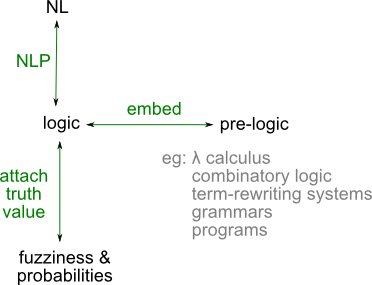
\includegraphics[scale=0.7]{prelogic.png}
% \caption{Prelogic}
\end{figure}
NL should be translated into logic because logic is closer to NL than pre-logic.  What really distinguishes ``logic'' from pre-logic is the notion of \textbf{propositions}, which is a unit of meaning to which we can attach \textbf{truth values}.  A proposition such as \formula{male(john)} is a ``complete'' entity of meaning, as opposed to the predicate \formula{male} which is incomplete, or ``syncategorematic''\footnote{The term syncategorematic has several meanings, here I mean any component of a sentence that is not a proposition.}.  This distinction is important because fuzziness and probabilities should be assigned to the logic rather than pre-logic.

The problem with the above configuration is, if the pre-logic is fixed and the logic is allowed to be dynamically learned, then it may be difficult to work with such a dynamically changing logic, in particular to assign fuzzy-probabilistic truth values to it, or to translate NL to it.

\section{Uncertainty}

Reasoning under uncertainty is a vast and nightmarishly complex topic in AI.  Simon Parsons's book \citep*{Parsons2001} contains a very good survey of uncertain reasoning, but even that is not exhaustive.  We may look at the following taxonomy of ``ignorance'' proposed by \citep*{Bosc1997}:
\begin{figure}[H]
\centering
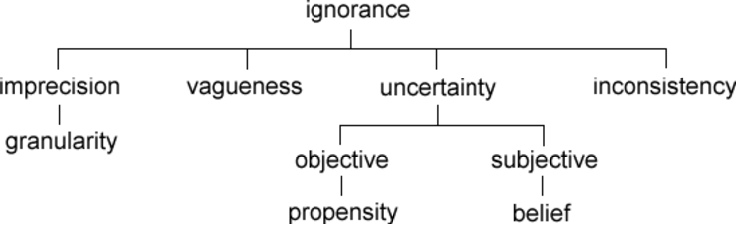
\includegraphics[scale=0.7]{IgnoranceTaxonomy.png}
\caption{taxonomy of ignorance}
\end{figure}

At first blush, classical logic appears to be sufficient for AGI.  Some AGI designers prefer to use crisp logic as the base and plan to build $\mathcal{P}$ and $\mathcal{Z}$ upon crisp logic.  But this may be a sign of not facing problems and not having sufficient understanding of fuzzy-probabilistic logics.  To represent $\mathcal{P}$ and $\mathcal{Z}$ logic \textit{in} crisp logic is like writing an entire $\mathcal{P}$-$\mathcal{Z}$ inference engine in Prolog, complicated by the fact that the crisp logic would be somewhat different from Prolog and so may be even harder to program in.  Also, the ``truths'' known by the AGI will then be different from the truths as represented in the crisp logic --- the former would be ``floating'' above the latter;  This creates unnecessary indirectness.  I will give other reasons in \S\ref{sec:whyZ} and \ref{sec:whyP}.

\textbf{Why not include other uncertainty measures besides $\mathcal{P}$ and $\mathcal{Z}$?}

There are other theories of uncertainty, such as possibility, belief functions, and rough sets.  The reason I chose $\mathcal{P}$ and $\mathcal{Z}$ is because they are simple and best understood.  There has been attempts to create systems where the user can create a flexible number of uncertainty measures, but one problem of such systems has been pointed out in \citep*{Parsons2001}:  If we have 3 uncertainty measures, say ``cloud'', ``mist'', and ``fog'', there would be a need to provide mixed inference rules for ``cloud-mist'', ``cloud-fog'' etc, a total of $n^2$ possibilities.  I have worked out the combination of $\mathcal{B}$, $\mathcal{P}$ and $\mathcal{Z}$ and found that it involved considerable efforts.

\section{Nonmonotonicity and defeasible reasoning}
\label{sec:exceptions}

One can create defeasible logics from classical logic, for example Reiter's \textbf{default logic} and McCarthy's \textbf{circumscription}.  But the classical approaches seem to require enumerating all possible exceptions, which is impractical.

\textbf{2 examples:}

\textbf{A.}\\
\textit{
1. John is usually very punctual.\\
2. Therefore, John will arrive at the airport on time.\\
3. John has an accident en route to the airport, and dies.\\
4. Therefore, John will NOT arrive on time.\\}
Will John arrive on time?

\textbf{B.}\\
\textit{
1. Mary has cybersex with many partners.\\
2. Cybersex is a kind of sex.\\
3. Therefore, Mary has many sex partners.\\
4. A person who has many sex partners has a high chance of STDs.\\
5. Therefore, Mary has a high chance of STDs.}

What's wrong with example B?  On the one hand, we should admit that cybersex is sex (it is a borderline case), but it lacks certain prominent features of sex, such as physical contact (which is not necessarily a \textit{defining} feature of sex).  Thus, if we carry on reasoning with the idea that cybersex is sex, we may get unsound conclusions.  The key to resolving this problem is to recognize ``cybersex is sex'' with \textbf{qualifications} such as ``it is sex without physical contact''.

If we have a rule that ``sex transmits certain diseases'', we may have to attach the exception ``only if the sex involves physical contact''.  In the end, our rules may be inundated with possibly infinitely many exceptions.  How can we get out of this problem?

\citep*{Wang1994}, \citep*{Wang2006} in NARS provided a solution.  His idea is not to store the exceptions to rules, but instead allow a \textit{multitude} of rules to fire, calculate the ``confidence'' (\S\ref{sec:confidence}) of each conclusion, and pick the conclusion with the highest confidence.  This allows us to handle exceptions relatively easily.

For the example:
\begin{eqnarray}
X \PimpL A \nonumber \\
X \PimpL B \nonumber
\end{eqnarray}
Pei Wang's idea is to calculate the combined conditional probability by weighing each individual conditional probability with their associated \textbf{confidences} (\S\ref{sec:confidence}):
$$ P(X|A,B) = \frac{ P(X|A)c_A + P(X|B)c_B }{ c_A + c_B } $$
which is a nice idea\footnote{Except that NARS truth values do not conform to probability theory.}, but Abram Demski came up with an alternative idea that is more in accord with Bayesianism.  The idea is to reconstruct $P(X|A,B)$ from the marginal conditionals $P(X|A)$ and $P(X|B)$ and priors $P(A)$ and $P(B)$.  This is achieved by applying Bayes' rule twice:
\begin{eqnarray}
P(X|A,B) &=& \frac{P(A,B|X)P(X)}{normalization} \nonumber \\
         &=& \frac{P(A|X)P(B|X)P(X)}{normalization} \nonumber \\
         &=& \frac{P(X|A)P(A)P(X|B)P(B)}{P(X) \; normalization}
\end{eqnarray}

\{ To-do:  Abram's solution seems problematic, I'm discussing it with him... \}

\section{Equality}
\index{equality}  \index{identity|see{equality}}
\label{sec:equality}

A problem with equality is illustrated by the classic example ``Morning Star / Evening Star''.  This is a similar example and its rendition in logic:\\
\tab
\begin{tabular}{l|l}
\textit{``Clark Kent is Superman.''}               & \formula{clark-kent = superman} \\
\textit{``Superman can fly.''}                     & \formula{can-fly(superman)} \\
\textit{``Mary does not know that Clark Kent is Superman.''} & $\neg$ \formula{know(mary, "clark-kent = superman")} \\
\textit{``Mary knows that Superman can fly.''}     & \formula{know(mary, can-fly(superman))} \\
\textit{``Mary does not know that Clark Kent can fly.''} & $\neg$ \formula{know(mary, "can-fly(clark-kent)")}
\end{tabular}

Perhaps the solution is that \formula{"clark-kent"} (in quotes, ie, the Clark Kent that Mary knows) is not equal to \formula{clark-kent} (without quotes, ie, the real Clark Kent).

\section{Modal logic}
\begin{flushright}
\emph{Modality, si! Modal logic, no!}\\
--- John McCarthy
\end{flushright}

My view is to use predicates to represent modality instead of using modal logics.  This view was first advocated by \citep*{McCarthy1997}.

One argument for the use of modal logic arises from the previous example:\\
\begin{tabular}{l|l}
\hspace*{1cm} \textit{``Mary believes Superman is dead.''} & \formula{believe(mary, dead(superman))}\\
\hspace*{1cm} \textit{``Superman is Clark Kent.''} & \formula{superman = clark-ken}\\
\hspace*{0.7cm} * \textit{``Mary believes Clark Kent is dead.''} & \formula{believe(mary, dead(clark-ken))}
\end{tabular}\\
but Mary may not know that Superman is Clark Kent.  This problem can be resolved as in the last section (\S\ref{sec:equality}).

\section{Shortcomings of the current logic}

1.  \textbf{Binary vs $\mathcal{P/Z}$.}  It may be desirable to have binary logic alongside $\mathcal{P/Z}$ logic.  $\mathcal{P/Z}$ reasoning is suitable for common-sense concepts, whereas binary reasoning is good for \textit{programmatic}
\footnote{Ie, binary logic makes programming easier}
or computational reasons.  However, one unsolved problem is that many common-sense concepts appear to be binary but are fuzzy upon close inspection (eg male/female, dead/alive).  The question is how to let binary and fuzzy concepts coexist in the same logic.

2.  \textbf{First-order vs Higher-order logic.}  Let us admit outright that FOL as a KR scheme is insufficient for common-sense reasoning and thus AGI.  But I also have the impression that second-order logic would be sufficient for most common-sense reasoning purposes.

With some tricks (such as reification, \S\ref{sec:reification}), FOL may be able to deal with second-order reasoning.

Another trick is that the FOL reasoner can ``escape'' to a meta-reasoner when higher-order constructs are needed.  This will be taken up on the chapter on meta-reasoning, \S\ref{ch:meta-reasoning}.

As a more satisfactory long-term solution, we are currently working on creating a $\mathcal{P(Z)C}$ HOL, see \S\ref{sec:HOL}.

%With P and Z, the AGI can express ideas such as:\\
%\hspace*{1cm} ``Mary is \underline{probably} \underline{fairly} tall.''

\section{$\mathcal{B}$: binary logic}
\label{sec:binary-logic}

My intuition is that common-sense reasoning involves mainly $\mathcal{B}$, followed by $\mathcal{Z}$, and $\mathcal{P}$ is relatively rare.

%Horn clauses:  P and Z rules can be expressed in Horn form only.  But it seems that we can use general resolution for B rules, no?  Or, perhaps I want to use something similar to Horn resolution for P and Z?

%Each rule will enable one inference step, so the logic is almost truth-functional.  The problem is the intermediate results... I only know how to do that in B form.  Maybe we can keep a set of disjunctions of truth values?

%In B logic the proof procedure keeps a current clause / or a line of clauses.  In Bayes net we have a query variable and the algorithm finds its P value.  Z logic may be similar to B logic because it's truth functional?

%Perhaps we can work out the general case of a query variable of any TV type?  If we draw a B rule that's easy.  If Z rule, then we have a few Z variables as goals.  They need Z rules to fulfill, but what if we have a B rule for one of the sub-goals?  Then we need to translate the B value to Z value.  We can only do that via P(Z).  So we have a P(Z) value as one of the subgoals.  This may cause the head of the rule to become P(Z) too.  It seems there is a tendency for all TVs to become P(Z).
%That will actually back-propagate along the proof sequence.

%Things may be even worse for a P rule.  The application of the rule requires other numbers.  

\section{Meta-reasoning}
\begin{flushright}
\emph{I think I think, therefore I think I am.}
\end{flushright}

The term ``meta-reasoning'' may refer to 2 things:\\
1. The ability to \textbf{reason about reasoning}, which is what this chapter is concerned with;\\
2. Scheduling reasoning tasks to achieve best results with limited computational resources (I have not thought about this problem yet).

An excellent survey of meta-reasoning in the \#1 sense is \citep*{Constantini2002}.

In the Tell-Learn loop, we see that we need a special predicate credible() to increase the probability of a statement via a side-effect.  But that may not be the only meta-reasoning move we can make.

Another example is the $B \leftrightarrow Z$ conversion of ``traitor'' and ``patriot'' (\S\ref{sec:PZ-meta-reasoning}).

\section{Higher order logic}
\label{sec:HOL}

The HOL formulation that I am most familiar with is \citep*{Lloyd2003}.  It uses \textbf{typed lambda calculus} to represent logical formulae.  This representation is specifically developed for use as a logic programming language (Escher) and for inductive learning.

Interestingly, Lloyd uses a form of algebraic logic that is similar to what I do with $\mathcal{P(Z)C}$ logic, ie, its statements are of the form $H = B$ where $H$ is the head and $B$ is the body.  In essence this is the Prolog / Horn tradition.

\{ TO-DO:  formulate a $\mathcal{P(Z)C}$ HOL \}

\label{sec:PZ-meta-reasoning}

One example of meta-reasoning pertinent to fuzziness is:\\
\hspace*{1cm} S1: ``You are either a patriot or a traitor.''\\
\hspace*{1cm} S2: ``No, I can be slightly patriotic or slightly traitorous.''

In S1 the predicates \textit{patriot} and \textit{traitor} have binary character.  In S2 they have fuzzy character.

\underconst

\chapter{Vagueness ($\catZ$)}
\label{ch:vagueness}
\begin{flushright}
\emph{An approximate answer to the right question is better than\\
a precise answer to the wrong question.} --- John Tukey (rephrased)
\end{flushright}
\minitoc

NOTE:  this section will be re-formulated soon.  In the new version I only make 2 assumptions:

1. There are some quantities known as "degrees" and they are normalized to [0,1].

2. There exist relations amongst these quantities captured by \textbf{statistical models}.

I think the new formulation will be fairly unblemishable and uncontroversial, as opposed to earlier forms of fuzzy logic which many people are skeptical of.  But the new version also falls out of the classification as logic and is more of a fuzzy-probabilistic calculus.
\\

\footnotesize
I use $\catZ$ instead of $\mathcal{F}$ to denote fuzziness partly in recognition of Lotfi Zadeh's contributions, and also because $F$ and $f$ are often used for the CDF and PDF in probability theory, which may cause confusion when probabilities and fuzziness are used together.

A note on the examples used in this book:  some of them are politically incorrect or somewhat embarrassing.  I prefer examples that are simple, realistic, and relevant to human emotions because they help us think more clearly (cf the Wason selection task).  Usually I just choose the most obvious examples that come to mind.
\normalsize

\section{Vague phenomena}

There seems to be 3 types of concepts (= predicates).

The first type is \textbf{discrete} in nature, for example\footnote{I will later argue that even these concepts are not completely binary.}:\\
\hspace*{1cm} sex of a person $\in$ \{ male, female, hermaphrodite, trans-sexual \}\\
\hspace*{1cm} marital status $\in$ \{ single, engaged, married, divorced \}

The second type represents \textbf{numerical} measures, for example:\\
\hspace*{1cm} height \hspace*{1cm} weight \hspace*{1cm} age

The third type is not strictly numerical, but is often associated with ``\textbf{gradedness}'':\\
\hspace*{0.8cm} \begin{tabular}{l l}
beautiful    & ugly\\
intelligent  & dumb\\
simple       & complex\\
interesting  & boring\\
good         & bad\\
easy         & difficult\\
friendly     & hostile\\
clear        & unclear
\end{tabular}

There is no doubt that these predicates can be modified with degrees like ``very'' or ``slightly''.  But we do not know of any exact measures of their degrees.  For example, IQ has been proposed as an inexact measure of intelligence.  Most people would agree that there is some general consensus as to what is intelligent.  Such concepts exhibit \textit{vague phenomena}, which are characterized by:\\
\hspace*{1cm} 1. borderline cases\\
\hspace*{1cm} 2. lack of sharp boundaries\\
\hspace*{1cm} 3. susceptible to sorites paradox\footnote{A solution to the sorites paradox is given in \citep*{Bergmann2008} p268-282, using fuzzy logic and the notion of \textit{decaying validity}.}\\
\hspace*{1cm} 4. open-texture (ie, if $x$ is a borderline case, one can assert either $Q(x)$ or $\neg Q(x)$ in different contexts)

In philosophical logic, there are a number of theories of vagueness (see eg, \citep*{Graff2002}, \citep*{Keefe2000}, \citep*{Shapiro2006}).  $\catZ$ logic is a kind of Degree Theory (\citep*{Edgington1992}, \citep*{Sainsbury1986}), that uses numerical truth values to represent vagueness.  There are other non-numerical theories such as Epistemicism (\citep*{Campbell1974}, \citep*{Williamson1994}), and Supervaluation (\citep*{Fine1975}, \citep*{Keefe2000}).

\section{Why vagueness is needed for AGI}
\label{sec:whyZ}

One of the critical capabilities of AGI is (self-)programming.  Also, it is imperative to be able to instruct an AGI to write programs according to \textit{natural language} specifications and with robust common-sense background knowledge.  common-sense reasoning and natural language understanding depend on the use of vague concepts.\footnote{Vague concepts are not required for formal reasoning tasks such as formal mathematics and programming according to formal specifications.}  Look at any (technical or non-technical) natural-language text, and one finds that (explicit or implicit) vague concepts are ubiquitous.  It seems to be occur even more frequently than the (explicit or implicit) use of probabilities.

\textbf{Ubiquity of vagueness in common-sense reasoning.}  Some examples are:\\
\textbullet \, Time: \textit{Mother died \underline{a few days ago}}\\
\textbullet \, Space: \textit{One bird flew \underline{over the cuckoo's nest}} \hspace*{0.5cm} (lacking exact boundaries)\\
\textbullet \, Physics of liquids: \textit{A liquid in bulk and at rest has a horizontal surface}\\ (Is soup a liquid? ``In bulk'' is a fuzzy concept. Is the sea at rest? Surface tension can cause surface to curve)\\
\textbullet \, Physics of solids: \textit{A solid object cannot go from inside to outside a closed box}\\  (``Solid object'' is a fuzzy concept (eg a block of ice, a cat, a bomb). A card box may have small holes. The lid may be slightly ajar.)
%\textbullet \, Minds: 
%\textbullet 
%\textbullet 

\section{Why \textit{numerical} vagueness?}

The controversy is whether vagueness should be managed \textbf{quantitatively} (such as $\catZ$) or \textbf{qualitatively}.

One objection is that fuzzy logic can sometimes lead to unsound conclusions.  This problem is discussed in \S\ref{sec:exceptions} on nonmonotonic reasoning.

Having numerical vagueness allows us to:\\
1. Represent quantitative rules.  For example:\\
\hspace*{1cm} \begin{tabular}{l l l}
smart & $\leftarrow$ eloquent    & (the more articulate the smarter)\\
      & $\leftarrow$ humorous    & (the more humorous the smarter)\\
      & $\leftarrow$ insightful  & (the more insightful the smarter)\\
      & $\leftarrow$ creative    & (the more creative the smarter)\\
      & $\leftarrow$ etc...      &
\end{tabular}\\
2. Add up graded factors.  For example:\\
\hspace*{1cm} ``John is eloquent, humorous, insightful and creative'' $\rightarrow$ 0.9 smart\\
\hspace*{1cm} ``John is humorous and nothing else'' $\rightarrow$ 0.6 smart\\
3. Accrue contributing factors of a concept over a long period of time:\\
\hspace*{1cm} ``From my long experience with John, he is 0.9 smart''.

On the other hand, if we do not use numerical vagueness, we face these problems:\\
1. Failure to recognize ``partial'' concepts.  For example:\\
\hspace*{1cm} ``John is 0.7 smart'', or\\
\hspace*{1cm} ``tomato is 0.7 a fruit''\\
2. Conversely, failure to ignore ``very weak'' partial concepts.\\
3. Each statement must be attached with many qualifications, and they keep accumulating. Each rule would have to recognize a large ``exception set''.

The solution I adopt is to use both qualitative and quantitative information, by representing facts \textit{redundantly} (\S\ref{sec:exceptions}).  For example:\\
\hspace*{1cm} ``John is smart'', $z = 0.7$ (quantitative)\\
\hspace*{1cm} ``But he is only penny wise'' (qualitative)

Lastly, what if we don't need the precision of numerical vagueness in some situations?  For example:\\
\hspace*{1cm} ``Is John really that smart?'' ``Not quite.'' (we don't know the exact degree of smartness)\\
or\\
\hspace*{1cm} ``John is slightly smarter than Peter.'' (but we don't know the exact difference)\\
In my theory, these cases can be handled by combining $\catP$ and $\catZ$.

%One suggestion is that we can always use \textit{qualitative} binary statements in place of quantitative ones:\\
%\hspace*{1cm} ``John is fairly intelligent''\\
%\hspace*{1cm} \texttt{intelligent$_1$(john), fairly(intelligent$_1$)}\\
%\hspace*{1cm} ``John is intelligent but only in small matters''\\
%\hspace*{1cm} \texttt{intelligent$_1$(john), qualifies(intelligent$_1$, "only in small matters")}\\
%For the second example, we may say that a person who is intelligent only in small matters is not very intelligent, and thus assign, \textit{eg} Z = 0.6, but some qualitative information would be lost using this numerical representation.

%\begin{tabbing}The following example suggests that at least some \textbf{ordinal} relations may be necessary:\\
%\hspace*{1cm} (A) recently there's been a lot of thefts\hspace*{2cm} \=`that's bad'\\
%\hspace*{1cm} (B) recently there's been a lot of rapes \>`that's very bad'\\
%\hspace*{1cm} (C) recently there's been a lot of murders \>`that's extremely bad' ''
%\end{tabbing}
%which seems to suggest that the severity of crimes has this order:\\
%\hspace*{1cm} theft $<$ rape $<$ murder\\
%but this general ordering can have exceptions depending on circumstances.

%This example shows that sometimes \textbf{quantitative} representations may be necessary:\\
%\hspace*{1cm} ``During the financial crisis,\\
%\hspace*{1cm} (A) many people committed suicide;\\
%\hspace*{1cm} (B) children were sold as prostitutes;\\
%\hspace*{1cm} (C) decades of savings were destroyed''
%So one may react with the feeling ``that's very bad''.  But how was ``\underline{very} bad'' inferred?  Assuming we have a KB that let us infer that:\\
%\hspace*{1cm} A $\rightarrow$ bad\\
%\hspace*{1cm} B $\rightarrow$ bad\\
%\hspace*{1cm} C $\rightarrow$ bad\\
%how can we deduce ``very bad''?  We have 3 heterogeneous contributing factors.  One plausible solution is to assign degrees of badness to each of A, B, and C, and then add them up.

%Note that this example should be a simple reasoning task involving only a few inference steps.

%If the 3 contributing factors \textit{add up} to yield ``very bad'' (even approximately), the individual factors must be \textit{numerical}.  Or, maybe it is a simple counting of contributing factors?  3 bad things?  Not very satisfactory --- the things can have varying degrees.

%``I'm even more sure I don't want to be prostitute, after seeing the bad conditions''.  This is binary.

%But sometimes a rule for a predicate has many antecedents and only some of them are satisfied.  In the binary approach we may qualify them as exceptions.  But there are often many factors that may contribute to a predicate such as $smart$ or $charismatic$.  If you have known John for 10 years there may have been many incidences where he was smart/dumb or charismatic/dull.  In that case we may want to ``add up'' all those contributions.  In other words, it may be desirable to use a single number to summarize a large number of contributions, as long as the contributions are not exceptional.

%Suppose the AGI wants to erect these hypotheses:\\
%\hspace*{1cm} kind $\leftarrow$ attractive\\
%\hspace*{1cm} humorous $\leftarrow$ charismatic

%What if Z is not needed.  All we need is to convert results to binary, qualified form?

%Also, might it be necessary to use numerical Z even for single inference steps?\\
%For example:\\
%sluttish $\rightarrow$ not good wife (Z to Z)\\
%criminal $\rightarrow$ should be punished (Z to Z)\\
%obscene $\rightarrow$ should avoid speaking (Z to Z)\\
%attractive $\rightarrow$ I like (Z to Z)

%During pattern recognition it is often necessary to recognize an entity \textit{partially}, for example, the picture below may be a ``0.7 face''.  It seems that fuzziness is needed at a very fundamental level.
%\begin{figure}[H]
%\centering
%\input{CrossEyesFace}
%\caption{a fuzzy face}
%\end{figure}

\section{Semantics of Z}

There is some confusion about the interpretation of fuzziness, which I will try to clarify here.  I am influenced by Pei Wang's ideas \citep*{Wang2006}.

$\catZ$ is a measure of \textit{degree} or \textit{gradedness}.  Standard fuzzy theory employs the ``membership function'' to represent \textit{the degree to which an element belongs to a class}, but there is no consensus as to how the membership functions are defined.  Let's think of ``the degree to which a person is smart'', is it really arbitrary?

While there are no exact procedures to measure vague concepts (eg smartness), it is mandatory that a common-sense machine should possess some ways of assessing them, just like the human brain does.  In my AGI this is achieved by having a comprehensive knowledgebase of rules (acquired via machine learning) that compute numerical degrees of concepts.  Such rules are mini-algorithms (or ``\textbf{micro-theories}''\footnote{The term is used informally, not referring to Guha's notion of micro-theories in Cyc.}) that are \textbf{emergent properties} of intelligent learning systems.  They establish a \textit{distributed and approximate consensus} of how to measure vague concepts.

From another perspective:  PCA (principal component analysis) can calculate the component of a dataset that represents its greatest variance.  For example, PCA may identify the male-female axis of a set of movie-goers, or the liberal-conservative axis of a group of politicians.  When we map this axis to [0,1], we can get a fuzzy value of the concept male/female or liberal/conservative.  This may answer the question ``where do fuzzy numbers come from?'' \footnote{Abram Demski suggested this to me in discussion.}

If we regard $\catZ$ as a measure of degrees, $\catZ$ theory is mathematically as rigorous as probability theory.  $\catZ$ is a measure of degrees just as the height $H$ is a measure of how tall an object is.  Also, the $\catZ$-value can be inexact just as $H$ can be inexact, but this inexactitude is modeled separately by \textit{distributing probabilities over $\catZ$} (\S\ref{sec:combinePZ}).

$\catZ$ is not an approximation of probability; \S\ref{sec:probabilistic-interpretation} gives a probabilistic interpretation of vagueness, but in practice we can treat $\mathcal{P}$ and $\catZ$ as \textbf{orthogonal} to each other.  Possibility theory defines fuzziness as a weaker form of probability (as non-additive probability), but this is not the approach of $\catZ$ logic.

Finally I want to dispel the myth that probability is mathematically more rigorously defined than fuzziness:

\begin{tabular}{|p{7.5cm}|p{7.5cm}|} \hline
probability is defined by Kolmogorov's axioms &
fuzziness can be defined by similar axioms (\S\ref{sec:fuzziness-axioms})\\
\hline
probability follows a rigorous calculus &
fuzziness follows a rigorous calculus\\
\hline
probability is a subjective measure that exists only in the mind &
fuzziness is a subjective measure\\
\hline
probability can be exactly calculated for some cases, eg: dice or coin &
fuzziness can be exactly calculated for some cases, eg: age, temperature\\
\hline
some probabilities in our mind have obscure origin, eg: predicting the outcome of an election &
some fuzzy values in our mind have obscure origin, eg: which leader is more charismatic\\
\hline
\end{tabular}

Quantum mechanics or Heisenberg uncertainty does not prove that probabilities exist in the physical world.  On the other hand, studies in chaos and complex systems reveal that macroscopic descriptions are emergent and distinct from microscopic descriptions even though the former can be reduced to the latter.  Thus the recognition of fuzzy macroscopic patterns is every bit as real as the subjective use of probabilities to describe physical systems.  Vague concepts are also useful in thinking about pure mathematics -- for example, recognition of fuzzy similarities may assist mathematical reasoning.

%Inference in $\catZ$ is also different from traditional fuzzy logic because it does not use the implication operator $\rightarrow$ (\S\ref{sec:Z-conditionals}).

\section{Probabilistic interpretation of vagueness?}
\label{sec:probabilistic-interpretation}

One way to interpret vagueness as probability is to interpret\\
\hspace*{1cm} $Q(x); \; z = z_0$\\
as\\
\hspace*{1cm} ``Among all possible contexts, $Q(x)$ is true with probability $z_0$''.\\
For example, if $smart(john); \; z=0.8$ then John is smart in $80\%$ of circumstances.

More examples:\\
\hspace*{1cm} \begin{tabular}{|l|l|} \hline
\textbf{z = 0.8}             & \textbf{Interpretation}\\ \hline
John is very smart           & John is smart in $80\%$ of circumstances\\ \hline
Peter is very fat            & Peter is fatter in $80\%$ of comparisons (with other folks)\\ \hline
Jane is very pretty          & Jane is judged pretty by $80\%$ of beholders\\ \hline
\end{tabular}

%Despite this interpretation, it is easier and more elegant to regard $\mathcal{P}$ and $\catZ$ as orthogonal to each other.  For example, if we have a rule that says ``the fatter a person, the clumsier s/he is'', we can represent it with this Bayesian network:
%\begin{figure}[H]
%\centering
%%LaTeX with PSTricks extensions
%%Creator: 0.46
%%Please note this file requires PSTricks extensions
\psset{xunit=.5pt,yunit=.5pt,runit=.5pt}
\begin{pspicture}(188.79882812,70.51660156)
{
\newrgbcolor{curcolor}{1 1 1}
\pscustom[linestyle=none,fillstyle=solid,fillcolor=curcolor]
{
\newpath
\moveto(43.5,20.99999895)
\curveto(43.5,9.68399895)(33.868,0.49999895)(22,0.49999895)
\curveto(10.132,0.49999895)(0.5,9.68399895)(0.5,20.99999895)
\curveto(0.5,32.31599895)(10.132,41.49999895)(22,41.49999895)
\curveto(33.868,41.49999895)(43.5,32.31599895)(43.5,20.99999895)
\closepath
}
}
{
\newrgbcolor{curcolor}{0 0 0}
\pscustom[linewidth=1,linecolor=curcolor]
{
\newpath
\moveto(43.5,20.99999895)
\curveto(43.5,9.68399895)(33.868,0.49999895)(22,0.49999895)
\curveto(10.132,0.49999895)(0.5,9.68399895)(0.5,20.99999895)
\curveto(0.5,32.31599895)(10.132,41.49999895)(22,41.49999895)
\curveto(33.868,41.49999895)(43.5,32.31599895)(43.5,20.99999895)
\closepath
}
}
{
\newrgbcolor{curcolor}{1 1 1}
\pscustom[linestyle=none,fillstyle=solid,fillcolor=curcolor]
{
\newpath
\moveto(176,21.49999895)
\curveto(176,10.18399895)(166.368,0.99999895)(154.5,0.99999895)
\curveto(142.632,0.99999895)(133,10.18399895)(133,21.49999895)
\curveto(133,32.81599895)(142.632,41.99999895)(154.5,41.99999895)
\curveto(166.368,41.99999895)(176,32.81599895)(176,21.49999895)
\closepath
}
}
{
\newrgbcolor{curcolor}{0 0 0}
\pscustom[linewidth=1,linecolor=curcolor]
{
\newpath
\moveto(176,21.49999895)
\curveto(176,10.18399895)(166.368,0.99999895)(154.5,0.99999895)
\curveto(142.632,0.99999895)(133,10.18399895)(133,21.49999895)
\curveto(133,32.81599895)(142.632,41.99999895)(154.5,41.99999895)
\curveto(166.368,41.99999895)(176,32.81599895)(176,21.49999895)
\closepath
}
}
{
\newrgbcolor{curcolor}{0 0 0}
\pscustom[linewidth=1,linecolor=curcolor]
{
\newpath
\moveto(44,21.08302156)
\lineto(132.5,21.41698156)
}
}
{
\newrgbcolor{curcolor}{0 0 0}
\pscustom[linestyle=none,fillstyle=solid,fillcolor=curcolor]
{
\newpath
\moveto(122.5000712,21.37924624)
\lineto(118.51519381,17.36418059)
\lineto(132.5,21.41698156)
\lineto(118.48500555,25.36412363)
\lineto(122.5000712,21.37924624)
\closepath
}
}
{
\newrgbcolor{curcolor}{0 0 0}
\pscustom[linewidth=1,linecolor=curcolor]
{
\newpath
\moveto(122.5000712,21.37924624)
\lineto(118.51519381,17.36418059)
\lineto(132.5,21.41698156)
\lineto(118.48500555,25.36412363)
\lineto(122.5000712,21.37924624)
\closepath
}
}
{
\newrgbcolor{curcolor}{0 0 0}
\pscustom[linestyle=none,fillstyle=solid,fillcolor=curcolor]
{
\newpath
\moveto(13.94042969,15.49999895)
\lineto(13.94042969,17.4335927)
\lineto(22.0078125,27.52050676)
\curveto(22.58072009,28.23663985)(23.12499038,28.85968611)(23.640625,29.38964738)
\lineto(14.85351562,29.38964738)
\lineto(14.85351562,31.24804582)
\lineto(26.1328125,31.24804582)
\lineto(26.1328125,29.38964738)
\lineto(17.29199219,18.4648427)
\lineto(16.3359375,17.35839738)
\lineto(26.390625,17.35839738)
\lineto(26.390625,15.49999895)
\lineto(13.94042969,15.49999895)
\closepath
}
}
{
\newrgbcolor{curcolor}{0 0 0}
\pscustom[linestyle=none,fillstyle=solid,fillcolor=curcolor]
{
\newpath
\moveto(31.41992188,15.49999895)
\lineto(30.36523438,15.49999895)
\lineto(30.36523438,22.22070207)
\curveto(30.11132496,21.97850809)(29.77831748,21.73632083)(29.36621094,21.49413957)
\curveto(28.95409956,21.25194632)(28.58398274,21.07030587)(28.25585938,20.9492177)
\lineto(28.25585938,21.96874895)
\curveto(28.84570123,22.24608595)(29.36132571,22.58202311)(29.80273438,22.97656145)
\curveto(30.24413733,23.37108482)(30.55663702,23.75389694)(30.74023438,24.12499895)
\lineto(31.41992188,24.12499895)
\lineto(31.41992188,15.49999895)
\closepath
}
}
{
\newrgbcolor{curcolor}{0 0 0}
\pscustom[linestyle=none,fillstyle=solid,fillcolor=curcolor]
{
\newpath
\moveto(146.76025391,15.62597551)
\lineto(146.76025391,17.55956926)
\lineto(154.82763672,27.64648332)
\curveto(155.4005443,28.36261642)(155.94481459,28.98566267)(156.46044922,29.51562395)
\lineto(147.67333984,29.51562395)
\lineto(147.67333984,31.37402238)
\lineto(158.95263672,31.37402238)
\lineto(158.95263672,29.51562395)
\lineto(150.11181641,18.59081926)
\lineto(149.15576172,17.48437395)
\lineto(159.21044922,17.48437395)
\lineto(159.21044922,15.62597551)
\lineto(146.76025391,15.62597551)
\closepath
}
}
{
\newrgbcolor{curcolor}{0 0 0}
\pscustom[linestyle=none,fillstyle=solid,fillcolor=curcolor]
{
\newpath
\moveto(160.26708984,19.86230363)
\curveto(160.26708935,20.87792338)(160.37158143,21.69530538)(160.58056641,22.31445207)
\curveto(160.78954976,22.93358539)(161.10009633,23.41112397)(161.51220703,23.74706926)
\curveto(161.92431425,24.0829983)(162.44286842,24.25096688)(163.06787109,24.25097551)
\curveto(163.52880483,24.25096688)(163.9331013,24.15819354)(164.28076172,23.9726552)
\curveto(164.62841311,23.78710016)(164.9155222,23.5195223)(165.14208984,23.16992082)
\curveto(165.36864674,22.82030425)(165.54638094,22.39452343)(165.67529297,21.89257707)
\curveto(165.80419318,21.39061818)(165.86864624,20.71386104)(165.86865234,19.86230363)
\curveto(165.86864624,18.8544879)(165.76513072,18.04101216)(165.55810547,17.42187395)
\curveto(165.35106864,16.80273214)(165.04149863,16.324217)(164.62939453,15.98632707)
\curveto(164.21728071,15.64843642)(163.69677342,15.47949128)(163.06787109,15.47949113)
\curveto(162.23974362,15.47949128)(161.58935365,15.77636598)(161.11669922,16.37011613)
\curveto(160.55029219,17.08495842)(160.26708935,18.24901976)(160.26708984,19.86230363)
\lineto(160.26708984,19.86230363)
\closepath
\moveto(161.35107422,19.86230363)
\curveto(161.35107264,18.45214456)(161.51611153,17.51366893)(161.84619141,17.04687395)
\curveto(162.17626712,16.58007612)(162.58349328,16.34667791)(163.06787109,16.34667863)
\curveto(163.55224231,16.34667791)(163.95946847,16.58105268)(164.28955078,17.04980363)
\curveto(164.61962406,17.51855174)(164.78466295,18.4560508)(164.78466797,19.86230363)
\curveto(164.78466295,21.27636048)(164.61962406,22.21581267)(164.28955078,22.68066301)
\curveto(163.95946847,23.14549924)(163.54833606,23.37792088)(163.05615234,23.37792863)
\curveto(162.57177454,23.37792088)(162.18505618,23.17284296)(161.89599609,22.76269426)
\curveto(161.53271308,22.23925014)(161.35107264,21.27245424)(161.35107422,19.86230363)
\lineto(161.35107422,19.86230363)
\closepath
}
}
{
\newrgbcolor{curcolor}{0 0 0}
\pscustom[linestyle=none,fillstyle=solid,fillcolor=curcolor]
{
\newpath
\moveto(10.41210938,54.49999895)
\lineto(10.41210938,64.40429582)
\lineto(8.70410156,64.40429582)
\lineto(8.70410156,65.90820207)
\lineto(10.41210938,65.90820207)
\lineto(10.41210938,67.12206926)
\curveto(10.41210746,67.88833191)(10.48014125,68.45766728)(10.61621094,68.83007707)
\curveto(10.80240655,69.33136432)(11.13004294,69.73777668)(11.59912109,70.04931535)
\curveto(12.06819305,70.36082293)(12.72525619,70.51658449)(13.5703125,70.51660051)
\curveto(14.11457772,70.51658449)(14.71613962,70.45213143)(15.375,70.32324113)
\lineto(15.08496094,68.6367177)
\curveto(14.68391309,68.70831807)(14.30435617,68.74412533)(13.94628906,68.74413957)
\curveto(13.35904462,68.74412533)(12.94368045,68.61879993)(12.70019531,68.36816301)
\curveto(12.45670177,68.11749835)(12.3349571,67.6484233)(12.33496094,66.96093645)
\lineto(12.33496094,65.90820207)
\lineto(14.55859375,65.90820207)
\lineto(14.55859375,64.40429582)
\lineto(12.33496094,64.40429582)
\lineto(12.33496094,54.49999895)
\lineto(10.41210938,54.49999895)
\closepath
}
}
{
\newrgbcolor{curcolor}{0 0 0}
\pscustom[linestyle=none,fillstyle=solid,fillcolor=curcolor]
{
\newpath
\moveto(23.49609375,55.90722551)
\curveto(22.77993974,55.29850075)(22.09065006,54.86881368)(21.42822266,54.61816301)
\curveto(20.7657816,54.3675121)(20.05500757,54.2421867)(19.29589844,54.24218645)
\curveto(18.04263979,54.2421867)(17.07942461,54.54833874)(16.40625,55.16064348)
\curveto(15.73307179,55.77294689)(15.39648358,56.55533543)(15.39648438,57.50781145)
\curveto(15.39648358,58.06640163)(15.52359934,58.57665502)(15.77783203,59.03857316)
\curveto(16.03206237,59.50048223)(16.36506985,59.87108732)(16.77685547,60.15038957)
\curveto(17.18863674,60.42968052)(17.6523407,60.64094333)(18.16796875,60.78417863)
\curveto(18.5475221,60.88443267)(19.12043819,60.98111226)(19.88671875,61.0742177)
\curveto(21.44790982,61.26040885)(22.59732273,61.48241384)(23.33496094,61.74023332)
\curveto(23.34211366,62.00519977)(23.34569438,62.17349388)(23.34570312,62.24511613)
\curveto(23.34569438,63.03286802)(23.16307738,63.58788048)(22.79785156,63.9101552)
\curveto(22.30370324,64.34699431)(21.56965449,64.56541857)(20.59570312,64.56542863)
\curveto(19.68619283,64.56541857)(19.01480678,64.40607628)(18.58154297,64.08740129)
\curveto(18.14827119,63.76870712)(17.82779625,63.20474284)(17.62011719,62.39550676)
\lineto(15.72949219,62.65331926)
\curveto(15.90136589,63.46255509)(16.18424321,64.11603751)(16.578125,64.61376848)
\curveto(16.97200284,65.11147922)(17.54133821,65.49461686)(18.28613281,65.76318254)
\curveto(19.03092005,66.03172569)(19.89387492,66.1660029)(20.875,66.16601457)
\curveto(21.84895109,66.1660029)(22.64029144,66.05141969)(23.24902344,65.82226457)
\curveto(23.85773814,65.59308681)(24.30532884,65.3048384)(24.59179688,64.95751848)
\curveto(24.87824493,64.61017764)(25.07876556,64.17153875)(25.19335938,63.64160051)
\curveto(25.25780184,63.31216461)(25.29002837,62.71776417)(25.29003906,61.85839738)
\lineto(25.29003906,59.28027238)
\curveto(25.29002837,57.48274336)(25.33120672,56.34586298)(25.41357422,55.86962785)
\curveto(25.4959201,55.39338998)(25.65884311,54.93684747)(25.90234375,54.49999895)
\lineto(23.8828125,54.49999895)
\curveto(23.68228259,54.90104021)(23.55337646,55.37011526)(23.49609375,55.90722551)
\lineto(23.49609375,55.90722551)
\closepath
\moveto(23.33496094,60.22558488)
\curveto(22.63312999,59.93912111)(21.58039667,59.69563177)(20.17675781,59.49511613)
\curveto(19.38183116,59.38052792)(18.81965724,59.2516218)(18.49023438,59.10839738)
\curveto(18.16080373,58.96516375)(17.90657222,58.7556913)(17.72753906,58.47997941)
\curveto(17.54849966,58.20425956)(17.45898152,57.89810753)(17.45898438,57.56152238)
\curveto(17.45898152,57.04589484)(17.65413106,56.61620777)(18.04443359,56.27245988)
\curveto(18.43472924,55.92870845)(19.00585497,55.75683363)(19.7578125,55.75683488)
\curveto(20.50259827,55.75683363)(21.1650325,55.91975664)(21.74511719,56.24560441)
\curveto(22.32518759,56.5714487)(22.75129393,57.01724903)(23.0234375,57.58300676)
\curveto(23.23111116,58.0198522)(23.3349522,58.6643828)(23.33496094,59.51660051)
\lineto(23.33496094,60.22558488)
\closepath
}
}
{
\newrgbcolor{curcolor}{0 0 0}
\pscustom[linestyle=none,fillstyle=solid,fillcolor=curcolor]
{
\newpath
\moveto(32.51953125,56.22949113)
\lineto(32.79882812,54.52148332)
\curveto(32.25455188,54.40690008)(31.76757321,54.34960847)(31.33789062,54.34960832)
\curveto(30.63606392,54.34960847)(30.09179363,54.46061096)(29.70507812,54.68261613)
\curveto(29.3183569,54.90462094)(29.04622176,55.19645007)(28.88867188,55.55810441)
\curveto(28.73111791,55.91975664)(28.65234195,56.68066083)(28.65234375,57.84081926)
\lineto(28.65234375,64.40429582)
\lineto(27.234375,64.40429582)
\lineto(27.234375,65.90820207)
\lineto(28.65234375,65.90820207)
\lineto(28.65234375,68.73339738)
\lineto(30.57519531,69.89355363)
\lineto(30.57519531,65.90820207)
\lineto(32.51953125,65.90820207)
\lineto(32.51953125,64.40429582)
\lineto(30.57519531,64.40429582)
\lineto(30.57519531,57.73339738)
\curveto(30.57519158,57.18196241)(30.60920848,56.82747058)(30.67724609,56.66992082)
\curveto(30.74527605,56.51236672)(30.85627854,56.38704133)(31.01025391,56.29394426)
\curveto(31.16422094,56.2008436)(31.38443557,56.15429417)(31.67089844,56.15429582)
\curveto(31.88573715,56.15429417)(32.16861447,56.17935925)(32.51953125,56.22949113)
\lineto(32.51953125,56.22949113)
\closepath
}
}
{
\newrgbcolor{curcolor}{0 0 0}
\pscustom[linestyle=none,fillstyle=solid,fillcolor=curcolor]
{
\newpath
\moveto(129.39453125,58.67870988)
\lineto(131.29589844,58.43163957)
\curveto(131.08820556,57.12109007)(130.55646781,56.09521219)(129.70068359,55.35400285)
\curveto(128.84488098,54.6127918)(127.79393802,54.2421867)(126.54785156,54.24218645)
\curveto(124.98664916,54.2421867)(123.73160484,54.7524401)(122.78271484,55.77294816)
\curveto(121.83382028,56.79345368)(121.35937414,58.25618008)(121.359375,60.16113176)
\curveto(121.35937414,61.3928957)(121.5634755,62.4706941)(121.97167969,63.3945302)
\curveto(122.37988093,64.3183485)(123.00113682,65.0112189)(123.83544922,65.47314348)
\curveto(124.66975494,65.9350461)(125.57746888,66.1660029)(126.55859375,66.16601457)
\curveto(127.79751874,66.1660029)(128.81086408,65.85268942)(129.59863281,65.22607316)
\curveto(130.38638334,64.59943546)(130.89126565,63.70962515)(131.11328125,62.55663957)
\lineto(129.23339844,62.26660051)
\curveto(129.05435342,63.03286802)(128.73745921,63.60936484)(128.28271484,63.9960927)
\curveto(127.82795491,64.38280156)(127.27831353,64.57616074)(126.63378906,64.57617082)
\curveto(125.65982557,64.57616074)(124.86848521,64.22704)(124.25976562,63.52880754)
\curveto(123.65103852,62.83055702)(123.34667684,61.72590318)(123.34667969,60.2148427)
\curveto(123.34667684,58.68228643)(123.64029634,57.56868077)(124.22753906,56.87402238)
\curveto(124.81477433,56.17935925)(125.58104961,55.83202886)(126.52636719,55.8320302)
\curveto(127.28547499,55.83202886)(127.91926341,56.06477603)(128.42773438,56.53027238)
\curveto(128.93618948,56.99576468)(129.25845478,57.7119098)(129.39453125,58.67870988)
\lineto(129.39453125,58.67870988)
\closepath
}
}
{
\newrgbcolor{curcolor}{0 0 0}
\pscustom[linestyle=none,fillstyle=solid,fillcolor=curcolor]
{
\newpath
\moveto(132.90722656,54.49999895)
\lineto(132.90722656,70.24804582)
\lineto(134.84082031,70.24804582)
\lineto(134.84082031,54.49999895)
\lineto(132.90722656,54.49999895)
\closepath
}
}
{
\newrgbcolor{curcolor}{0 0 0}
\pscustom[linestyle=none,fillstyle=solid,fillcolor=curcolor]
{
\newpath
\moveto(145.32519531,54.49999895)
\lineto(145.32519531,56.1757802)
\curveto(144.43716644,54.88671731)(143.23046192,54.2421867)(141.70507812,54.24218645)
\curveto(141.03189641,54.2421867)(140.40347907,54.37109282)(139.81982422,54.6289052)
\curveto(139.23616253,54.88671731)(138.80289473,55.21077297)(138.52001953,55.60107316)
\curveto(138.23714009,55.99137115)(138.03840982,56.46939802)(137.92382812,57.0351552)
\curveto(137.84505064,57.41470957)(137.80566266,58.01627147)(137.80566406,58.8398427)
\lineto(137.80566406,65.90820207)
\lineto(139.73925781,65.90820207)
\lineto(139.73925781,59.58105363)
\curveto(139.73925447,58.57128394)(139.77864245,57.89094608)(139.85742188,57.54003801)
\curveto(139.97916309,57.03157193)(140.23697533,56.63232103)(140.63085938,56.3422841)
\curveto(141.02473496,56.05224349)(141.51171364,55.9072241)(142.09179688,55.90722551)
\curveto(142.67186873,55.9072241)(143.21613902,56.05582421)(143.72460938,56.35302629)
\curveto(144.23306508,56.65022466)(144.592928,57.05484665)(144.80419922,57.56689348)
\curveto(145.01545362,58.07893417)(145.12108503,58.82193473)(145.12109375,59.79589738)
\lineto(145.12109375,65.90820207)
\lineto(147.0546875,65.90820207)
\lineto(147.0546875,54.49999895)
\lineto(145.32519531,54.49999895)
\closepath
}
}
{
\newrgbcolor{curcolor}{0 0 0}
\pscustom[linestyle=none,fillstyle=solid,fillcolor=curcolor]
{
\newpath
\moveto(150.09472656,54.49999895)
\lineto(150.09472656,65.90820207)
\lineto(151.82421875,65.90820207)
\lineto(151.82421875,64.30761613)
\curveto(152.18228813,64.86619952)(152.65852463,65.31558058)(153.25292969,65.65576066)
\curveto(153.84732553,65.99591844)(154.52408266,66.1660029)(155.28320312,66.16601457)
\curveto(156.12824772,66.1660029)(156.82111813,65.99054735)(157.36181641,65.63964738)
\curveto(157.90249725,65.28872514)(158.28384453,64.79816573)(158.50585938,64.1679677)
\curveto(159.40819236,65.49998795)(160.58267035,66.1660029)(162.02929688,66.16601457)
\curveto(163.16079278,66.1660029)(164.03090909,65.85268942)(164.63964844,65.22607316)
\curveto(165.24835579,64.59943546)(165.55271747,63.63442992)(165.55273438,62.33105363)
\lineto(165.55273438,54.49999895)
\lineto(163.62988281,54.49999895)
\lineto(163.62988281,61.68652238)
\curveto(163.62986783,62.45995192)(163.56720513,63.01675475)(163.44189453,63.35693254)
\curveto(163.31655434,63.69709261)(163.08917826,63.97101812)(162.75976562,64.17870988)
\curveto(162.43032476,64.38638229)(162.04360639,64.49022333)(161.59960938,64.49023332)
\curveto(160.79751389,64.49022333)(160.13149893,64.22345927)(159.6015625,63.68994035)
\curveto(159.07160416,63.15640305)(158.80663046,62.3024)(158.80664062,61.12792863)
\lineto(158.80664062,54.49999895)
\lineto(156.87304688,54.49999895)
\lineto(156.87304688,61.91210832)
\curveto(156.87303865,62.77147505)(156.71548672,63.41600565)(156.40039062,63.84570207)
\curveto(156.08527902,64.27537979)(155.56965453,64.49022333)(154.85351562,64.49023332)
\curveto(154.30923913,64.49022333)(153.80614718,64.34699431)(153.34423828,64.06054582)
\curveto(152.88231998,63.77407821)(152.54752214,63.35513332)(152.33984375,62.80370988)
\curveto(152.13215797,62.25226984)(152.02831693,61.45734876)(152.02832031,60.41894426)
\lineto(152.02832031,54.49999895)
\lineto(150.09472656,54.49999895)
\closepath
}
}
{
\newrgbcolor{curcolor}{0 0 0}
\pscustom[linestyle=none,fillstyle=solid,fillcolor=curcolor]
{
\newpath
\moveto(167.66894531,57.90527238)
\lineto(169.58105469,58.20605363)
\curveto(169.68847387,57.43977465)(169.98746445,56.85253566)(170.47802734,56.44433488)
\curveto(170.96858326,56.03613022)(171.65429221,55.83202886)(172.53515625,55.8320302)
\curveto(173.42317065,55.83202886)(174.08202416,56.01285551)(174.51171875,56.37451066)
\curveto(174.9413983,56.73616207)(175.15624184,57.16047806)(175.15625,57.64745988)
\curveto(175.15624184,58.08430526)(174.96646338,58.42805491)(174.58691406,58.67870988)
\curveto(174.32193277,58.85058053)(173.66307927,59.06900479)(172.61035156,59.33398332)
\curveto(171.19237861,59.69205104)(170.20946944,60.00178381)(169.66162109,60.26318254)
\curveto(169.11376741,60.52456974)(168.69840324,60.88622303)(168.41552734,61.34814348)
\curveto(168.1326486,61.81005023)(167.99120994,62.32030363)(167.99121094,62.8789052)
\curveto(167.99120994,63.38735985)(168.10758352,63.85822526)(168.34033203,64.29150285)
\curveto(168.57307785,64.72476086)(168.88997206,65.08462378)(169.29101562,65.3710927)
\curveto(169.59179428,65.59308681)(170.00178735,65.7810749)(170.52099609,65.93505754)
\curveto(171.04019777,66.0890173)(171.5970006,66.1660029)(172.19140625,66.16601457)
\curveto(173.08658245,66.1660029)(173.87255171,66.03709678)(174.54931641,65.77929582)
\curveto(175.22606598,65.5214723)(175.7255772,65.17235155)(176.04785156,64.73193254)
\curveto(176.37010781,64.29149306)(176.5921128,63.7024637)(176.71386719,62.9648427)
\lineto(174.82324219,62.7070302)
\curveto(174.73729694,63.29426098)(174.48843651,63.75259386)(174.07666016,64.0820302)
\curveto(173.66486963,64.41144737)(173.08300172,64.57616074)(172.33105469,64.57617082)
\curveto(171.4430294,64.57616074)(170.80924097,64.429351)(170.4296875,64.13574113)
\curveto(170.05012715,63.842112)(169.86034869,63.49836234)(169.86035156,63.10449113)
\curveto(169.86034869,62.85383174)(169.93912466,62.62824603)(170.09667969,62.42773332)
\curveto(170.25422851,62.22004331)(170.50129857,62.04816848)(170.83789062,61.91210832)
\curveto(171.03124596,61.8404864)(171.60058133,61.67577302)(172.54589844,61.4179677)
\curveto(173.91373006,61.05272677)(174.86799343,60.75373618)(175.40869141,60.52099504)
\curveto(175.94937255,60.28824185)(176.37368854,59.94986329)(176.68164062,59.50585832)
\curveto(176.98957334,59.06184334)(177.14354454,58.5104116)(177.14355469,57.85156145)
\curveto(177.14354454,57.20702749)(176.95555644,56.6000945)(176.57958984,56.03076066)
\curveto(176.20360407,55.46142377)(175.66112414,55.02099452)(174.95214844,54.7094716)
\curveto(174.24315681,54.39794827)(173.44107428,54.2421867)(172.54589844,54.24218645)
\curveto(171.06347249,54.2421867)(169.93375357,54.5501291)(169.15673828,55.16601457)
\curveto(168.37971866,55.78189871)(167.88378817,56.69498373)(167.66894531,57.90527238)
\lineto(167.66894531,57.90527238)
\closepath
}
}
{
\newrgbcolor{curcolor}{0 0 0}
\pscustom[linestyle=none,fillstyle=solid,fillcolor=curcolor]
{
\newpath
\moveto(179.35644531,50.10644426)
\lineto(179.14160156,51.92187395)
\curveto(179.56412603,51.8072933)(179.93294077,51.7500017)(180.24804688,51.74999895)
\curveto(180.67773169,51.7500017)(181.02148135,51.82161621)(181.27929688,51.9648427)
\curveto(181.53710583,52.10807425)(181.74836864,52.30859489)(181.91308594,52.5664052)
\curveto(182.03482669,52.75976631)(182.23176659,53.23958354)(182.50390625,54.00585832)
\curveto(182.53970899,54.11328058)(182.5970006,54.27083251)(182.67578125,54.47851457)
\lineto(178.34667969,65.90820207)
\lineto(180.43066406,65.90820207)
\lineto(182.8046875,59.30175676)
\curveto(183.11262509,58.46386217)(183.38834096,57.58300367)(183.63183594,56.65917863)
\curveto(183.85383528,57.54719642)(184.11880898,58.41373201)(184.42675781,59.25878801)
\lineto(186.86523438,65.90820207)
\lineto(188.79882812,65.90820207)
\lineto(184.45898438,54.30663957)
\curveto(183.99348358,53.05338581)(183.6318303,52.19043094)(183.37402344,51.71777238)
\curveto(183.0302684,51.08040601)(182.63638858,50.61312132)(182.19238281,50.31591691)
\curveto(181.74836864,50.01872087)(181.21842125,49.87012076)(180.60253906,49.87011613)
\curveto(180.23014099,49.87012076)(179.81477682,49.94889673)(179.35644531,50.10644426)
\lineto(179.35644531,50.10644426)
\closepath
}
}
\end{pspicture}

%\caption{Bayesian network with Z-valued nodes}
%\end{figure}
%where the nodes are $\catZ$-valued (continuously valued).  

There seems to be two problems with this interpretation.  The first concerns the min-max calculus (\S\ref{sec:min-max-VS-sum-product}) -- if $\catZ$ is really probability, why does it not obey the probabilistic sum-product calculus?

The second problem is very subtle, and concerns the nature of matters of degree.  Consider these 2 statements:\\
\hspace*{1cm} A: ``Mary is 0.8 probably ugly''  ($p = 0.8$; thus a 0.2 chance of NOT ugly)\\
\hspace*{1cm} B: ``Jane is 0.8 ugly''  ($z = 0.8$)\\
Suppose John \emph{must} find a pretty girl.  If John has seen Jane and judged her to be 0.8 ugly, then there seems to be no uncertainty about it in this context (John being the judge and Jane having her present looks, etc).  So if John really must find a 0.9 pretty girl then he should prefer Mary (whom he hasn't met and has $p=0.2$ chance of being pretty).

In \S\ref{sec:P(Z)-defined} we will consider probability distributions over fuzziness, where this problem reveals a subtle difference in the shapes of probability distributions.

\{ TO-DO:  \citep*{Brachman2004} proposed a probabilistic way to handling fuzziness which at a deep level is identical to my approach.  \}

\section{Reference classes}

The measure of a $\catZ$ value is dependent upon its \textit{reference class}.  For example, if we want to say how ``young'' a person is, the reference class may be ``all people'' or ``all tenured professors''.  The measure of ``youngness'' thus varies depending on the reference class.

Once the reference class is fixed, it seems that $\catZ$ is \textit{not} context-dependent.  For example, we can say ``John is a young man who owns an old dog''.  The dog is described as ``old'' using its own reference class (dogs), not John's reference class (humans).

\section{Numerical scale of Z}
\label{sec:Z-numerical-scale}

Many ``natural'' quantities occur in the range $[0,\infty)$.  For example, the height, weight, age, or ugliness of a person can theoretically range from 0 to $\infty$.  It is unnatural to set artificial upper limits to these measures.  However, it may be possible to extend these concepts to the range $(-\infty,\infty)$.  For example, the age of AGI may be $\sim-10$ because it is not yet born.  I reserve this possibility but will use $[0,\infty)$ for now.

$\catZ$ is defined in $[0,1]$.  So we need \textbf{membership functions} to map $[0,\infty)$ to $[0,1]$.  I choose a sigmoid function with parameter $\xi$ because it has some nice properties.  We need two orientations because some concepts get more and more positive as $x \rightarrow \infty$, while others the opposite.
\begin{equation}
\label{eqn:Z-squashing-fns}
Z_1(x) = e^{-\ln 2 \; \cdot \; (x/\xi)^2} \quad \mbox{and} \quad Z_2(x) = 1-e^{- \ln 2 \; \cdot \; (x/\xi)^2} 
\end{equation}
\begin{figure}[H]
\centering
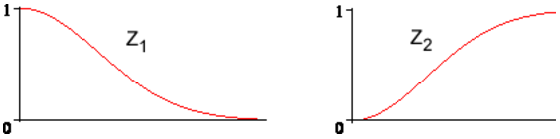
\includegraphics[scale=0.9]{MappingFunctions.png}
\caption{membership functions}
\end{figure}

\textbf{Negation} is defined as $1-z$.  As a consequence of this, for any concept, $z = 0$ means the \textit{antithesis} of that concept.  For example $Z(young) = 0$ would mean �old�. Another consequence is that the point at $z = 0.5$ is the \textit{point of neutrality}, which is where a concept is neither true nor false.

Some concepts (such as ``chair'', ``absurd'') do not have natural opposites.  For these concepts, $z = 0$ means the \textit{complete absence} of the qualities in question.

%Naturally opposite concepts can be represented by 2 predicates, $Q^+$ and $Q^-$, with $z$ values joined at 0 in the middle:
%\begin{table}[H]
%\hspace*{4cm} 
%\begin{tabular}{c c c}
%{\bfseries $z^+ = 1$} & {\bfseries $z^+ = z^- = 0$} & {\bfseries $z^- = 1$}\\
%\multicolumn{3}{c}{$|$\textemdash\textemdash\textemdash\textemdash\textemdash\textemdash\textemdash+\textemdash\textemdash\textemdash\textemdash\textemdash\textemdash\textemdash$|$}\\
%hot       & room temperature & cold\\
%masculine & unisex           & feminine\\
%pretty    & average looks    & ugly\\
%young     & middle age       & old
%\end{tabular}
%\end{table}

Negation can cause some confusion because ``not young'' can mean either ``middle age'' or ``old''.  The only treatment of fuzzy negation that is entirely consistent with our common-sense is to distribute probabilities over fuzziness,  which will be developed after \S\ref{sec:P(Z)-defined}.

The interpretation of the parameter $\xi$ in eqn (\ref{eqn:Z-squashing-fns}) is that it marks the \textit{point of neutrality} on the x-axis, for which z=0.5.  This is illustrated as follows:  we map the human age $x$ to the $\catZ$-concept of ``young'', where I (subjectively) define ``40 years old'' as the neutral point of ``young'':
\begin{figure}[H]
\centering
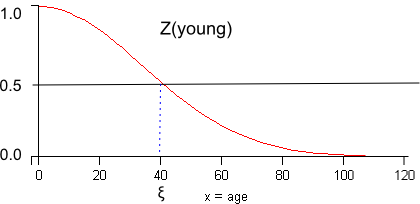
\includegraphics{neutral-point.png}
\caption{neutral point}
\end{figure}
This means, after 40, one gets more and more ``not young'' according to this definition.  

Thus the numerical scale of $\catZ$ is:\\
\begin{table}[H]
\parbox{3cm}{\caption{}}
\begin{tabular}{|l||l|}
\hline
{\bfseries z} & {\bfseries interpretation}\\ \hline
1.0     & definitely or extremely\\
0.9     & very\\
0.7-0.8 & moderately\\
0.6     & slightly\\ \hline
0.5     & neutral\\ \hline
0.4     & slightly not\\
0.3-0.2 & moderately not\\
0.1     & very not\\
0.0     & definitely not\\ \hline
\end{tabular}
\end{table}

Note:  A question has been raised whether we can define opposite concepts with 2 predicates, $Q^+$ and $Q^-$, with $z^+$ and $z^-$ joining at 0 in the middle.  This is not entirely satisfactory because the negation of $Q^+$ would not \textit{cover} $Q^-$, nor vice versa.  Therefore, the choice of $z=0.5$ as neutrality point is quite essential.

\section{Why Z obeys min-max calculus}
\label{sec:min-max-VS-sum-product}

Probabilities obey sum-product calculus;  $\catZ$ obeys \textbf{min-max calculus} \citep*{Zadeh1965}, ie:
\begin{eqnarray}
z_1 \Zand z_2    & \defeq &  min(z_1, z_2) \\
z_1 \Zor   z_2    & \defeq &  max(z_1, z_2).
\end{eqnarray}
My justification for min-max is as follows:

As an example, consider the statement:\\
\hspace*{1cm} S1: \textit{``John have had sex with 1000 women''}\\
but it turns out that all those women had only had cybersex with him.  Most people would agree that cybersex is not quite the same as real sex (some may say it's a borderline case ($z=0.5$)).  Suppose we subjectively think that cybersex is 0.7 real sex (as a measure of degree), then what would be the ``degree of truthfulness'' of the statement S1 (assuming that we accept the fact that he had cybersex with 1000 women)?

If we use the sum-product calculus (as with probabilities), the answer would be $ 0.7^{1000} $ which is almost zero.

Whereas if we use the min-max calculus, the answer would be $min\{0.7, 0.7, ...\} = 0.7$.  So, did John have sex with 1000 women?\\
\hspace*{1cm} answer A:  ``Of course not.''\\
\hspace*{1cm} answer B:  ``Well... sort of.''\\
My view is that the conjunction of 1000 vague events should have the same vagueness as the individual events.  You may try this with other examples of graded events.

%If this is still unclear, consider more examples:\\
%\hspace*{1cm} S2: ``John ate 100 hotdogs in 1 hour'' (but they are all mini-hotdogs)\\
%\hspace*{1cm} S3: ``John defeated 20 chessmasters'' (but they each offered him 2 free moves)\\
%\hspace*{1cm} S4: ``John is fluent in 20 languages'' (but they are computer programming languages)\\
%\hspace*{1cm} S5: ``John finished reading 50 novels'' (but they are all abridged versions)\\
%Would you accept these statements as \textit{partially} true?  Min-max calculus would grant that they are ``somewhat'' true.  Sum-product, however, would infer that they are effectively completely false.

\section{Axiomatic description}
\label{sec:fuzziness-axioms}

In summary, $\catZ$ is the relaxation of the classical-logic view that a statement is either true or false;  {true, false} is relaxed to [0,1].

Here is a set of axioms that describes $\catZ$:

Z1. $z \in [0,1]$ \\
Z2. $z$ varies continuously within $(0,1)$ \\
Z3. $z=0.5$ is the point of neutrality\\
Z4. $\catZ$ obeys min-max calculus when applied by logic conjunction and disjunction

The meaning of Z2 is yet to be clarified.  For now I'd just state it informally.  Also, it would be nice to formulate $\catZ$ calculus in a way similar to Cox's postulates for probabilities, but that is not my current priority.

\section{A fuzzy paradox}

A common problem in fuzzy logic is concerning the truth value of statements such as ``Q and not Q''.  It can be resolved using our understanding of $\catZ$ negation:

Suppose $Z(tall(john)) = 0.6$ (which means that John is slightly tall)\\
then\\
\hspace*{1cm} $ tall(john) \Zand \neg tall(john) = 0.4$ (which means this is slightly false)\\
\hspace*{1cm} $ tall(john) \Zor \neg tall(john) = 0.6$ (which means this is slightly true)

On the other hand, if $Z(tall(john)) = 0.4$ (which means that John is slightly short)\\
then\\
\hspace*{1cm} $ tall(john) \Zand \neg tall(john) = 0.4$ (which means this is slightly false)\\
\hspace*{1cm} $ tall(john) \Zor \neg tall(john) = 0.6$ (which means this is slightly true)

All these are reasonable conclusions.

\section{Unifying AND and OR}
\label{sec:unifying-AND-and-OR}

We seek to unify AND and OR by using a single operator $\varodot$ with a parameter $\theta$ such that when $\theta = 0$ it reduces to AND and when $\theta = 1$ it becomes OR.

A simple way to define $\varodot$ is:
\begin{equation}
X_1 \bigodot_\theta X_2 = (1-\theta) (X_1 \Zand X_2) + \theta (X_1 \Zor X_2).
\end{equation}

The animation (Figure \ref{movie:unified-AND-OR}) shows the graph of $X_1 \varodot X_2$ as $\theta$ varies.

\begin{figure}[H]
\centering
\includemovie[
  poster,
  text={\small(** Click to play **)}
]{200px}{200px}
{unified-AND-OR.swf}
\caption{Graph of $X_1 \varodot X_2$ as $\theta$ varies.\\
\scriptsize{You need to have a PDF viewer that supports Flash, such as Adobe Reader.\\
Make the Reader trust this document.\\
For maximum pleasure click the "play" and "loop" options.}}
\label{movie:unified-AND-OR}
\end{figure}

\section{``Soft'' min-max and concept learning}

\{ TO-DO:  I have some doubts about this section; the argument is a bit unclear.  Maybe soft min-max are unnecessary afterall... \}

As an example, these are 2 exemplars of ``chair'' that most people consider to be typical:
\begin{figure}[H]
\centering
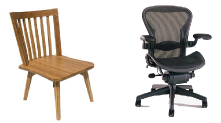
\includegraphics{2-chairs.png}
\end{figure}
Usually, the old-fashioned chair is 4-legged and is made of wood; and the office swivel chair can rotate and has wheels.  These are the \textbf{sfeatures} of the exemplars stored in memory.  It would be atypical for a wooden chair to have wheels and have a seat that can rotate above the 4 legs.  So, even though both chairs are very typical chairs, their features cannot be exchanged freely while maintaining the same level of typicality.

\hspace*{1cm} \begin{tabular}{|l|l|l|} \hline
\textbf{features}            & \textbf{degree} &\\ \hline
wooden $\Zand$ 4-legged     & 1.0             & typical old-fashioned chair\\
rotating $\Zand$ has wheels & 1.0             & typical office chair\\
has wheels $\Zand$ 4-legged & 0.9             & atypical chair\\
\hline
\end{tabular}

It seems that crisp min and max cannot represent this (but I may be mistaken about this point).  Anyway, I created a ``soft'' version of min-max (the idea is to use $z_1, z_2$ as their own weights in a weighted average):

\hspace*{1cm} \begin{tabular}{|l|l|}
\hline
{\textbf{soft min (= AND)}} & {\textbf{soft max (= OR)}}\\ \hline
\rule[-7mm]{0mm}{16mm} 
$\displaystyle z_1 \; \widetilde{\wedge} \; z_2 = \frac{z_1 (1-z_1) + z_2 (1-z_2)}{1 - z_1 + 1 - z_2} $
& $\displaystyle z_1 \; \widetilde{\vee} \; z_2 = \frac{z_1 z_1 + z_2 z_2}{z_1 + z_2} $ \\
\hline
\end{tabular}
\parbox{4cm}{\begin{equation}
\label{eqn:soft-min-max}
\end{equation}}

It can be verified that soft- min and max satisfy the boundary conditions of classical logic, provided that we make $0/0 = 1$ in the min case.

\begin{figure}[H]
\centering
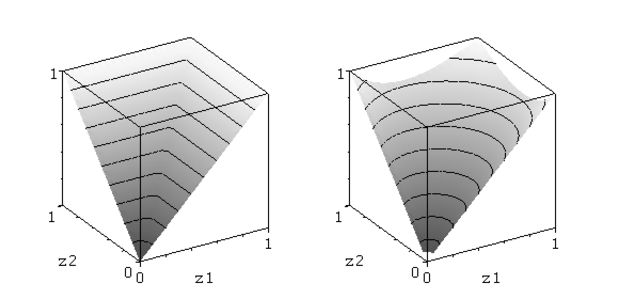
\includegraphics[scale=0.9]{soft-max.png}
\caption{comparison of max and soft max}
\end{figure}

\section{$\catZ$ modifiers}
\label{sec:Z-modifiers}

To make $\catZ$ logic more versatile, we need to augment it with \textbf{modifiers} which correspond to natural-language hedges like:\\
\hspace*{1cm} extremely \hspace*{1cm} very \hspace*{1cm} moderately \hspace*{1cm} slightly\\
so we can express things like:\\
\hspace*{1cm} $\mbox{lukewarm} \leftarrow \mbox{moderately(warm)}$\\
\hspace*{1cm} $\mbox{obese} \leftarrow \mbox{very(fat)}$

In general, we can define a $\catZ$-modifier as a function $\Gamma: [0,1] \rightarrow [0,1]$,
\begin{equation}
z_0 := \Gamma(z_1)
\end{equation}
We further restrict the class of $\Gamma$ to make the system simpler.  I suggest to use Gaussian functions with the mean $z^*$ as a parameter, and the variance would be fixed to a certain constant.  So
\begin{equation}
z_0 := \Gamma(z_1; z^*) = \frac{1}{\sigma \sqrt{2 \pi}} e^{- (z_1-z^*)^2 / 2 \sigma^2}
\label{eqn:fuzzy-moderator-Gaussian}
\end{equation}
For example, the $\Gamma$'s for ``slightly'' and ``very'' can be:
\begin{figure}[H]
\centering
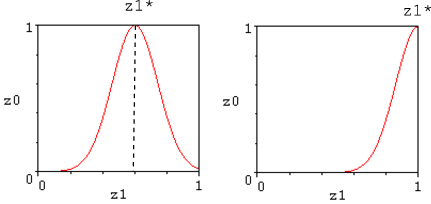
\includegraphics[scale=0.9]{fuzzy-modifiers.png}
\caption{Fuzzy modifiers with $z^* = 0.6, 1.0$}
\end{figure}

We can have better control over the shapes of $\Gamma$ by using other functions and having more parameters, but I suspect that such sophistication is not needed for common-sense reasoning.

For example, we can define ``lukewarm'' as ``warm'' with $z \in [0.6,0.8]$, or:\\
\hspace*{1cm} $\mbox{lukewarm} \leftarrow \Gamma_{0.6}(\mbox{warm}) \Zand \Gamma_{0.8}(\mbox{warm})$\\
using 2 $Gamma$'s with fixed variances.  The result is the blue curve on the left.  We get the interval [0.6,0.8] by taking $> 0.5$ as true, and thus ``lukewarm'' would be a binary predicate.
\begin{figure}[H]
\centering
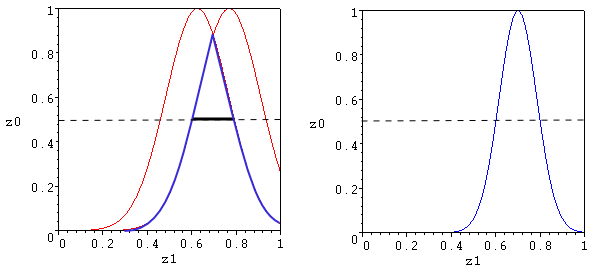
\includegraphics[scale=0.9]{Gamma-for-lukewarm.png}
\caption{Two representations of ``lukewarm''}
\end{figure}
On the other hand, if we use a tailored $\Gamma$ to represent ``lukewarm'' on the right, it would be a $\catZ$-predicate with continuous values like ``slightly lukewarm'' and ``very lukewarm''.  This seems to be unnecessarily sophisticated.

\{ TO-DO:  One problem with this method is that the predicate ``lukewarm'' changes abruptly at the boundaries.  Another example is ``middle-aged''.  \}

\{ TO-DO:  Prove that combinations of $\Gamma$ and $\Zand ,\; \Zor$ can be universal approximators. \}

\section{$\catZ$-conditionals}
\label{sec:Z-conditionals}

In general, inference is driven by rules.  In $\catZ$ logic all rules take the form of $\catZ$-conditionals.  A $\catZ$-conditional is specified by a combination of min's and max's (similar to DNFs (disjunctive normal forms) in classical logic):
\begin{equation}
z_0 \; := \; \bigZor_i \; \bigZand_j \; \Gamma(z_{ij})
%z_0 \; := \; \widetilde{\bigvee_i} \; \widetilde{\bigwedge_j} \; \Gamma(z_{ij}; z^*_{ij}, v_{ij}) \, = \; \widetilde{\bigvee} \; \{ z_{11} \, \widetilde{\wedge} \, z_{12} \, \widetilde{\wedge} \cdots, z_{21} \, \widetilde{\wedge} \, z_{22} \, \widetilde{\wedge} \cdots, \, \cdots \}
\end{equation}

Notice that a $\catZ$ rule directly assigns a $\catZ$ value to $z_0$ \textit{without the use of an implication operator}, which is very different from traditional fuzzy logics:

\subsection{Traditional fuzzy logic}

A fuzzy implication is a map $\Rightarrow: [0,1] \times [0,1] \rightarrow [0,1]$ satisfying these boundary conditions from binary logic:\\
\hspace*{1cm} \begin{tabular}{|l|l|l|} \hline
$\Rightarrow$ & 0 & 1\\ \hline
0             & 1 & 1\\
1             & 0 & 1\\ \hline
\end{tabular}

A fuzzy implication statement:  $(Z_1 \Zand Z_2) \Rightarrow Z_0$  means that the fuzzy values $z_0,z_1,z_2$ obey the equation:
$$ ((z_1 \Zand z_2) \Rightarrow z_0) = z_c $$
where $z_c$ is the truth value of the implication statement.  Compared to my approach, this has an extra level of indirectness.  Is it really necessary that we know the truth value of an implication statement?  (Cf \S\ref{sec:P-and-ClassicalLogic}: In probabilistic logic, the probability conditional $P(A|B)$ serves as the implication statement, but we usually do not ask about its own probability.)  One trouble with traditional fuzzy logic is that we cannot even perform \textit{modus ponens} unless we allow interval fuzzy values.\footnote{Suppose we define the operators for a very simple fuzzy logic: $a \Rightarrow b \equiv \neg a \vee b$, $\neg a \equiv 1-a $, and $a \vee b \equiv min(a,b)$.  \citep*{Kenevan1992} has given an inference algorithm for this logic, but it is very complicated and involves interval fuzzy values, and so is not very suitable for further complex development.}

% Now given that $Z_1 = z_1$ and $Z_1 \Rightarrow Z_0$, ie $ (z_1 \Rightarrow z_0) = z_c $, ie $min(1-z_1,z_0)=z_c$ we still cannot determine $z_0$.}

% TO-DO:  weighted soft min-max may not be needed, if we have fuzzy modifiers

%An example involving vagueness: ``smart''\\
%\hspace*{1cm} smart $\leftarrow$ humorous\\
%\hspace*{1cm} smart $\leftarrow$ articulate\\
%\hspace*{1cm} smart $\leftarrow$ blah

\section{Combining $\catB$, $\catP$, $\catZ$}
\label{sec:combinePZ}

\subsection{The truth value P(Z)}
\label{sec:P(Z)-defined}

How to combine $\mathcal{P}$ and $\catZ$?  The answer is simple because there is no other choice:  the semantics of probabilities dictate that $\mathcal{P}$ must be \textit{distributed over events}.  In the current system, events are either $\mathcal{B}$ or $\catZ$ (the latter are \textit{continuous} events).  So we \emph{distribute $\mathcal{P}$ over $\mathcal{B}$ and $\catZ$}.  In this sense, fuzziness is more fundamental than probabilities.

If a $\catZ$ value is uncertain --- for example, we may not be sure how tall Mary is (the $\catZ$-value of her tallness may be 0.6-0.8, say, so we can assume a uniform probability distribution over the interval [0.6,0.8] which is the green rectangle below) --- and we can approximate it by a Beta distribution over $\catZ$ with a mean at 0.7 and the same variance:
\begin{figure}[H]
\centering
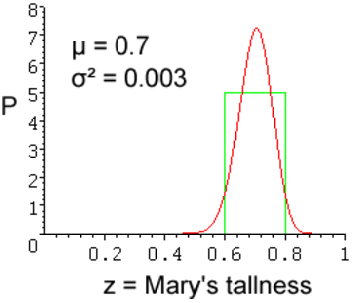
\includegraphics[scale=0.9]{P-over-Z-Marys-Tallness2.png}
\caption{an example $\mathcal{P}(\catZ)$ distribution}
\end{figure}
where the probability density should sum to 1: $ \int^1_0 P(z) dz = 1 $.

On the other hand, if a $\mathcal{P}$ value is uncertain, we simply \textit{ignore} its error (eg, by choosing the mid-point of a P-interval).  \S\ref{sec:PointValued} tried to justify this.

The following commutative diagram shows the relationship between $\mathcal{B}$, $\mathcal{P(B)}$, $\catZ$, and $\mathcal{P(Z)}$:

\begin{figure}[H]
\centering
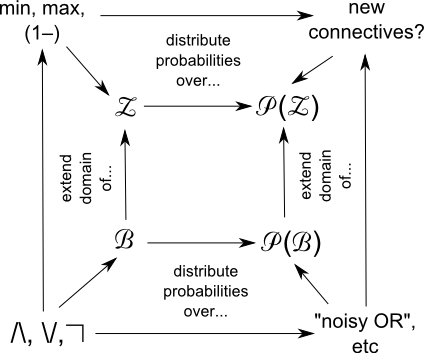
\includegraphics[scale=0.8]{P(Z)-commutative-diagram.png}
\end{figure}

The inner square contains the 4 types of truth values.  The outer square are the corresponding logics, showing their logical operators.  The radial arrows point to the ``underlying sets'' of TVs.

\subsection{An example}

Consider the common sense notion:\\
\hspace*{1cm} \textit{The richer a person, the more powerful s/he is.}\\
Note that this rule is inexact:  there are exceptions (where some rich people are not powerful and some powerful people are not rich) and deviations (the data points do not fall on a straight line):

\begin{figure}[H]
\centering
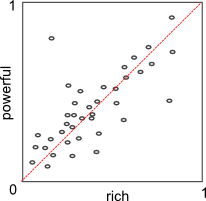
\includegraphics{rich-vs-powerful.png}
\end{figure}

There are reasons to believe that the identity function (red line) represents the least-error regression function:  first, the $\catZ$ values are in ``natural scale'' (ie, $z=1$ corresponds to $\infty$) so $(z_1,z_2)$ at $(1,1)$ is obvious if we accept the original statement;  secondly, when $z_1 = 0.5$, the person is neither rich nor poor, and we should have nothing to say whether the person is powerful or not, as far as the original statement is concerned.

\underconst

\subsection{Unifying all truth values to $\catPZ$}
\label{sec:unifying-P(Z)}

Up to now there are 4 possible TV types:
\begin{table}[H]
\parbox{3cm}{\caption{}}
\begin{tabular}{|l|l|l|} \hline
\multicolumn{3}{|c|}{\textbf{truth values}}\\ \hline
category                   & meaning                                      & definition \\ \hline
$\mathcal{B}$              & binary                                       & $b \in \{true, false\} $\\
$\catZ$              & fuzzy                                        & $z \in [0,1] $\\
$\mathcal{P}(\mathcal{B})$ & $\mathcal{P}$ distributed over $\catZ$ & $ P(b=false) = p_0 $\\
                           &                                              & $ P(b=true) = p_1 $\\
$\mathcal{P}(\catZ)$ & $\mathcal{P}$ distributed over $\catZ$ & $ P(z=z_1) \sim Beta(z_1) $\\ \hline
\end{tabular}
\end{table}
I find that they can be unified to type $\mathcal{P(Z)}$, which can make things simpler.  Below is how to represent the other 3 TV types as $\mathcal{P(Z)}$:

\subsubsection{Type $\mathcal{B}$}

Some variables have a strong ``binary flavor''.  For example, in common sense, a person is either dead or alive, although a more nuanced view will have grades of being dead.  If deadness is a $\catZ$ variable, z = 0 would be ``definitely alive'', z = 1 would be ``definitely dead'' (eg reduced to ash), and z = 0.5 would correspond to a state that is difficult to classify as dead or alive, eg a brain-dead, vegetative state.  z = 0.7 may be a state that is more dead than brain-dead and yet more alive than ash, eg --- I have to pause for a while to think of an example --- a body under cryonic preservation.  And z = 0.4 may be some kind of near-death experience.  Anyway, one can expect the probability distribution of $z_{dead}$ to be polarized with a trough in the middle.  This can be represented by a Beta distribution with a large variance:
\begin{figure}[H]
\centering
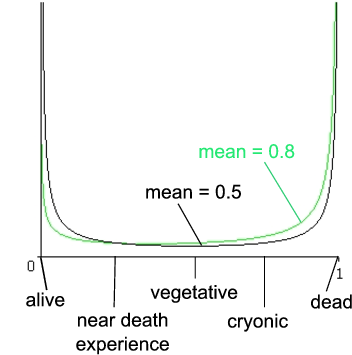
\includegraphics{deadness.png}
%\caption{Z = deadness}
\end{figure}
When the polarization gets extreme (eg the toss of a coin is either head or tail), the distribution becomes a $\bigsqcup$ shape.  The degree of polarization (ie amount of variance) can be estimated statistically, if data is available.

It appears that all common-sensical $\mathcal{B}$ variables are actually \textbf{polarized} $\catZ$ variables.  Another example is a person being either married or not married, and there are grey areas like gay marriage or marriage for the green card, etc.

Actually the Beta distribution (eqn \ref{eqn:beta-distro}) is capable of representing 3 types of characteristics (with $a = 1$ and $b = 1$ as points of transition separating the 3 regimes):
\begin{figure}[H]
\centering
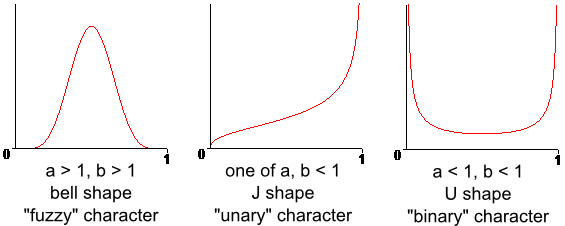
\includegraphics[scale=0.8]{binary-fuzzy-unary-characters.png}
\end{figure}
The unary type represents concepts such as ``normal'', ``broken'', ``healthy'', or ``natural''.  In such concepts, the state at $z = 1$ can be clearly defined (eg, John was perfectly healthy when he was a kid), but as we approach $z = 0$ the cases become very improbable and inexhaustible (eg, it is impossible to find a person who is ``utmost unhealthy'' because it is always possible to think of more extreme and improbable unhealthy ways.  Also, committing suicide is not the limiting case --- suicide is not the same as unhealthy --- so the interval is open-ended.)

\textbf{About the mean and variance.}  In the fuzzy regime, the smaller the variance, the shaper the peak and thus the more confident we are about the $\catZ$ value;  The variance is a measure of confidence in this regime.  In the binary regime, the greater the variance, the more \textit{polarized} the distribution becomes;  The variance is a measure of binary character.  In the unary regime, the meaning of the variance is unclear.

%The transition occurs at $a = 1$ or $b = 1$:
%\begin{figure}[H]
%\centering
%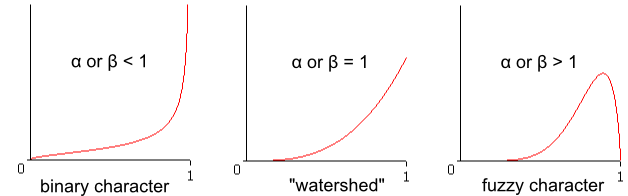
\includegraphics{Beta-distro-watershed.png}
%\end{figure}

%If we know the mean $\mu$, the variance at the transition point is given by:
%\begin{equation}
%v_0 = \frac{(\mu-1)^2 \mu}{2-\mu} \quad or \quad v_1 = \frac{\mu^2(1-\mu)}{\mu+1}
%\end{equation}
%The important thing to understand is that the meaning of the variance is \textit{reversed} after the transition point.  Usually, the variance increases when the sharpness decreases.  But when we have ``binary character'', the distribution gets sharper when variance \textit{increases}, as the probability mass is being pushed to the extremes.  Thus, greater variance here means greater precision.

%Something is wrong here.  There is not one transition point, but a band?  The transition occurs when, giving more variance will give more to the poles.  But this is always true!  So there is no clear cut boundary.  At one extreme is variance = 0, where one of $a, b = \infty$, or when one of $a, b = 0$.  When the variance gets to its maximum, $a = b = 0$ and we have fractional Dirac deltas at the poles, which is fine with the binary interpretation.  The question is when does the binary regime start?  It seems that there is really a transitional band.  It is difficult to say that the J shape is binary or fuzzy.  Examples of J are ``normal'', ``sane'', ``healthy'', ``natural'', etc.  J may be called the ``unary'' regime.

%\textbf{About the mean.}  In the fuzzy regime, the mean is at or near the most probable value, and the variance is a measure of uncertainty about the mean.  In the binary regime, the interpretation is different.  Here, the most probable values are at 0 or 1, and the mean indicates which extreme has higher probability.  The variance indicates the degree of polarization --- the higher, the more ``binary''.

To illustrate this with an example:  In the fuzzy regime, I can say ``John is 0.7 dead because he's in a cryonic state'', and I can use a small variance to indicate that I am confidence that John is in a cryonic state and \textit{not elsewhere}.  In the binary regime, however, I can only indicate the probability of ``John being dead or not'' where ``dead'' is an ``either-or'' condition.  The highest probabilities are concentrated at 1 (``definitely dead'') and 0 (``definitely alive''), and the cryonic state has low probability.  Under this regime there is no way to accentuate (make more probable) the cryonic state --- one can only do so in the fuzzy regime.  This is exactly what we would expect with a binary variable.

%This has consequences when we perform belief revision (\S\ref{ch:belief-revision}), when we need to update variances.

%Once we established that a variable is polarized, what if we then assert its probability?  Eg P(dead) = 0.7?  This is interesting.  Equally interesting, is when we know P(dead) = 0.7, and then assert its polarity.

\subsubsection{Type $\catZ$}

We can create a $\mathcal{P(Z)}$ distribution with a peak around $z$.  The variance depends on how confident we are of the $z$ value.  If unspecified, we can assign a typical variance to it.

\subsubsection{Type $\catPB$}

For example, ``Mary is probably married'', with p = 0.8.\\
ie \hspace*{1cm} $P(married) = 0.8, \quad \quad P(\neg married) = 0.2$.\\

In general, for any $\mathcal{P(Z)}$ variable $Z$, especially in the binary regime, one can set the probability of ``Z'' (viewed as a binary event) to be equal to the probability mass for $z \geq \frac{1}{2}$ which is given by the CDF of the Beta distribution, ie, the regularized incomplete Beta function:
$$ F(x; a, b) = \frac{ B(x; a, b) }{ B(a, b) } = I_x(x; a, b) $$
where $B(x)$ is the incomplete Beta function:
$$ B(x; a, b) = \int^x_0 t^{a-1} (1-t)^{b-1} dt \mbox{.}$$
Thus
$$ P(Z = \mbox{true}) = P(z \ge \frac{1}{2}) = 1 - P(\Zneg Z) = 1 - P(z < \frac{1}{2}) = 1 - I_x(1/2; a, b) $$

The desired mean $\mu$ can be solved from:
\begin{eqnarray}
I_x(1/2; a, b) = p\\
\mu = a/(a+b)
\label{eqn:mean-and-p}
\end{eqnarray}

An interesting observation:  As the variance $v$ increases, it eventually reaches a maximum $v_{max}$ where $a=b=0$ and the Beta distribution is undefined.  From Mathematica experiments, if we keep $ \mu = a / (a+b) $  fixed:\\
$$ \lim_{a,b \rightarrow 0} I_x(1/2) = \mu - 1 $$
This implies that, in the extreme polarized case:\\
$$ p = 1 - I_x(1/2) = 1 - (1 - \mu) = \mu $$

%The mean is related to $p$ by the simple formula (I'm assuming that the real distribution is like the rectangular distribution and therefore I find it's mean):
%
%\mu = \begin{cases}
%1 - \frac{1}{4p} & \quad 1 \geq p \geq \frac{1}{2} \\
%\frac{1}{4(1-p)} & \quad \frac{1}{2} > p \geq 0
%\end{cases}
%\label{eqn:mean-and-p}
%\end{equation}

The variance represents the degree of polarization of the variable, which varies from one variable to another, and can be quite arbitrary if unspecified.

%The inverse of eqn (\ref{eqn:mean-and-p}) is (with an extension to cover extremes):
%\begin{equation}
%p = \begin{cases}
%1                  & \quad \mu > 0.75 \\
%\frac{1}{4(1-\mu)} & \quad 0.75 \geq \mu \geq 0.5 \\
%1 - \frac{1}{4\mu} & \quad 0.5 > \mu \geq 0.25 \\
%0                  & \quad 0.25 > \mu
%\end{cases}
%\label{eqn:mean-to-p-conversion}
%\end{equation}

Inference of $\mathcal{P(Z)}$ logic will be treated in \S\ref{ch:inference}.

%\section{PZ logic formulated as FOL axioms}
%
%In this section I give the complete axioms for PZB logic, expressed in FOL.  That means, a FOL system will have the power of PZB logic when equipped with these axioms.  Thus, this allows us to build an AGI using a FOL inference engine as the core.

%ref1:  truth-value(s1, mean1, variance1)
%ref0:  truth-value(s0, mean0, variance0)
%
%1. How to represent a rule?  eg  bachelor :- male & ~married
%rule-and(bachelor, male, not_married).
%rule-not(not_married, married).
%
%2. How to deduce the TV of s0 given s1?
%retract(ref0).
%truth-value(s0, new-mean, new-variance).

%\section{Outstanding problems}

%1. There will be many factors.  It seems that the structural organization of factors is more important than numerical curve fits.

%2. Often I feel that the numerical values aren't that important at all.  Also I feel that there are many rules that are just B -- for example, $smart \leftarrow creative$.  Even if we have a Z rule, we should be able to talk about the B counterpart.  This is very perplexing... the Z rule may take away the meta-reasoning ability of B rules...?  But the B rule will retain that ability.  Maybe the Z rule can also have the ability of meta-reasoning?  That 'creative' is a component of 'smart'?

%3. The exact form of $P(Z)$ can be irregular, especially when it is given by several factors.

%4. ``Almost P (interpreted as binary)'' is ``close to P (interpreted as Z) $\wedge$ not P (interpreted as binary)''.  So it can be a strictly-B rule with a Z-literal translated to B.  But if the Z-literal is ``not that close to P'' then ``almost P'' may be partially true.  ``Almost P'' can be slightly true, slightly not true, very true etc.  And that seems to depend on the evaluation of ``close to P''.  Because ``close to P'' can be Z, then it seems that ``almost P'' can be Z too.  

%5. The question is whether ``almost P'' is B or Z.  Maybe in various contexts it can be both?  Or may be if it is ``very almost'' then we can as well make it B.  But if it is ``slightly not almost'' then we should make it Z.

%6. The problem now seems to be that we need meta-level intervention to decide what kind of TVs to use.  But the base logic (object-level logic) has difficulty deciding on its own.  This is a problem because the base logic is not well-defined.  We need some simple rules to decide what kind of TVs to use.

%7. It's obvious we need a choice of TVs.  In the ``almost'' case... there is perhaps a distinction between base logic and meta-logic, but this distinction is orthogonal to the choice of TVs.  Maybe there is always a choice of TVs but it is too sophisticated for the base logic?  But somehow the base logic has to make a choice... 

%8. Do rules have ``intrinsic'' TVs for each slot?

%9. Another problem is how to learn B rules *gradually*?  Perhaps we start with P(B) rules and then their P's tend to $\{0,1\}$?  How about Z rules -- do they ever turn into B rules?  Maybe some of the predicates turn binary?

\chapter{Probabilities ($\mathcal{P}$)}
\label{ch:probabilities}
%\begin{flushright}
%[TO-DO: quote]
%\end{flushright}
\minitoc

For an excellent introduction to probabilistic reasoning and Bayesian networks, see Judea Pearl's book \citep*{Pearl1988}.

\section{Why $\mathcal{P}$ is needed}
\label{sec:whyP}

In machine learning it is often necessary to learn facts that are only \textit{contingently true}, such as the fact that ``females often have long hair''.  Learning algorithms typically need to keep track of the frequencies of how often the hypotheses are true, in order to pick the highly probable ones.  So it seems that probabilistic logic should be built into the knowledge representation.

\section{Gaussian and Beta distributions}

One very useful fact for designing AGI is that many quantities that occur naturally in our physical world seem to obey Gaussian distributions.  This follows from the Central Limit Theorem which states that the sum of a large number of independent and identically-distributed random variables is approximately normally distributed.

The upshot of this is that the majority of fuzzy quantities, such as tallness, can be represented using Gaussian distributions.  For example, the height of an unknown woman may have a Gaussian distribution with a mean of ``5 feet 4''.  So we can just use 2 numbers, the mean and variance, to represent the distribution, instead of using a table which takes up more memory.

Since $\mathcal{Z}$ values are defined within $[0,1]$, we can use the Beta distribution which is defined in the unit interval.  It has parameters $a, b$:
\begin{equation}
f(x; a, b) = \frac{x^{a - 1} (1 - x)^{b - 1} }{B(a,b)}
\label{eqn:beta-distro}
\end{equation}
and is a very versatile and flexible distribution.

Sandy Zabell \citep*{Zabell1982} proved that, if we make certain assumptions about an individual's beliefs, then that individual must use the Beta density function to quantify any prior beliefs about a relative frequency \citep*{Neapolitan2004}.

%\begin{figure}[H]
%\centering
%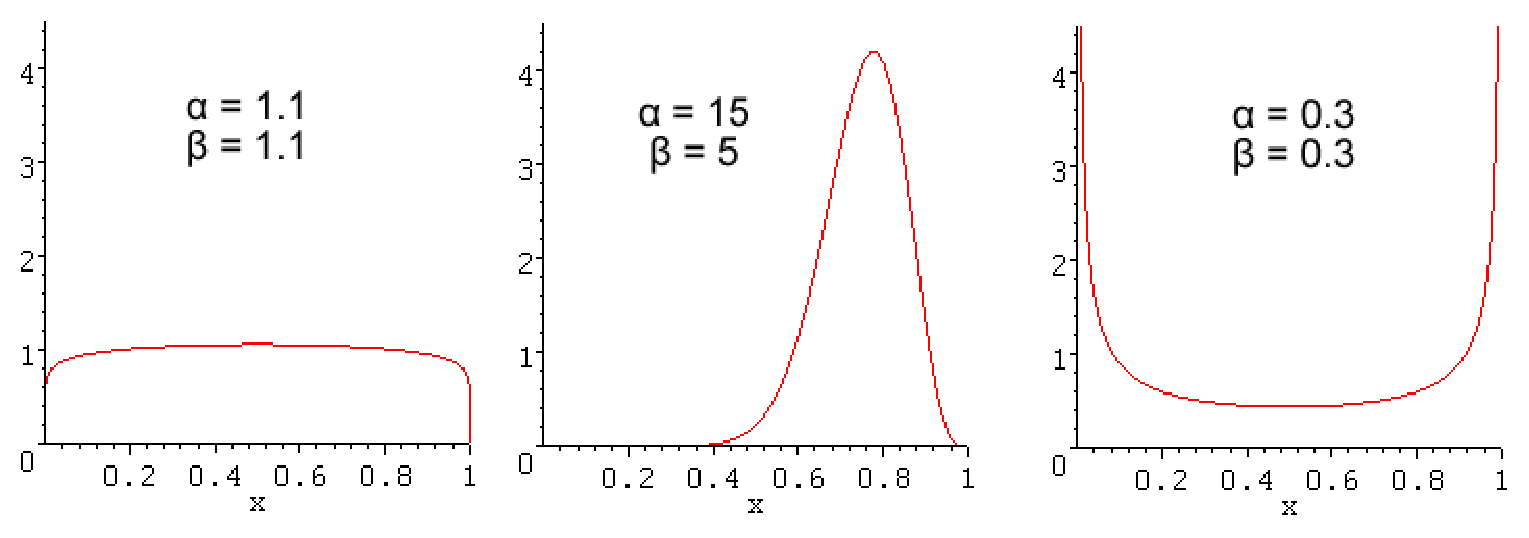
\includegraphics[scale=0.65]{BetaDistributions.eps}
%\caption{some shapes of the Beta distribution}
%\end{figure}

%\begin{enumerate}
%\item The first graph shows an almost uniform distribution, which represents a high amount of uncertainty.
%\item The second graph is unimodal.
%\item The third graph shows a U shape.  As \S\ref{sec:unifying-P(Z)} shows, it is useful for representing variables with ``binary'' character.
%\end{enumerate}

Some characteristics of its shape:\\
1. If $a > 1$ and $b > 1$ the shape is unimodal with the mode at $x = \frac{a - 1}{a + b - 2}$.\\
2. If $a < 1$ and $b < 1$ it is a U shape with an anti-mode at the same point, $x = \frac{a - 1}{a + b - 2}$.\\
3. If $a = b = 1$ it is the uniform distribution.\\
4. If $a = 1$ (respectively $b = 1$) then f(x) has a finite non-zero value at $x = 0$ (respectively at $x = 1$).\\
5. If $(a-1)(b-1) \leq 0$ it is J or reverse-J shaped, without a mode or anti-mode.\\
6. If $a = b$ the pdf becomes symmetric about $x = \frac{1}{2}$.\\
7. If $b > a$ the pdf is skewed to the right, and vice versa.

%The multi-variable version of the Beta distribution is the Dirichlet distribution.

It is very useful that the mean $\mu$ and variance $v$ are given by:
\begin{eqnarray}
 \mu &=& \frac{a}{a + b} \\
 v   &=& \frac{ab}{(a + b)^2 (a + b + 1)}
\end{eqnarray}
and their inverse can be solved (by Maple) to give:
\begin{eqnarray}
 a &=& \frac{m(v + m^2 - m)}{v} \\
 b &=& \frac{(v + m^2 -m)(m - 1)}{v}
\end{eqnarray}
From the above it can be seen that the maximum variance occurs at:
$$ v_{max} = m - m^2 $$
at which point the probability mass is entirely at the poles.

Further discussion about how the Beta distribution represents $\mathcal{P(Z)}$ variables is in \S\ref{sec:unifying-P(Z)}.

\section{Causality}

Three recent books that tackle the problem of causality from an AI perspective are: \citep*{Shafer1996}, \citep*{Pearl2000}, and \citep*{Williamson2005}.  There is also a comprehensive reference \citep*{Beebee2009}.

As \citep*{Koller2009}, Ch 21, explains:  We know that a Bayesian network is directed, but the direction of the arrows do not have to be meaningful.  They can even be anti-temporal.  On the other hand, it is common wisdom that a ``good'' BN structure should correspond to causality, in that an edge $X \rightarrow Y$ often suggests that $X$ ``causes'' $Y$, either directly or indirectly.  Bayesian networks with a causal structure tends to be sparser and more natural.  However, as long as the network structure is capable of representing the underlying joint distribution correctly, the answers that we obtain to probabilistic queries are the same, regardless of whether the network structure is causal or not.


It seems that causal relations cannot be captured simply by probabilistic relations but require some form of inductive algorithm to obtain, such as the IC (for ``inductive causality'') algorithm proposed by \citep*{Pearl2000}.

\underconst

\section{First order logic and Bayesian networks}
\label{sec:FOL-BN}

Early developments in Bayesian network are mainly propositional, which means that each node in a network represents a proposition without variables, such as ``the fact that the alarm sounded''.  It has long been recognized that ``lifting'' Bayesian networks to first order is necessary for AI to be able to deal with open domains where \emph{relations} can be defined over many \emph{objects}.

\begin{figure}[H]
\centering
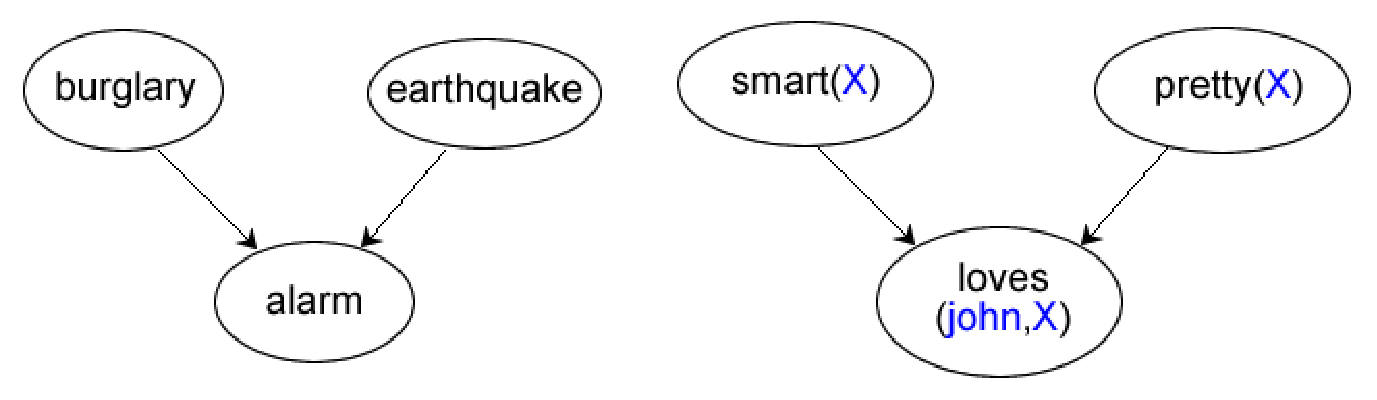
\includegraphics[scale=0.7]{FirstOrderBayesNet.eps}
\caption{propositional vs first-order Bayesian networks}
\end{figure}

One key idea in first-order Bayesian networks is the method of Knowledge-Based Model Construction (KBMC), first developed by \citep*{Wellman1992} and \citep*{Haddawy1994}.  The idea is to store a knowledgebase of first-order rules that can be used to construct propositional Bayesian networks on demand.  When a query is asked, a Bayesian network is generated on-the-fly to answer the query.  This idea helps us think of the first-order case in terms of the propositional case (though it may not be the most efficient implementation in practice).

Also, I have chosen the ``directed'' approach based on Bayesian networks, versus the ``undirected'' approach based on Markov networks (eg \citep*{Domingos2007}'s Markov Logic Network (MLN)).  It seems that the directed approach is more intuitive, in which probabilistic conditionals are used to represent \emph{causal} relations.

See the book \citep*{Getoor2007} for a collection of first-order probabilistic logic approaches.

{\bfseries Some first-order probabilistic logics:}

\citep*{Kersting2000}'s Bayesian Logic Program (BLP)

\citep*{Laskey2006}'s Multi-Entity Bayesian Network (MEBN)

\citep*{Getoor2007a}'s Probabilistic Relational Model (PRM)

\citep*{Milch2007}'s Bayesian Logic (BLOG)

{\bfseries Other first-order probabilistic logics I have not looked into:}

\citep*{Sato1997}'s PRISM

\citep*{Muggleton1996}'s Stochastic Logic Program (SLP)

\citep*{Jaeger1997}'s Relational Bayesian Network (RBN), etc...

\section{Classical logic must give way to Bayesian logic}
\label{sec:P-and-ClassicalLogic}

Now we examine the relation between Bayesian networks and classical logic.

\subsection{Classical implication is ``out''}
The notion of implication in classical logic is no longer applicable in a probabilistic setting.  To see why, consider the classical equivalence of implication\\
\hspace*{1cm} $ A \rightarrow B \equiv \neg A \vee B $\\
and if we try to calculate the probability truth value of this statement we get\\
\hspace*{1cm} $ p = P( \neg A \vee B ) = P(\neg A) + P(B) - P(B|\neg A) P(\neg A) $\\
\hspace*{1cm} = $ 1 - P(A) + P(B|A) P(A) $\\
using 3 basic rules of probabilities:\\
\hspace*{1cm} $ P(X \vee Y) \equiv P(X) + P(Y) - P(X \wedge Y) $  (regardless of whether X,Y are independent)\\
\hspace*{1cm} $ P(X \wedge Y) \equiv P(Y|X)P(X) $\\
\hspace*{1cm} $ P(X) \equiv P(X|Y)P(Y) + P(X|\neg Y)P(\neg Y) $.

Now we have 4 things:\\
\hspace*{1cm} 1.  $ P(A) $\\
\hspace*{1cm} 2.  $ P(B) $\\
\hspace*{1cm} 3.  $ P(B|A) $\\
\hspace*{1cm} 4.  $ P(A \rightarrow B) = P(\neg A \vee B) = p $\\
but they cannot be fixed independently of each other: if we fix any 3 the 4th will also be fixed.

What is the problem here?  The classical implication ``$A \rightarrow B$'' serves a function \textit{similar} to the probabilistic conditional $P(B|A)$, but they constrain probabilities in slightly different ways, so they conflict with each other.  If we keep both copies of \#3 and \#4 in our KB, and apply machine learning to learn their truth values, the values may fail to converge.  It seems that classical implication is only \emph{accidentally} equivalent to $\neg A \vee B$ when things are binary.  In the probabilistic setting, we should jettison the binary implication in favor of the probabilistic conditional.

Adding probabilities to binary logic in a direct way (ie, using the binary material implication instead of $P(B|A)$) will result in very awkward inference algorithms (cf \citep*{Ng1992}, \citep*{Nilsson1986}) that require setting up sets of inequalities for probability bounds.  The result is so awkward that I think for all practical purposes this formulation can be said to be wrong.  The Bayesian network formulation (using conditional probabilities $P(B|A)$) should be preferred.

\textbf{Translating classical logic to Bayesian networks.}  (Note:  this translation is inexact but it preserves the intended meaning informally.)  First, we can translate a first-order KB into Horn form.  This is generally impossible, since Horn logic is a strict subset of first-order logic, but it can be done if we compile the knowledgebase into a pseudo-Horn form and use a special inference algorithm (this is done in \citep*{Stickel1988}).  A Horn formula (which is equivalent to a Prolog statement) having the form:\\
\hspace*{1cm} \texttt{A :- B, C, D, ...}\\
would corresponds to:\\
\hspace*{1cm} $ P(A | B, C, D, ...) = p $\\
in a Bayesian network.  This approach is also adopted by BLP, MEBN, BLOG, and PRM (see \S\ref{sec:FOL-BN}).

\subsection{The probabilistic quantifier ``$\#$''}
\label{sec:probabilistic-quantifier}

In addition to the classical quantifiers $\forall$ (``for all'') and $\exists$ (``exists''), we can introduce a probabilistic quantifier $\#$ (``for some'').  It returns as truth value the probability of the quantified statement.

For example, the truth value of:\\
\hspace*{1cm} \formula{\#x. tall(x)} \hspace*{5cm} ``Some x's are tall''\\
can be defined as:\\
$$ \frac{|\{ x | tall(x) \}|}{| \mbox{reference class of } x |} $$

Notice that the reference class of $x$ cannot be read from the formula above; it must be specified by the \textbf{type} of $x$, such as:\\
\hspace*{1cm} \formula{\#x:human. tall(x)}.

How can the computer know the sizes of these sets?  It seems that it has to keep a record of the sizes every time a new fact is encountered.  For example:\\
When \formula{tall(john:human)} enters the sensory stream, we should note that \formula{john} belongs to the classes \formula{chinese}, \formula{male}, \formula{human}, \formula{organism}, etc.  Each of these reference classes remembers its average tallness (stored as a distribution with its mean and variance, and a confidence, which gives the size of its support).  These records will be updated according as John's tallness compares to the distributions.

In other words, for each property (ie, predicate) we have to record the distributions for (at least) the \underline{typical classes that the predicate applies to}.

\section{Interval-valued probabilities}
\label{sec:intervalP}

Sometimes, Bayesian networks fail to reproduce analogous results in classical logic unless we use interval probabilities.  Consider this example:
\begin{quote}
\emph{China and the US are in conflict. If John sides with the US, he'll be a traitor. If he sides with China, he'll be a loser. Either way, John will be miserable.}
\end{quote}

We can express the premises as conditional probabilities:\\
\hspace*{1cm} $P(\mbox{miserable} \,|\, \mbox{traitor} ) = 0.9$ \\
\hspace*{1cm} $P(\mbox{miserable} \,|\, \neg\mbox{traitor} ) = 0.8$ \\
and we want to query the probability $P(\mbox{miserable})$, but it is unknown whether John is a traitor or a patriot.

This example is exactly analogous to the ``resolution rule'' in classical logic.  The classical inference step is:

\hspace*{1cm} traitor $\rightarrow$ miserable\\
\hspace*{1cm} $\neg$ traitor $\rightarrow$ miserable\\
\hspace*{1cm} --------------------------------\\
\hspace*{1cm} miserable

If we construct a Bayesian network we will have the following CPT (conditional probability table):\\
\hspace*{1cm} \begin{tabular}{|l|l|} \hline
\textbf{traitor} & \textbf{miserable}\\ \hline
true             & 0.9\\
false            & 0.8\\ \hline
\end{tabular}

but we cannot evaluate $P(\mbox{miserable})$ since $P(\mbox{traitor})$ is not known.  This is a problem with point-valued Bayesian networks: \emph{they fail to draw some analogous conclusions of classical logic}.

However, according to probability theory:\\
\hspace*{1cm} $ P(A) = P(A | B) P(B) + P(A | \neg B) P(\neg B) $

Therefore:\\
\hspace*{1cm} $ P(\mbox{miserable}) = P(\mbox{miserable} \,|\, \mbox{traitor}) P(\mbox{traitor}) + P(\mbox{miserable} \,|\, \neg\mbox{traitor}) P(\neg\mbox{traitor}) $\\
\hspace*{1cm} $= 0.9 P(\mbox{traitor}) + 0.8 P(\neg\mbox{traitor}) $\\
\hspace*{1cm} $= 0.9 p + 0.8 (1 - p) $\\
\hspace*{1cm} $= 0.8 + 0.1 p $\\
\hspace*{1cm} $= [0.8, 0.9] $

In other words, if we allow the use of interval probability, we can infer that $P(\mbox{miserable}) = [0.8, 0.9]$ even when we assume that $P(\mbox{traitor}) = [0,1]$ (ie, unknown). Thus we obtain a result analogous to classical resolution.

We need a Bayesian network inference algorithm that can handle this type of deduction, but first we consider an important simplification in the next section.  The final algorithm will be given in \S\ref{sec:P-inference}.

\section{Why point-valued probability is sufficient for AGI}
\label{sec:PointValued}

In my opinion, second-order probability (such as interval probability or the indefinite probability developed by \citep*{Walley1991} and used in \citep*{Goertzel2008}) is an overkill for AGI.  It makes the deduction algorithm very complex, and since the machine learning algorithm is based on deduction and is \textit{even more} complex, the latter problem becomes practically impossible to solve in those settings.  So we must make the deduction algorithm as simple as possible.  Therefore I suggest using only point-valued probability.

In \S\ref{sec:intervalP} I showed that interval probability is needed for some inference steps.  That means the probability P itself is uncertain, and it lies in an interval.  The \emph{exact} algorithm for interval-probability inference requires us to set up the bounds of various probabilities and then invoke linear programming to solve for the probability bounds of the query variable (This method was first outlined by \citep*{Boole1854} and then developed by \citep*{Hailperin1965}, \citep*{Nilsson1986}, \citep*{Ng1992} et al. Recently \citep*{Hansen2000}, \citep*{Jaumard2006} developed faster algorithms for it, but still, the complexity of these algorithms is too much to handle if we want to design learning algorithms based on them.)

What I propose is that whenever we obtain an interval P value, we should convert it to a point value by \emph{taking the mid-point of the interval}.\footnote{We still need inference algorithms that can handle intervals as demonstrated in \S\ref{sec:intervalP}, but the intervals will be instantly converted to point-values after each step. This reduces complexity greatly.}

For example, John may be unable to decide whether the president is smart or dumb.  He may ascribe $P = [0.2,0.8]$ to the atom $smart(president)$.  According to my scheme, he can use \[ P = (0.2 + 0.8) / 2 = 0.5 \] as a compromise.  This is like saying ``there's 50-50 chance''.  Is this approximation too bad?  It seems that many people think like this anyway.  I'd be surprised if the human brain maintains 2nd-order probabilities internally.

Moreover, the exact values of P often do not affect our behavior that much.  There is evidence that taking the centroid (the center of mass of a belief distribution) can yield reasonably good results in second-order probabilistic decision-making (\citep*{Sundgren2006}).  Also, \citep*{Bier1993} shows that there are broad classes of utility functions for which uncertainty is irrelevant under expected utility theory, and only mean values are significant.  \{ TO-DO:  There is hand-waving here. \}

Maybe in a much more advanced AGI, we would want 2nd-order precision, but that seems not to be the right priority now.  It may be more effective for an AGI to improve its decisions by:\\
\hspace*{1cm} 1. considering more factors;\\
\hspace*{1cm} 2. updating probabilities using more evidence;\\
\hspace*{1cm} 3. refining explanations (causal relations);  etc.

Using point-valued probabilities (without knowing their error) is not such a big sin, if we compare this with what we do in fuzzy logic all the time.  A fuzzy statement such as:\\
\hspace*{1cm} ``John is fairly tall''\\
is often represented simply by:\\
\hspace*{1cm} tall(john) \hspace{0.5cm} $z = 0.7$\\
which is analogous to representing the probabilistic statement\\
\hspace*{1cm} ``John is usually punctual''\\
with a point-valued probability:\\
\hspace*{1cm} punctual(john) \hspace{0.5cm} $p = 0.8$.

If fuzziness is a more fundamental phenomenon in our knowledge representation, we should be making more fuss about fuzziness than probabilities.  It seems that we ascribe more ``prestige'' to probability theory merely because of psychological reasons.

\section{Probabilistic AND and OR}
\label{sec:probabilistic-AND-OR}

Specifying the CPT (conditional probability table) of a single node of a Bayesian network, if the node has $n$ parents, would require $2^n$ entries.  The ``noisy'' AND and OR gates are designed to simplify this by reducing the number of independent entries to $n$.  The interpretation of the noisy OR gate is that each parent variable $X$ is associated with an ``inhibition probability'', $q$ (\citep*{Pearl1988} p184-187 or \citep*{Russell2003} p500-501).  This is the textbook definition of noisy OR (and I created noisy AND by applying DeMorgan's law\footnote{That is, to require $\overline{X_1 \curlyvee X_2} \equiv \overline{X_1} \curlywedge \overline{X_2}$ and $\overline{X_1 \curlywedge X_2} \equiv \overline{X_1} \curlyvee \overline{X_2}$ }):

\hspace*{1cm} \begin{tabular}{|l|l||l||l|} \hline
\multicolumn{2}{|c||}{} & {\textbf{noisy AND}}           & {\textbf{noisy OR}}\\ \hline
$X_1$ & $X_2$           & $X_1 \curlywedge X_2$          & $ X_1 \curlyvee X_2 $\\ \hline
0     & 0               & $ 1 ? $                        & $ 0 $\\
0     & 1               & $ 1 - q_1 ? $                  & $ 1 - q_1 $\\
1     & 0               & $ 1 - q_2 ? $                  & $ 1 - q_2 $\\
1     & 1               & $ 1 - q_1 - q_2 + q_1 q_2 ? $  & $ 1 - q_1 q_2 $\\ \hline
\end{tabular}

It seem that this definition of noisy AND is problematic (for example, the ``1'' there should be close to 0).

\{ TO-DO:  Abram Demski pointed out that the textbook definition of noisy-OR is actually OK and there is no need to invent a new one. \}

Anyway, I defined my version of ``probabilistic'' AND and OR so that they obey DeMorgan's laws.  Each variable is attached with a ``causal strength'' $c \in [0,1]$, such that when $c \rightarrow 1$ they reduce to classical AND and OR.

It is better to write the complement $(1 - c)$ as superscript.  So the pair $c_l, (1 - c_l)$ is written as $\vec{c}^i = c_i^0, c_i^1$.  In this notation my definitions can be expressed simply as:
\begin{eqnarray}
 X_1 \curlywedge X_2 & = & \sum_{i j} \; ( \vec{c}^i_1 \, \vec{c}^j_2 \, \vec{x}^i_1 \, \vec{x}^j_2 ) \\
 X_1 \curlyvee   X_2 & = & \sum_{i j} \; ( ( \vec{c}^i_1 + \vec{c}^j_2 - \vec{c}^i_1 \, \vec{c}^j_2 ) \; \vec{x}^i_1 \, \vec{x}^j_2 )
\end{eqnarray}
which can be easily generalized to $n > 2$.  When expanded, they yield the following table:

\hspace*{1cm} \begin{tabular}{|l|l||l||l|}
\hline
\multicolumn{2}{|c||}{} & {\textbf{probabilistic AND}} & {\textbf{probabilistic OR}}\\
\hline
%\rule[-3mm]{0mm}{8mm}
$X_1$ & $X_2$ & $X_1 \curlywedge X_2$          & $X_1 \curlyvee X_2$\\ \hline
0     & 0     & $(1-c_1) (1-c_2)$              & $1 - c_1 c_2$\\
0     & 1     & $(1-c_1) \; c_2$               & $1 - c_1 + c_1 c_2$\\
1     & 0     & $c_1 \; (1-c_2)$               & $1 - c_2 + c_1 c_2$\\
1     & 1     & $c_1 \; c_2$                   & $c_1 + c_2 - c_1 c_2$\\
\hline
\end{tabular}
\parbox{8cm}{\begin{equation}
\label{eqn:probabilistic-AND-OR}
\end{equation}}

A CPT can be defined by a combination of probabilistic AND-OR's:
\begin{equation}
X_0 := \bigcurlyvee_i \; \bigcurlywedge_j \; X_{ij}
\end{equation}
where the $X_{ij}$'s are parents of the node $X_0$ in the Bayesian network.

Notice that in the above equation, each connective is associated with a pair of c parameters, so the actual equation is:
\begin{equation}
X_0 := \bigcurlyvee_i \; \bigcurlywedge_j \; X_{ij};c_{ij} \; = \bigcurlyvee \; \{ X_{11};c_{11} \curlywedge X_{12};c_{12} \curlywedge \cdots, X_{21};c_{21} \curlywedge X_{22};c_{22} \curlywedge \cdots, \; \cdots \}
\end{equation}
It can be verified that \emph{association} holds as in classical logic, ie:
\begin{eqnarray}
(A \curlywedge B) \curlywedge C & = & A \curlywedge (B \curlywedge C), \\
(A \curlyvee   B) \curlyvee   C & = & A \curlyvee   (B \curlyvee   C),
\end{eqnarray}
a fact that can be exploited for efficient calculation.

It is also possible to use the trick in \S\ref{sec:unifying-AND-and-OR} to combine AND and OR with the parameter $\theta$:
\begin{equation}
X_1 \varodot X_2 = (1-\theta) (X_1 \curlywedge X_2) + \theta (X_1 \curlyvee X_2)
\end{equation}

% TO-DO:  weighted noisy AND-OR may not be needed, because the weights are absorbed into the c's

\chapter{Confidence ($\mathcal{C}$)}
\label{ch:confidence}
%\begin{flushright}
%[TO-DO: quote]
%\end{flushright}
\minitoc

Pei Wang's uncertain logic is particularly elegant.  I adopt two ideas from his theory, explained below, but the way I use those numbers differs slightly from Wang's (cf his book \citep*{Wang2006} which describes an AGI called NARS (Non-axiomatic Reasoning System)).

\section{Positive and negative evidence}
\label{sec:w-positive-and-negative}

In Wang's logic, each statement is attached with 2 numbers:\\
\hspace*{1cm} $w^+$ = number of positive examples\\
\hspace*{1cm} $w^-$ = number of negative examples\\
In an AGI system, they are the number of times a statement is observed to be true or false, respectively.

For example, for the statement\\
\hspace*{1cm} ``if X is female X probably has long hair''\\
the AGI may have observed 70 females with long hair and 30 females with short hair. The total \textbf{support} for the statement would be $(w^+ + w^-) = 100$ examples.

Using a pair of numbers allows us to know the probability of a statement as well as the the number of examples that support that statement. This is very important because some statements may be supported by very few examples and thus are ``weaker'' than statements with more support.

A major advantage of this 2-number approach is that probabilities can be updated by new examples. For example, if the AGI encounters a new female with long hair, it can update the probability easily with $ (w^+ + 1, \;w^-)$. Such updating cannot be done with the single-number representation of probability.

\section{Confidence}
\label{sec:confidence}

Confidence is a concept borrowed from NARS.  In my terminology, the \textbf{support} of a statement is defined as:
\begin{equation}
w = w^+ + w^-
\end{equation}
which is an integer from 0 to $\infty$.

As Pei Wang did in NARS, the confidence $c$ is the value obtained by squashing $w$ into $[0,1]$, using a nonlinear transform such as:
\begin{equation}
 c = \frac{1}{1 + k/w} \hspace*{1.8cm}  \mbox{(Wang's method)}
\end{equation}
or \vspace{-0.3cm}
\begin{equation}
 c = 1 - e^{-ln2 \; \cdot \; (w / k)^2} \hspace*{1.2cm}  \mbox{(my method)}
\end{equation}
\vspace{-0.8cm}

\begin{figure}[H]
\centering
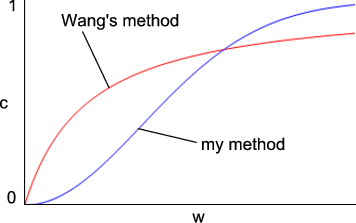
\includegraphics[scale=0.8]{Wang-vs-YKY-confidence-squashing-fn.png}
% \caption{an example $\mathcal{P}(\mathcal{Z})$ distribution}
\end{figure}

An advantage of Wang's method is that it allows statements to have substantial confidence \textit{earlier} (so it gives nascent hypotheses more chance to succeed).  The advantage of my method is that it allows confidence to get closer to 1 sooner (so the incumbents have more strength).  The choice between these 2 may have interesting consequences in machine learning (see \S\ref{sec:confidenceInference}).

\section{Confidence and probability}

The probability (or frequency) of a statement is simply:
\begin{equation}
p = f = \frac{w^+}{w}
\end{equation}
Thus, $(w^+,w^-)$ contains information equivalent to the frequency and confidence pair $(f,c)$.

Notice that the confidence $c$ is \textit{orthogonal} to $f$ or $p$.  In \S\ref{sec:P(Z)-defined} we will see that each truth value in our logic is represented as a tuple: $(\mu, v, c)$ where $(\mu, v)$ describes a probability distribution and $c$ is the confidence.

\section{Confidence and logic}

To see how confidence is defined on logical formulae, it is easier to think in terms of the support $w$.  The support of a \textbf{rule} (ie, a logical formula containing variables) can be defined in a frequentist manner;  whereas the support of a \textbf{ground fact} (ie, a formula without variables) is always \textit{derived} from inference.

For example, the rule:\\
\hspace*{1cm} \textit{``Women usually have long hair''}\\
\hspace*{1cm} female(X) $\rightarrow$ long-hair(X)\\
is supported by a number of instances such as:\\
\hspace*{1cm} positive example: \hspace*{1cm} female(mary), long-hair(mary)\\
\hspace*{1cm} negative example: \hspace*{1cm} female(jane), $\neg$ long-hair(jane)\\
The support of the rule is the \textit{total} number of such instances that have been encountered\footnote{Here the Raven's paradox (or Hempel's paradox) is relevant:  Given the rule that ``women usually have long hair'' we can also state conversely that ``people with short hair are usually not women''.  Thus, a man with short hair would become a supportive example of this rule, which is counter-intuitive.  \{ TO-DO:  resolve this \}}.

A ground fact cannot be given the same treatment because it has no instances (being itself an instance) and its confidence must be inferred.  Inference of confidence is treated in \S\ref{sec:confidenceInference}.

\chapter{Inference}
\label{ch:inference}
\begin{flushright}
\emph{A syllogism has 3 parts; therefore, this is not a syllogism.}
\end{flushright}
\minitoc

By inference we mean deduction and abduction;  induction is regarded a form of learning.

What are the computational bottlenecks?  How to speed things up?

\section{Some background}

\subsection{Resolution}
\label{sec:resolution}

In essence, the resolution rule is:\\
\hspace*{1cm} $P \vee Q $\\
\hspace*{1cm} $\neg P \vee R$\\
\hspace*{1cm} --------------\\
\hspace*{1cm} $Q \vee R$

Resolution is a popular deduction technique for binary logic;  we will not use it but it is helpful to know.

\subsection{Horn clauses and Prolog}
\label{sec:Prolog-Horn-intro}

In essence, a Horn clause is a rule of the form:\\
\hspace*{1cm} \begin{tabular}{l l}
(Prolog notation) &  \texttt{A :- B, C, D, ...}\\
(logic notation)  &  $A \leftarrow B, C, D, ...$
\end{tabular}

The Horn form makes deduction particularly efficient because it is like IF-THEN rules in production systems.  Resolution in Horn form is the basis of Prolog.

\subsection{Forward- and backward- chaining}

These are deduction algorithms.

Forward-chaining \textit{starts with the premises}, and applies deduction steps in the forward direction, to try to arrive at conclusion(s).  A goal (conclusion) may be specified as the search termination criterion;  if not, it is called goal-less forward-chaining.

Backward-chaining \textit{starts with the goal to be proven}, and applies deduction steps in the backward direction.  The search graph terminates with nodes that are the premises.

\subsection{Complexity of inference}

Some facts:

1.  Satisfiability in binary \textbf{first-order logic} is semi-decidable (ie, it terminates in finite time if a proof exists, but may never terminate if a proof does not exist)

2.  SAT for binary \textbf{propositional logic} is NP-complete.

3.  \textbf{Propositional Bayesian network} inference is \#P-complete (ie, it is as hard as returning the number of solutions to an NP-complete problem).

4.  The \textit{naive} algorithm for propositional Bayesian network inference is $O(n 2^n)$ where $n$ is the number of nodes.

5.  Pearl's message-passing algorithm is an \textit{exact} algorithm for propositional Bayesian network inference;  therefore it also requires non-polynomial time in the worst case.

6.  Pearl's algorithm, when operating on trees, is linear time.  But trees seem to be insufficient for AGI reasoning.

7.  SAT for the \textbf{propositional Horn} subclass of binary logic, can be performed in linear time.  My very simple algorithm for Bayesian inference is analogous to Horn deduction\footnote{The term Horn can only be used to describe binary logic:  a Horn clause is a clause with exactly one positive literal.  $\mathcal{PZ}$ logic has a Horn-like form, but the distinction between positive and negative literals disappears in logics with numerical truth values.}.  Prolog owes its efficiency to SLD resolution which is also Horn-based.

\section{Deduction}
\label{sec:deduction}

\subsection{Predicate logic and substitution management}
\label{sec:substitution-management}
\index{substitution!management}

We have argued that propositional (0th-order) logic is inadequate for AGI.  The situation is illustrated as follows:
\begin{figure}[H]
\centering
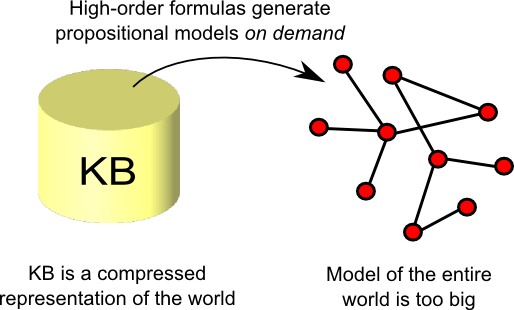
\includegraphics[scale=0.75]{KBMC-illustrated.png}
\end{figure}
This is known as KBMC (knowledge-based model construction).  What it means is that we need to \textbf{fetch} logical rules from the KB and \textbf{instantiate} those rules to form the propositional Bayesian networks upon which probabilities are propagated.
\index{KBMC (knowledge-based model construction)}

Substitution management in first-order logic provers is quite complicated.  This is famously explained in classics such as SICP \citep*{Abelson1984}, where the authors advocated using \textbf{lazy sequences}, also known as \textbf{streams}.

Think of a sequence of \textbf{solutions} attached to each variable node of the proof tree.  Each solution consists of a \textbf{substitution} and a \textbf{TV}.  When we carry out an operation between 2 variables, say $X^1 \varodot X^2$, we are not just dealing with 2 objects, but with 2 \textit{sequences} of possible solutions.  Let's denote the sequences as $X^1 = \{ x^1_1, x^1_2, ... \} $ and $X^2 = \{ x^2_1, x^2_2, ... \}$.  For each solution of each sequence, we need to:
\begin{compactenum}[1.]
\item  Match the 2 substitutions ($x^1_i.\mbox{sub}$ and $x^2_j.\mbox{sub}$), ie, see if they are compatible, and if so, merge the 2 substitutions.\\
       Let's denote the matching operation as $(x^1_i.\mbox{sub} \bowtie x^2_j.\mbox{sub})$.
\item  If the substitutions are compatible, perform the calculation of the CPT (conditional probability table).\\
       Let's denote this operation as $(x^1_i.\mbox{TV} \varodot x^2_j.\mbox{TV})$.
\end{compactenum}
Now denote the combined action of $\bowtie(\cdot, \cdot)$ and $\varodot(\cdot, \cdot)$ as $\heartsuit(x^1_i, x^2_j)$.  Then what we need to calculate can be expressed as:
\begin{equation}
X^0 = \heartsuit( X^1 \times X^2 \times ... \times X^n)
\end{equation}
where $\times$ is Cartesian product, and $\heartsuit$ is extended as an n-ary operation.  Note that each $X^i$ is a (lazy) sequence, so this formula is very succinct.  Further, we can ``curry'' the function $\heartsuit$ so that:
\begin{equation}
\heartsuit \cdot ( X^1 \times X^2 \times ... \times X^n) = (((\heartsuit \cdot X^1) \cdot X^2) \cdot ... )
\end{equation}
where we have made use of the associativity of $\varodot$ (see eqn \ref{eqn:P-and-or-associativity}).  The final RHS is what we will be coding.  It is quite amazing to realize that the proof tree in our program is actually many propositional Bayes nets overlaid together.

\subsection{Pure probabilistic inference}
\label{sec:P-inference}

%The $\mathcal{P}$ inference algorithm is similar to $\mathcal{Z}$ inference (Algorithm \ref{algorithm1}) except that probabilistic inference can be ``abductive'' --- a conditional probability can work in the reverse direction via Bayes theorem --- thus the branching factor of the search would be higher.
%
%\begin{algorithm}
%\caption{backward-chaining P inference}
%\label{algorithm2}
%\begin{algorithmic}[1]
%
%\REQUIRE a knowledgebase $KB$, a list of query goals $G$ \\
%\ENSURE $p =$ probability of $G$.
%
%\REPEAT
%	\STATE choose a literal $L$ from the list $G$, removing it from G
%	\STATE find a rule $X_0 \leftarrow \bigcurlyvee \bigcurlywedge X_{ij} $ such that\\
%			 $L$ unifies with one of the $X_{ij}$'s, including $X_0$\\
%	\COMMENT{ if $X_{ij}$ is null, $X_0$ is a fact in $KB$ }
%	\STATE add the $X$'s to the list $G$, except the one that unifies with $L$ \\
%	\STATE if depth of recursion $< h$ \\
%			 recurse to resolve the new list of goals $G$ \\
%\UNTIL{ there are no more applicable rules in $KB$. }
%
%\end{algorithmic}
%\end{algorithm}

Backward-chaining algorithms in binary logic are relatively familiar to us as they are explained in most AI textbooks.  One of the simplest backward-chaining algorithms is the SLDNF resolution\footnote{SLDNF stands for ``Linear Selection of Definite clauses, with Negation as Failure''.} used in Prolog (see \S\ref{sec:Prolog-Horn-intro}).  Originally I tried to adapt SLDNF resolution for probabilistic inference, but was doing a rather sloppy job of it.  Thanks to Abram Demski who pointed out that my ``Prolog trick'' could actually be replaced with exact Bayesian inference via a technique known as factor graphs, our inference algorithm is now on very good theoretical foundation.
\index{factor graphs}
\index{Bayesian networks!inference}
\index{Bayesian networks!factor graphs}
\index{SLDNF resolution}

TO-DO: There should be a mechanism to prune low-probability (or should it be low-confidence?) branches early on in the search.

%The solution to \#1 is to use 0.5 as the substitute for unknown probabilities.

%The solution to \#2 is to use only local dependencies.

%Case \#1:
%\begin{figure}[H]
%\centering
%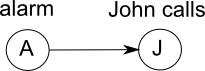
\includegraphics{BayesNet-alarm-John.png}
%\end{figure}
%\textbf{Forward inference}: the answer is simply what is given: $P(J|A)$\\
%\textbf{Backward inference (abduction)}: we seek $P(A|J)$ which is given by Bayes rule:\\
%$$ P(A|J) = \frac{P(J|A)P(A)}{P(J)} $$
%and we search for values of $P(A)$ and $P(J)$; If they don't exist we substitute with 0.5.

%It seems that we need to record the rule during inference.  When the subgoals are all found we can obtain the head.  Is there a way not to store the rules?  No.  Not only that, but we need to have backtrack ability too.

%Case \#2:
%\begin{figure}[H]
%\centering
%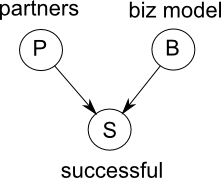
\includegraphics{BayesNet-successful-business.png}
%\end{figure}
%\textbf{Forward inference}: simply given by $P(S|P,B)$\\
%\textbf{Abduction}: given S, we can infer P and B.  "P or B" is a problem. How to represent that?  

\subsubsection{Factor graph algorithm}

Factor graphs are a way to unify probabilistic graphical models such as Bayesian networks and Markov networks.  The important thing to know is that factor graphs are isomorphic to the proof trees we construct during backward-chaining, and thus we can perform Bayesian belief propagation \textit{in situ} in the proof tree, very conveniently.  For example:
\begin{figure}[H]
\centering
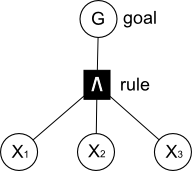
\includegraphics{simple-proof-tree.png}
\caption{Simple proof tree / factor graph}
\end{figure}
In this example we can see that the factor node (black square) is located exactly as the ``rule node'' in the proof tree, therefore we might as well label the node with its operator (``$\wedge$'').

\textbf{The algorithm:}  What we need to calculate, for a "goal" variable node $G$, is $P(G|K)$, where $K$ is the background knowledge.  $P(G)$ is called the prior distribution of $G$.

When the graph has no loops, then it is a tree, and the factor graph algorithm begins from the leaves of the tree to the root which is the goal node.  The leaves pass messages up to their parents, with each factor node performing a \textbf{sum-product} operation, until the messages reach the root.

Assume that we have a rule in the form:
\begin{equation}
H_1, H_2, ... \PimpL X_1 \varodot X_2 \varodot ...
\end{equation}
where the $H$'s stand for ``Heads''.  This is actually a compact way of stating more than 1 rule -- with each head corresponding to 1 rule\footnote{\{ To-do: explain why the multiple-head feature is desirable.\}}.  For simplicity's sake we assume number of $H$'s = 1.  For example:
\begin{figure}[H]
\centering
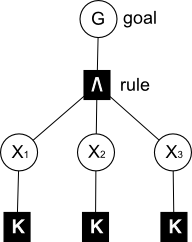
\includegraphics{simple-proof-tree2.png}
\caption{Simple factor graph in ``normal'' direction, with background knowledge}
\end{figure}
The link to $K$ simply means that either the node's value is ``clamped'' or it is passing a message from further down the tree.

In the ``normal'' direction, our $G$ is $H$, so the calculation is pretty straightforward.  From now on we use the notational convention of omitting $P(\cdot)$ for probabilities; ie, $P(X)$ is written as $(X)$:
\begin{equation}
(G|K) = \sum_{X_i} (G|X_i)(X_i|K).
\end{equation}
The first factor on the RHS is the ``\textbf{factor}'' stored in the factor node.  The second factor is the \textbf{messages} coming from each $X_i$ node.  This is a simple sum-product operation.

Next case, the direction is reversed:
\begin{figure}[H]
\centering
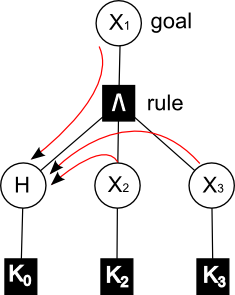
\includegraphics{simple-proof-tree3.png}
\caption{Simple factor graph in backward direction}
\end{figure}
Notice how the rule is not pointing to the goal $G$, and $G$ is now taking the place of $X_1$.  We need to apply Bayes rule twice:

First work out the 2-node case where $X_2, X_3, ...$ don't exist:\\
\begin{eqnarray*}
(G|K) &=& \frac{(K|G)(G)}{(K)} = \frac{(G)}{(K)} \sum_H (K|H)(H|G) \nonumber\\
      &=& (G) \sum_H \frac{(H|K)}{(H)} (H|G)
\end{eqnarray*}

General case:\\
\begin{eqnarray*}
(G|K) &=& \frac{(K|G)(G)}{(K)} = \frac{(G)}{(K)} \sum_H (K|H)(H|G) \nonumber\\
      &=& (G) \sum_H \frac{(H|K)}{(H)} \sum_{X_i} (H|G,X_1,X_2,...)(X_i|G) \nonumber\\
      &=& (G) \sum_H \frac{(H|K)}{(H)} \sum_{X_i} (H|G,X_1,X_2,...)(X_1)(X_2)...
\end{eqnarray*}

\subsubsection{Higher-order Bayesian logic}

Note:  here ``higher-order'' refers to the predicate logic aspect, not higher-order probabilities.

Essentially, what we need to do is to instantiate all possible propositional Bayesian networks with a given goal at the root, when given a set of higher-order formulas in the KB.  (I'm not sure if it is enumerable, but assume that it is.)

In first-order Horn logic, the instantiation procedure seems pretty easy as it follows the SLDNF resolution algorithm (\S\ref{sec:Prolog-Horn-intro}).  With higher-order logic the task is complicated by the fact that variables can instantiate as other formulas.

Our slogan is:  ``One formula -- one Bayesian network link -- one factor graph node.''  Or in symbols:

\vspace{0.1cm} \tab \tab
\fbox{ \parbox{4cm}{
$ \mbox{formula} \equiv \Pimp \equiv \blacksquare $
}}

\{ To-do:  Higher-order unification seems to work fine with such formulas... but I need to work out the details...  \}

\underconst

\subsubsection{Loopy inference}

\underconst

\subsection{Hybrid $\mathcal{B,P,Z}$ inference}

Rules, which are the building blocks of inference, can be of 4 types:

\begin{table}[H]
\parbox{3cm}{\caption{}}
\begin{tabular}{|l|l|} \hline
\multicolumn{2}{|c|}{\textbf{rules}}\\ \hline
mnemonic             & meaning\\ \hline
$\catB$              & Prolog statements of the form\\
                     & \qquad $L_0 \, \mbox{:--} \, L_1, L_2, L_3, ... $ \\
$\catZ$              & Fuzzy rules of the form\\
                     & \qquad $z_0 := \bigZandor \Gamma(z_{ij})$ \\
$\catPB$             & Bayesian network nodes specified by\\
                     & \qquad $X_0 \PimpL \bigPandor X_{ij};c_{ij}$ \\
$\catPZ$             & Specifications of $\catPZ$ distributions\\
                     & \qquad $X_0 := Beta(\mu,\sigma^2)$ \\
\hline
\end{tabular}
\end{table}

The type of a rule is determined by its ``head'' --- eg, if the head is a $\catB$ variable then the rule is a $\catB$ rule.  Using unified $\catPZ$ truth values, we can plug variables of any TV type into any rule.  So, the rule type only affects how the rule is interpreted, which will be explained below.

An example of a rule is:  ``almost Q'' means ``close to Q, but not being Q''.\\
The TV types of the predicates are:\\
\hspace*{1cm} ``almost Q'' --- $\catB$\\
\hspace*{1cm} ``close to Q'' --- $\catZ$\\
\hspace*{1cm} ``not Q'' --- $\catB$\\
So we can represent it with a $\catB$ rule:\\
\hspace*{1cm} $\mbox{almost } Q \leftarrow \mbox{ close-to } Q \wedge \neg Q$
Despite using a $\catB$ rule, the result of inference will be a $\catPZ$ truth value with binary character.  This is a good thing, because the idea of ``almost'' can be fuzzy in some cases, for example:\\
\hspace*{1cm} ``I heard that John almost got killed by the assassination?''\\
\hspace*{1cm} ``Not really, the bullet only hit his toe!''

To simplify things, I consider single inference steps.  A complete proof involves a series of such steps.

\subsubsection{$\catB$ rule:}

The $\catB$ rule can have 3 operators: $\wedge$, $\vee$, and $\neg$.  All we need to do is to show how to evaluate the operators for $\mathcal{P(Z)}$ values.  An example $\catB$ rule is:\\
\hspace*{1cm} \texttt{bachelor :- male $\wedge \; \neg$ married}

Case $\neg$ :  We need to convert the $\mathcal{P(Z)}$ distribution to one with a binary character.  This is done by setting the variance to a fixed value in the binary regime (\S\ref{sec:unifying-P(Z)}).  Then the result is negated by transforming the mean:
\begin{equation}
\mu ' = 1 - \mu
\label{eqn:1-minus-z-transform}
\end{equation}

Case $\wedge$ : Convert the $\mathcal{P(Z)}$ value to $\mathcal{P(B)}$ via eqn (\ref{eqn:mean-and-p}).  Then $P(A \wedge B) = P(A) P(B)$, assuming independence.

The variance is assigned a fixed value so that the resulting variable has binary character.  Note that the resulting variance is not affected by the variances of the premises because the aim of a $\mathcal{B}$ rule is to form a \textit{binary} judgment.

Case $\vee$ : Similar to above, with $P(A \vee B) = P(A) + P(B) - P(A)P(B)$, again assuming independence.

\subsubsection{$\catZ$ rule:}

$\catZ$ rules can have the operators $\Zand$ (= min), $\Zor$ (= max), $\Zneg$ ($= 1-z$) and the fuzzy modifier $\Gamma()$.  At this stage we ignore Soft min and max.  The $\Gamma()$'s are applied before the other operators.

Case $\Gamma$() : If $z_0 := \Gamma(z_1)$ and $z_1$ is given by the probability density function $f_1(z1)$, then the probability density of $z_0$ would be given by:
\begin{equation}
f_0(z_0) = f_1(\Gamma^{-1}(z_0)) \left | \frac{d\Gamma^{-1}}{dz_0} \right |
\end{equation}
which is explained in \citep*{Wikipedia2008}.  If $\Gamma()$ is the Gaussian function given in eqn (\ref{eqn:fuzzy-moderator-Gaussian}) then\\
$$ f_0(z_0) = f_1(\pm \sigma \sqrt{-2 \ln z_0} + z^*) \left | \frac{\sigma}{z_0 \sqrt{-2 \ln z_0}} \right | $$
but there is a glitch:  $\Gamma^{-1}()$ has 2 pieces, and their contributions must be summed up piecewise.  Sometimes the resulting distribution looks irregular, for example:
\begin{figure}[H]
\centering
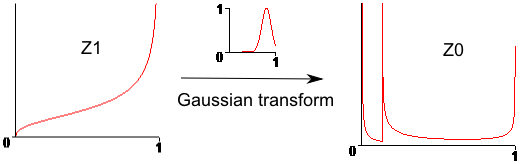
\includegraphics[scale=0.9]{Z1-Gaussian-transform-to-Z0-ugly.png}
\end{figure}
but we can approximate it with a Beta distribution by preserving the mean and variance.  The irregular appearance does not matter that much if we only care about the mean and variance.  I have obtained the approximation formula by numerical integration and nonlinear regression on randomly generated samples, as follows ($m_1$ = mean of input, $m_0$ = mean of result):
\begin{figure}[H]
\centering
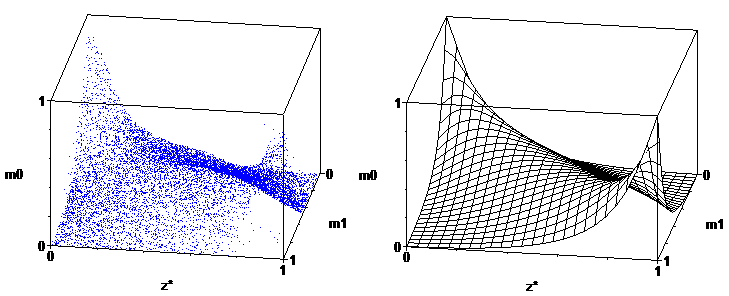
\includegraphics[scale=0.7]{Gaussian-fuzzy-modifier-regression-result.png}
\caption{Gaussian fuzzy modifier:  empirical data and result of regression}
\end{figure}

Case $\Zneg$ :  Simply negate the $\catPZ$ distribution by eqn (\ref{eqn:1-minus-z-transform}) with variance unchanged.

Case $\Zor$ :  Given $z_0 := z_1 \Zor z_2$, ie $z_0 = max(z_1, z_2)$.  What we need to do here is to calculate the PDF of a random variable given as a function of two other random variables.  The procedure is given in many textbooks.

Here $\catP$ denotes probability measure which is a set function, $F(t)$ denotes CDF's, $f(t)$ denotes PDF's.

%Define the region $D_0 := \{ (z_1,z_2): \widetilde{\wedge}(z_1,z_2) \leq z_0 \}$.
%\begin{eqnarray}
%F_0(z_0) & = & \mathbf{P}(Z_0 \leq z_0)\\
%         & = & \mathbf{P}((Z_1,Z_2) \in D_0)\\
%         & = & \iint_{D_0} f_{12}(z_1,z_2) dz_1 dz_2
%\end{eqnarray}
%If we assume $Z_1, Z_2$ independent then $f_{12}(z_1,z_2) = f_1(z_1) f_2(z_2)$.

\hspace*{1.2cm} $ F_0(t) = \mathbf{P}(Z_0 \leq t)$\\
\hspace*{2cm} $= \mathbf{P}(\Zor(Z_1,Z_2) \leq t)$\\
\hspace*{2cm} $= \mathbf{P}(max(Z_1,Z_2) \leq t)$\\
\hspace*{2cm} $= \mathbf{P}(Z_1 \leq t \wedge Z_2 \leq t)$\\
\hspace*{2cm} $= \mathbf{P}(Z_1 \leq t) \, \mathbf{P}(Z_2 \leq t)$ \quad assuming $Z_1, Z_2$ independent\\
\hspace*{2cm} $= F_1(t) F_2(t)$\\
where $$ F_1(t) = \int_0^t f_1(z_1) dz_1 , \quad F_2(t) = \int_0^t f_2(z_2) dz_2$$

%The result we want is: $ f_0(t) = dF_0(t) / dt $
The result we want is:
\[ f_0(t) = \frac{dF_0(t)}{dt} = F_2(t) \frac{dF_1(t)}{dt} + F_1(t) \frac{dF_2(t)}{dt} \]
and we need to apply Leibnitz's Rule.\footnote{For a function of t defined by: $$ F(t) := \int_a(t)^b(t) \Phi(x,t) dx $$ its differentiation is given by Leibnitz's Rule: $$ \frac{dF(t)}{dt} = \int_{a(t)}^{b(t)} \frac{\partial\Phi(x,t)}{\partial t} dx + \Phi(b(t),t) \frac{db(t)}{dt} - \Phi(a(t),t) \frac{da(t)}{dt} $$ }  Then we get:
\begin{equation}
f_0(t) = f_1(t) F_2(t) + f_2(t) F_1(t)
\end{equation}

%If it is $min()$:\\
%\hspace*{1.2cm} $ F_0(t) = \mathbf{P}(\widetilde{\vee}(Z_1,Z_2) \leq t)$\\
%\hspace*{2cm} $\approx \mathbf{P}(min(Z_1,Z_2) \leq t)$\\
%\hspace*{2cm} $= \mathbf{P}(Z_1 \leq t \vee Z_2 \leq t)$\\
%\hspace*{3cm} assuming $Z_1, Z_2$ independent:\\
%\hspace*{2cm} $= \mathbf{P}(Z_1 \leq t) + \mathbf{P}(Z_2 \leq t) - \mathbf{P}(Z_1 \leq t) \mathbf{P}(Z_2 \leq t)$\\
%\hspace*{2cm} $= F_1(t) + F_2(t) - F_1(t) F_2(t)$

This function $f_0$ has an interesting property:  it appears to add up the distributions $f_1$ and $f_2$, \textit{with the one on the right being dominant}, ie, giving the biggest contribution of probability mass (or area under the curve).  Some examples are as follows:
\begin{figure}[H]
\centering
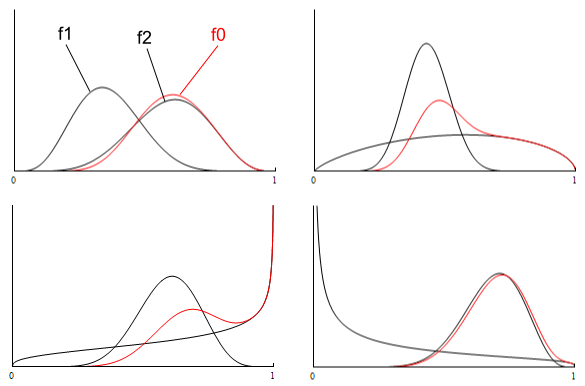
\includegraphics[scale=0.8]{A-ZOR-B-examples.png}
\caption{$z_0 := z_1 \, \Zor \, z_2$}
\end{figure}

%Some observations about the shapes:
%
%A. When the 2 inputs are unimodal:
%
%1. If they are narrow (ie small variance) and fairly separated, the mode on the right almost completely dominates; deviation is negligible.\\
%2. When the 2 modes are close, the mean of the result shifts to the right and variance decreases (the peak gets narrower).\\
%3. If any one input is broad (ie large variance), the result will shift to the right.  The change in variance is ambiguous.
%
%new mean = right mean + (amount of shift)
%amount of shift = f( how close they are, how broad they are)
%if close then new variance = narrower
%
%B. When 1 of the inputs has infinity on one side or both:
%
%1. If infinity is on both sides, the result will retain the infinity on the right, plus a small second peak near the second input (which is shifted slightly to the right).  It may be approximated by a J shape with a or b = 1 on one side.\\
%2. If infinity occurs on the right only (J shape), that infinity dominates the result, and the second input has a rather slight effect.\\
%3. If infinity occurs on the left, the second input will dominate.  Deviation from the second input is very slight.
%
%C. If both inputs have infinities:
%
%1. When 2 J shapes are crossed, the right side dominates, and there is a very slight shift to the left (but the stats seem to indicate that the shift can be big).  Sometimes, but rarely, to the right too -- why? Well the reason can be quite obscure.\\
%2. With a U shape and a J shape to the left, the result is a J shape to the right but with a small peak near the left end.  May be difficult to approximate (or use the power distribution?)\\
%3. With a U shape and a J shape to the right, the result is a J shape to the right with a greater variance (ie more polarized).  The degree of extra polarization depends on the contribution of the U shape (whether it's heavy on the right side).\\
%4. With 2 U shapes, the result is a J shape.

Once again, we approximate by preserving the mean and variance; The irregular appearance is not so important.  By looking at the following graph we can see that the mean of the result ($m_0$) is mostly dominated by $m_2$ which is the mean of the input further to the right (ie, $m_2 > m_1$).  There is sometimes a slight shift to the right relative to $m_2$ (the dots above the $x=y$ line), but it seems insignificant and may be ignored.  In other words, the fuzzy inference rule is very simple:  \textit{the mean of the result is just the greater mean of the 2 inputs}.  A similar graph shows that the variance of the result is also approximately equal to the variance of the rightmost input.
\begin{figure}[H]
\centering
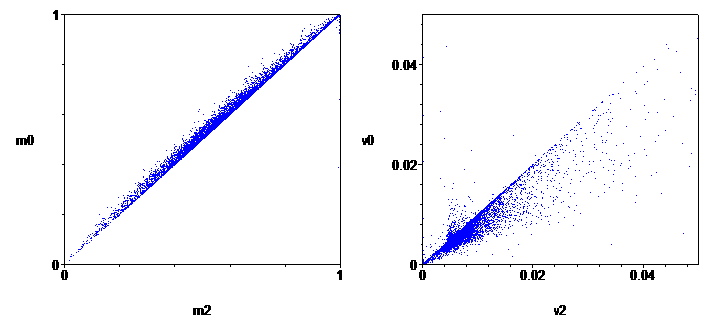
\includegraphics[scale=0.8]{z1-OR-z2-M-and-V-plots.png}
\caption{Plots of mean and variance; output vs input}
\end{figure}

Case $\Zand$ : The result for $z_0 := z_1 \, \Zand \, z_2$ is similar (again assuming $Z_1, Z_2$ independent):
\begin{equation}
f_0(t) = f_1(t) + f_2(t) - f_1(t) F_2(t) + f_2(t) F_1(t)
\end{equation}

In summary, the fuzzy inference rules are:

\fbox{ \parbox{8cm}{
1. For $z_0 := \neg z_1$\\
\hspace*{0.3cm}  $\mu_0 = 1 - \mu_1$\\
\hspace*{0.3cm}  $v_0 = v_1$ \\
2. For $z_0 := z_1 \vee z_2$\\
\hspace*{0.3cm} $\mu_0 = max(\mu_1, \mu_2)$\\
\hspace*{0.3cm} $v_0 = \left\{ \begin{array} {r@{\quad:\quad}l}
					v_1 & \mu_1 > \mu_2\\
					v_2 & \mu_2 > \mu_1 \end{array} \right.$\\
3. For $z_0 := z_1 \wedge z_2$\\
\hspace*{0.3cm} $\mu_0 = min(\mu_1, \mu_2)$\\
\hspace*{0.3cm} $v_0 = \left\{ \begin{array} {r@{\quad:\quad}l}
					v_1 & \mu_1 < \mu_2\\
					v_2 & \mu_2 < \mu_1 \end{array} \right.$\\
4. For $z_0 := \Gamma(z_1)$,
$$ \mu_0 = \frac{k_1+k_2}{\sigma_1} e^{- (m_1-z^*)^2 / \sigma_1^2 } $$
$$ v_0 = \frac{k_3}{\sigma_2} e^{- (z^* - \sqrt{3} m_1 + k_4)^2 / \sigma_2^2 } $$
\hspace*{0.3cm} where $\sigma_1 = k_1 (m_1+z^*-1)^2 + k_2 $ \\
\hspace*{1.4cm}     $\sigma_2 = k_5 (z^* + \sqrt{3} m_1 - k_6)^2 + k_7 $ \\
\hspace*{0.3cm} the $k$'s are regression parameters
}}

\subsubsection{$\catPB$ rule:}

A $\mathcal{P(B)}$ rule is of the form:\\
\hspace*{1cm} $X_0 := \bigPor \bigPand X_{ij};c_{ij}$

To simplify things, we do not implement the Bayesian network algorithm, instead we only perform the calculation $X_0$ from $X_{ij}$ in one direction.  This is an extreme simplification of probability logic, but it may already be sufficient for common-sense reasoning.  We will try this first and see how far it can go.

The $\catPZ$ variables can be converted to $\catPB$ variables via eqn (\ref{eqn:mean-and-p}).  Then the $\catPB$ value of the consequent can be obtained via straightforward application of probabilities, eg:\\
%\hspace*{1cm} $P(X_1 \wedge X_2) = \sum_{i=1,2} P(X_1 \wedge X_2 \; | \; P(X_i)) \; P(X_i)$ \\
\hspace*{1cm} $ P(X_1 \wedge X_2) = (1-p_1)(1-p_2)(1-c_1)(1-c_2) \; + $ \\
\hspace*{3.5cm} $ (1-p_1)p_2(1-c_1)c_2 \; + $ \\
\hspace*{3.5cm} $ p_1(1-p_2)c_1(1-c_2) \; + $ \\
\hspace*{3.5cm} $ p_1 p_2 c_1 c_2 $ \\
where $p_i = P(X_i)$.  Note that it reduces to the binary case when $c_1 = c_2 = 1$.  The result is then converted back as a $\mathcal{P(Z)}$ distribution (with binary character).

\subsubsection{$\catPZ$ rule:}

We do not use truly $\catPZ$ rules because they are too complex and not needed for common-sense reasoning.  The $\catPZ$ rules we have are simpler operations that allow us to manipulate the $\catPZ$ distributions of variables.

We can directly assign the mean and variance to a $\catPZ$ variable:\\
\hspace*{1cm} $X_0 := Beta(z; a, b)$

Or we can fix the probability at a particular point $z*$'s neighborhood.  For example, ``the probability of Mary being 0.9 fat is 0.1''.

%\textcolor{red}{The stuff below this line are just my notes and may contain many errors.}
%\hrulefill

%In the probabilistic setting... we have to deal with adding rules and using the ``combination rule''... 
%
%\hspace*{1cm} \[ f = \frac{f_1 w_1 + f_2 w_2}{w_1 + w_2} \]

%The assumption is...?
%
%The confidence of the result is given by:\\
%\hspace*{1cm} \[ c = C(c_1, c_2) ? \]

%\subsection{Hybrid rules}
%\label{sec:hybrid-rules}
%
%Some rules may involve factors of various truth-value types.  For example, ``almost'' means ``close to, but not being'', which translates to this rule:\\
%\hspace*{1cm} $\mbox{almost } Q \leftarrow \mbox{ close-to } Q \wedge \neg Q$\\
%where the first factor is $\mathcal{Z}$, the second factor is $\mathcal{B}$.
%
%Maybe we should disallow $\mathcal{P}(\mathcal{Z})$-rules in the AGI because they are too sophisticated?
%
%The hybrid rules can be:\\
%\hspace*{1cm} \begin{tabular}{|l|l|l|l|l|} \hline
%                           & $\mathcal{B}$           & $\mathcal{Z}$                     & $\mathcal{P}(\mathcal{B})$ & $\mathcal{P}(\mathcal{Z})$\\ \hline
%                           & $\vee \wedge$           &                                   &            & \\
%$\mathcal{Z}$              & case H1                 & $\widetilde\vee \widetilde\wedge$ &                         & \\
%$\mathcal{P}(\mathcal{B})$ & $\curlyvee \curlywedge$ & case H2                           & $\curlyvee \curlywedge$ & \\
%$\mathcal{P}(\mathcal{Z})$ & case H3                 & case 8                            & case H4                 & $\widetilde\curlyvee \widetilde\curlywedge$ \\ \hline
%\end{tabular}
%
%TO-DO:  unfinished.

%\subsection{Unified $\mathcal{P(Z)}$ rules?}
%\label{sec:unified-BPZ-inference}
%
%This section is optional.  As far as inference goes, the rest of this chapter has outlined the algorithms.  Here we try to see how $\mathcal{B}$, $\mathcal{P}$, and $\mathcal{Z}$ can be unified under the most general logic, $\mathcal{P}(\mathcal{Z})$.  Such a logic may be desirable in machine learning, where the general form of $\mathcal{P}(\mathcal{Z})$-rules may allow us to perform the searching in a continuous space, and some of the rules will degenerate nicely into $\mathcal{B}$, $\mathcal{Z}$, and $\mathcal{P}(\mathcal{B})$ rules.  Anyway, it turns out that $\mathcal{P}(\mathcal{Z})$-rules are not that simple and degeneration is also complex.
%
%First, let's start with a general form of $\mathcal{Z}$-rule which is a function $\mathcal{Z} \times \mathcal{Z} \cdots \rightarrow \mathcal{Z}$:\\
%$$ z_0 := \widetilde{\bigvee_i}\, \widetilde{\bigwedge_j}\, \Gamma_{ij}(z_{ij}) $$
%where $\Gamma_{ij}$ are Gaussian functions with means $z^*_{ij}$ and variances $v_{ij}$ (in other sections we don't use the variance).  The interpretation of $\Gamma$ is:  $z^*_{ij}$ represent the optimal values, which results in $\Gamma = 1$, and when $z_{ij}$ deviates from $z^*_{ij}$, $\Gamma$ drops from 1.
%
%Now generalize this to the $\mathcal{P}(\mathcal{Z})$-rule which is a function $\mathcal{P}(\mathcal{Z}) \times \mathcal{P}(\mathcal{Z}) \cdots \rightarrow \mathcal{P}(\mathcal{Z})$.  Let's denote $\mathcal{P}(\mathcal{Z})$ variables as $\mathbf{W}$.  Each $\mathbf{W}$ is a Beta distribution with mean $z^*$ and variance $v$.  A $\mathcal{P}(\mathcal{Z})$-rule has the general form:\\
%\begin{equation}
%\mathbf{W}_0 \leftarrow \widetilde{\bigcurlyvee_i} \, \widetilde{\bigcurlywedge_j}\, \Gamma_{ij}(\mathbf{W}_{ij})
%\end{equation}
%which contains the parameters $z^*_{ij}$, $v_{ij}$, and $c_{ij}$ (from the probabilistic $\curlyvee \curlywedge$, \S\ref{sec:probabilistic-AND-OR}).  $\widetilde{\curlyvee} \widetilde{\curlywedge}$ is different from $\widetilde{\vee} \widetilde{\wedge}$ and $\curlyvee \curlywedge$, and the rule is interpreted as follows:
%
%\textbullet \, If the rule is $ \mathbf{W}_0 \leftarrow \Gamma_1(\mathbf{W}_1) $ we simply apply $\Gamma_1$ to the distribution $\mathbf{W}_1$.  The variance of $\mathbf{W}$ may change because of $\Gamma$.  This is covered in \hyperref[case8]{Case \#8}.
%
%\textbullet \, Suppose the rule is $ \mathbf{W}_0 \leftarrow \mathbf{W}_1 \, \widetilde{\curlyvee} \, \mathbf{W}_2 $.  In \hyperref[case8]{Case \#8} we considered how to plug a $\mathcal{P}(\mathcal{Z})$-variable into a $\mathcal{Z}$-rule.  There, the $\mathcal{Z}$-rule did not actively affect the probability distributions.  Now the $\widetilde{\curlyvee}$ adds a constraint on the probability of $\mathbf{W}_0$ based on the values $c_1, c_2$ (from eqn (\ref{eqn:probabilistic-AND-OR})).  So we add the constraint:\\
%\hspace*{1cm} $ P(z_0 = z^*_0 \, | \, z_1 = z^*_1, z_2 = z^*_2) = c_1 + c_2 - c_1 c_2 $\\
%where the RHS comes from eqn (\ref{eqn:probabilistic-AND-OR}).  The effect of this is to change the shape of $\mathbf{W}_0$ to ``sharper'' or ``broader''.  The sharper the shape, and thus the smaller the variance, the more certain we are that $z_0 = z^*_0$.  But the formula is incorrect because continuous probabilities at a point is meaningless.  So we need to say\\
%\hspace*{1cm} $ P(z_0 \in N(z^*_0) \, | \, z_1 \in N(z^*_1), z_2 \in N(z^*_2)) = c_1 + c_2 - c_1 c_2 $\\
%where N is the interval $[0,\frac{1}{2}]$ or $[\frac{1}{2},1]$, whichever $z$ is in, thus transforming $z$ as binary.
%
%\textbf{Degeneration of rules.}
%
%\textbullet \, A $\mathcal{P}(\mathcal{B})$-rule reduces to a $\mathcal{B}$-rule when $c_{ij} \rightarrow 1$ (\S\ref{sec:probabilistic-AND-OR}).\\
%\textbullet \, A $\mathcal{P}(\mathcal{Z})$-rule reduces to a $\mathcal{Z}$-rule when $c_{ij} \rightarrow 1$.\\
%\textbullet \, A $\mathcal{Z}$-rule reduces to a $\mathcal{B}$-rule when $\Gamma_{ij} \rightarrow I$, the identity function.\\
%\textbullet \, A $\mathcal{P}(\mathcal{Z})$-rule reduces to a $\mathcal{P}(\mathcal{B})$-rule when $\Gamma_{ij} \rightarrow I$.
%
%One problem is that when we say a $\mathcal{P}$-rule degenerates into a $\mathcal{B}$-rule, it can remain to be a $\mathcal{Z}$-rule with $\Gamma_{ij} = I$.  The rule itself cannot tell us which type it is.

\subsection{Inference of confidence}
\label{sec:confidenceInference}

Confidence was introduced in \S\ref{sec:confidence}.  There, I explained that:\\
1. The confidence of rules can be measured in a frequentist way\footnote{Note, however, that the confidence c is not a frequency; it is just related to the frequency. }\\
2. The confidence of ground facts must be inferred

The problem is, we must initially know the confidence of at least \textit{some} ground facts in order to infer those of others.  To this end, I propose a convention to assign all \textbf{raw sensory events} (eg, ``a camera's pixel records the RGB color \#556677 at time 012345'')  to have confidence 1 (and thus $\infty$ support).  (It should not have 0 confidence because that would mean, informally, that the statement is so weak as to have no support at all).

In general, each inference step involves a rule of the form:\\
\hspace*{1cm} A $\longleftarrow$ B, C, D, ...\\
where the rule has a frequentist confidence $c_R$, and the antecedents B, C, D,... each has an inferred confidence.  So how to calculate $c_A$ from $c_B, c_C, c_D,$ ...?

Let's start from the simplest case.  Consider the rule:\\
\hspace*{1cm} A $\leftarrow$\textemdash\textemdash\textemdash\textemdash\textemdash $\,$ B\\
\hspace*{1cm} ? \hspace*{0.8cm} $c_R$ \hspace*{0.7cm} $c_1$ \\
where \hspace*{0.4cm} $c_R$ = confidence of the rule\\
\hspace*{1.6cm} $c_1$ = confidence of the antecedent B\\
and we seek the formula for $c_0 := f(c_1, c_R)$.

By considering the following ``boundary'' cases:\\
(the numbers are confidences)\\
\hspace*{1cm} A $\leftarrow$\textemdash\textemdash\textemdash\textemdash\textemdash $\,$ B\\
\hspace*{1cm} (0) \hspace*{0.8cm} 0 \hspace*{0.8cm} 1\\
\hspace*{1cm} A $\leftarrow$\textemdash\textemdash\textemdash\textemdash\textemdash $\,$ B\\
\hspace*{1cm} (0) \hspace*{0.8cm} 1 \hspace*{0.8cm} 0 \\
\hspace*{1cm} A $\leftarrow$\textemdash\textemdash\textemdash\textemdash\textemdash $\,$ B\\
\hspace*{1cm} (0) \hspace*{0.8cm} 0 \hspace*{0.8cm} 0 \\
\hspace*{1cm} A $\leftarrow$\textemdash\textemdash\textemdash\textemdash\textemdash $\,$ B\\
\hspace*{1cm} (1) \hspace*{0.8cm} 1 \hspace*{0.8cm} 1\\
we surmise that $f(\cdot,\cdot)$ degenerates into binary AND.  In other words, we're seeking an operator that generalizes binary AND.  Naturally, this can be either probabilistic AND (the product rule) or fuzzy AND (min rule).

The min rule epitomizes the proverb ``a chain is only as strong as its weakest link''.  Its special property is that a rule of $< 1$ confidence can be repeatedly applied without decreasing the conclusion's confidence.

The probabilistic rule forces confidence to \textit{decay} in long inference chains, if the confidence of each step is $< 1$.

At this point it is hard to say which method is superior.

To recap:  Every rule has a frequentist confidence;  a ground fact's confidence is inherited from the rules that entail it.

Confidence is useful in 2 ways:
\begin{compactenum}[1.]
\item  As a termination criterion for proof-search:  A statement of low probability can still be significant, eg: ``it is highly unlikely that an AGI can be run on an APPLE $][$''.  A statement is insignificant if its confidence is close to 0.
\item  In belief revision, when 2 inference chains arrive at different conclusions, their confidences will decide which has the greater weight.
\end{compactenum}

\subsection{Putting it all together: the deduction algorithm}

We are now able to work out the deduction algorithm.  This algorithm can be very fast because:\\
1.  the logic is truth-functional, ie, it ignores long-range probabilistic dependencies\\
2.  the logic is algebraic, ie, it does not use the binary implication operator $\rightarrow$

Every rule in the logic is of the \textit{conditional form}:\\
\hspace*{1cm} A $\leftarrow$ $op$(B, C, D, ...)\\
where $op$ is one of the operators described earlier.

The deduction algorithm will be given a query goal, G.  It then seeks rules in the KB with G as the head:\\
\hspace*{1cm} G $\leftarrow$ $op$(X1, X2, X3, ...)\\
and it basically performs recursion with X1, X2, X3, ... as subgoals.

\begin{algorithm}[H]
\caption{simple backward chaining}
\alginout{a knowledgebase $KB$, a query $G$}
{the truth value of $G$}
\begin{algtab}
\alglabel{alg:simple-backward-chaining}

\algrepeatforever
get a list of rules potentially applicable to $G$\\

\addtocounter{algline}{-1}\algnonumber (we maintain an index of predicates so we can quickly find the rules with the same head predicate as $G$)\\

select an applicable rule $R$ whose head unifies with $G$\\
% \algand is not in the taboo memory\\

\algif{recursion has gone too deep \algor the (incomplete) proof is already too long}
\algreturn `fail'\\
\algend

evaluate the rule $R$\\
\addtocounter{algline}{-1}\algnonumber (recurse to evaluate the variables in the rule body)\\

\end{algtab}
\end{algorithm}
\vspace{-0.6cm}

The search space of this algorithm is a so-called \textbf{AND-OR graph} (or tree) that often appears in logic-based AI search.  Each AND is represented by a horizontal line (whose elements are the arguments of an operator and \textit{all} of them must be evaluated);  each OR is represented by a set of child branches (shown in red in the diagram) (whose elements are rules from the KB and only one needs to be selected).  Thus the search is basically a matter of selecting which rules to apply.
\begin{figure}[H]
\centering
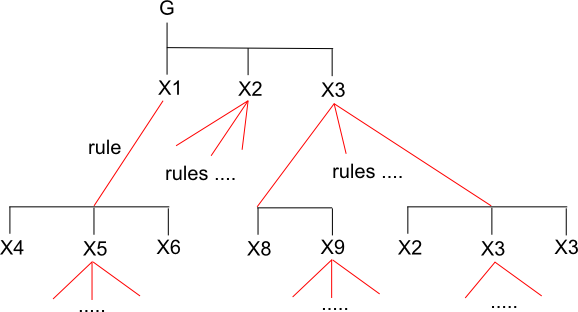
\includegraphics[scale=0.8]{and-or-graph.png}
% \caption{Plots of mean and variance; output vs input}
\end{figure}

\textbf{Complexity.}  If $m$ is the average number of rules applicable to a head predicate, $n$ is the average number of arguments for each rule, and $h$ is the depth of the search tree, then the size of the tree is $O((m \cdot n)^h)$.  Let me make a wild guess that $m \approx 30, n \approx 5, h \approx 5$, then size $\approx 10^{11}$.  This sounds manageable, but don't forget that the complexity of learning is the exponentiation of this!  So it is important to keep things simple at this stage.

\textbf{Efficient deduction.}\\
1.  Inference is often grounded by facts in \textbf{Working Memory} (ie, things that the AGI is currently paying attention to), though it may also be grounded by facts recalled from LTM (Long Term Memory).  Perhaps an efficient search algorithm should \textit{simultaneously} use backward chaining from the goal and forward chaining from ground facts under current attention.\\
2.  Given a head predicate, the KB server can quickly retrieve a list of all rules with that predicate by looking up an index.  Also, this list can be assumed to be sorted in order of confidence (remember that each rule is associated with a frequentist confidence).  This order may provide a basis for best-first / heuristic search\\
2.  Maybe the search should be randomized, and maybe it can start from the ``middle'' (ie, we generate an initial proof that is incorrect or incomplete, then repeatedly mutate it to make it correct)\footnote{This idea is inspired by the GSAT and WalkSAT algorithms for propositional logic.}.  This suggests using an evolutionary algorithm, but EA's may be slow. \{ TO-DO:  explore this idea further \}

Solving this search problem is very important because inductive learning also depends on such a search.

\section{Abduction}
\label{sec:abduction}

(Logic-based) abduction and induction are closely related;  they are 2 faces of the same coin.  In both cases we seek a hypothesis $H$ that together with background knowledge $B$, entails a positive example $e^+$:
$$ B \cup H \vdash e^+ $$
the only difference is that for abduction, $H$ is ground (ie, contains no variables); and for induction, $H$ is non-ground.

In classical logic, the algorithm for abduction is identical to deduction (backward chaining) except that the termination criterion is different.  In deduction the leaves of the search tree should be ground facts in the KB (which are believed to be true).  For abduction, the leaves should be so-called \textbf{abducibles}, which are propositions that can be assumed to be true.  For example, ``rain'' is a common occurrence and thus can be assumed to be true in order to account for the grass being wet.

Under probabilistic logic, we no longer need the notion of abducibles.  Interestingly, in this case the algorithm for abduction becomes almost identical to that of deduction, with the exception that deduction starts with an unknown fact whose truth is to be determined; whereas abduction starts with a known fact in need of explanations.  The 2 search spaces are exactly the same.

%Z abduction sometimes gives out-of-bounds Z values.\\
%\hspace*{1cm} $ z_1 \widetilde \vee z_2 = high $\\
%\hspace*{1cm} $ z_1 = low $\\
%\hspace*{1cm} $ \Rightarrow z_2 > 1.0 $
%
%Also, there are always 2 solutions, and they are within-bounds in the $z_1 > 0.5$ regime. Why?
%
%In fact, abduction using a rule with a point-Z-value is very unnatural.  Perhaps if we use $P(Z)$ the problem will be resolved?  But the ``2 roots'' problem seems to remain...

\chapter{Pattern recognition}
\label{ch:pattern-recognition}
\minitoc

The diagram below is due to David Marr:
\begin{figure}[H]
\centering
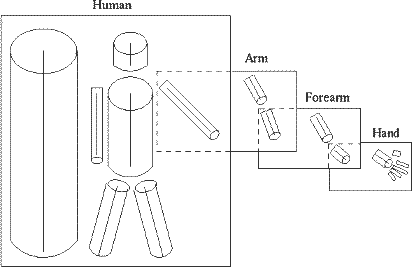
\includegraphics[scale=0.7, bb=0 0 414 269]{Marr3DModel.PNG}
\end{figure}

A highly simplified example of pattern recognition is the visual recognition of a human body by a Prolog rule such as\footnote{
Note that these concepts refer to \textit{visual features} rather than ideas  (The abstract concept of a human can be recognized via a larger set of rules that includes the visual rules).  The visual features should also be related to each other by some spatial predicates, but we ignore them here.  The details of visual recognition is explained in \S\ref{ch:vision}.
}:\\
\hspace*{1cm} \code{human :- head, torso, arm1, arm2, leg1, leg2.}\\
and each body part can be further recognized by its components such as:\\
\hspace*{1cm} \code{arm1 :- upper-arm, forearm, hand, fingers.}

In general the mechanism for pattern recognition is \textbf{forward-chaining} because we start with the premises (sensory input) and we do not know the desired conclusions in advance.

\section{The theory-based theory}

Concept formation (or ``categorization'' in the cognitive science literature, \citep*{Murphy2002}, \citep*{Cohen2005}, \citep*{Margolis1999}, \citep*{Lakoff1987}) is the task of using machine learning to learn common-sense concepts (\citep*{Nakamura1993}, \citep*{Wrobel1994}).  \citep*{Wrobel1994} has summarized the following properties of human concepts:
\begin{compactenum}[1.]
\item concepts often have non-necessary features
\item disjunctive concepts (there may not be any features that are shared by all members of a concept)
\item relational information (seems to require first-order logic to represent)
\item some features are themselves concepts
\item typicality (people can often rank examples according to typicality, eg the most typical fruit is orange)
\item basic levels (people are more adapt at categorization at certain basic levels, eg naming an object ``chair'' rather than ``office chair'' or ``a piece of furniture'')
\item superordinate distance (eg ``chicken'' is rated more similar to ``animal'' than to ``bird'')
\item unclear cases (eg ``is tomato a fruit?'')
\item context-dependent effects
\item goal-dependent effects
\end{compactenum}

There are two major theories of categorization:  In the \textbf{Classical view} a concept is defined by a set of defining features which are individually necessary and sufficient.  This view has very few adherents now.  The other major theory is the \textbf{Exemplar view}, which classifies instances based on their similarity (eg a distance metric) to a set of existing exemplars.

In my opinion, also shared by \citep*{Murphy1985} and \citep*{Wrobel1994}, the most satisfactory solution (aka the \textbf{theory-based theory}) is to view categorization as an \textit{inference} process, where concept formation means constructing \textit{explanations} of why certain objects belong to a concept.

\section{Similarity}
\label{sec:similarity}

Similarity is an essential component of commonsense reasoning.  For example, if we are told that "the whale is like a fish except that it is a mammal" we could draw the conclusion that the whale can swim (because fishes usually can swim) \footnote{But we would not conclude that the whale lays eggs because mammals don't lay eggs and we know that the whale \emph{is} a mammal, but it is only similar to a fish, and "is" is stronger than "similar to".}.
  
The similarity measure may also help in associative recall (\S\ref{sec:associative-memory}).

Similarity can be defined as an equivalent relation $\approx$, analogous to the equality relation $=$.  For example we can write\\
\tab $\mbox{whale} \approx \mbox{fish}$.

Recall that equality ($=$) is defined by \textbf{Leibniz's axiom of extensionality} -- which states that 2 entities are the same if every property of one is also a property of the other.  In type theory it can be stated as:
\begin{equation}
\forall x [f x = g x] \Rightarrow f = g
\label{eqn:Leibniz-extensionality}
\end{equation}
with $x : \beta$ and $f, g : \beta \rightarrow \alpha $.  This definition of $=$ is given by Church's type theory in 1940.  It defines equality for any function / predicate / proposition.

The similarity $\approx$ can be regarded as the probabilistic version of $=$.  We can simply replace the $\forall$ quantification in (\ref{eqn:Leibniz-extensionality}) with the probabilistic quantification $\#$ (\S\ref{sec:probabilistic-quantifier}), as in:
\begin{equation}
\# x [f x = g x] \Rightarrow f \approx g.
\label{eqn:probabilistic-extensionality}
\end{equation}
And because we can use fuzzy truth values, the $=$ on the LHS can also be replaced with a fuzzy version and we might denote it as $\approx$ as well:
\begin{equation}
\# x [f x \approx g x] \Rightarrow f \approx g.
\label{eqn:probabilistic-extensionality}
\end{equation}

But there is one problem.  In the whale $\approx$ fish example, the similarity is there not because the whale and fish predicates can apply to many common members (in fact, the 2 classes have no overlaps);  but because there are \textit{other} predicates that apply to both of them as objects.  For example:

\tab \tab \tab
\begin{tabular}{l|l}
has-fins(whale)        & has-fins(fish)\\
lives-in(whale, water) & lives-in(fish, water)\\
vertebrate(whale)      & vertebrate(fish)\\
\end{tabular}

How to capture this?  The solution is to ``turn around'' Leibnez's definition thusly:
\begin{eqnarray}
\mbox{(Leibnez)}           & \forall z. [x z = y z] \Rightarrow& x = y \\
\mbox{(inverted Leibnez)}  & \forall z. [z x = z y] \Rightarrow& x = y
\label{eqn:inverted-extensionality}
\end{eqnarray}
where I have renamed the variables to stress the symmetry.  And the probabilistic form is:
\begin{equation}
\# z [z x \approx z y]  \Rightarrow x \approx y.
\end{equation}
Notice that if we use higher-order logic, $z$ can be \textit{instantiated} as n-ary predicates with other arguments, eg
 $$z(x) = \mbox{lives-in}(x, \mbox{water})$$
so this is a very powerful way to express all possible forms of similarities.  This may be regarded as a logic-based, alternative formulation of Ulf Grenander's Pattern Theory \citep*{Grenander2007}.  One obvious complaint is that higher-order unification is highly intractable.  But this seems to be the correct formulation of the problem that we must use heuristics to deal with.

\{ To-do:  I need to develop the above theory further.  Milner's Context Lemma in domain theory (see eg \citep*{Streicher2006}) seems to have some semblance to what we're doing here.  Milner's Lemma states the equivalence of 2 orderings, $<_{\sigma}$ and $\sqsubset$.  They are defined by:
\begin{eqnarray}
M \sqsubset N  \quad  &\mbox{iff}& \quad \forall z \in \setN. \; M \Downarrow z \Rightarrow N \Downarrow z \\
M <_{\sigma} N \quad  &\mbox{iff}& \quad \forall Z \in \mbox{programs.} \; Z(M) \sqsubset Z(N)
\end{eqnarray}
where $M \Downarrow z$ means $M$ evaluates to $z$.  The situation kind of resembles Leibniz's definition and its inverted form.
\}

We'd be interested in measuring similarities between entities with certain structures.  This has been considered, eg in \citep*{Schmid2003}, chapters 10-12, in an ILP setting.  A famous example is the similarity between the solar system and the atom:  the important point is that both systems have bodies revolving around a central body, but it does not matter what their size, mass, and temperature, etc, are.

\{ The text that follows is outdated... \}
\underconst

What we seek is a correspondence between 2 structured entities, and to quantitatively measure the strength of such a correspondence.  Perhaps we can count the number of relations common to both entities.

\subsection{Motivating examples}

(A) ``Marmite is similar to Vegemite''\\
\hspace*{1cm} \begin{tabular}{l|l}
salty(marmite)                   & salty(vegemite)\\
dark-brown(marmite)              & dark-brown(vegemite)\\
yeast-extract(marmite)           & yeast-extract(vegemite)\\
rich-in(marmite, vitamin B)      & rich-in(vegemite, vitamin B)\\
sub-string(name(marmite),"mite") & sub-string(name(vegemite),"mite")\\
popular-in(england)              & popular-in(australia)
\end{tabular}

So I propose that the similarity between 2 objects can be calculated by considering all predicates that apply to both objects and obtaining the ratio between the number of identical and different predicates:
\begin{equation}
\mbox{similarity } \; \psi = \frac{N^{=}}{N^{=} + N^{\neq}}
\end{equation}

\{ TO-DO:  If the predicates have complex structure, we need to (recursively) compare the other arguments, and if the latter are different, adjust for their differences. \}

The above calculation can also be weighted by \textbf{information utility}, yielding the \textbf{subjective similarity} measure.

NOTE:  (B) is a bad example and should be replaced by something else.\\
(B) ``Lincoln is similar to Kennedy''
\footnote{In this example I have used my own knowledge representation scheme Geniform.  The example is based on a series of uncanny coincidences between the Lincoln and Kennedy assassinations that are often cited in trivia books.}
\\
\hspace*{1cm} \begin{tabular}{l|l}
elected-to-congress(lincoln, 1846)        & elected-to-congress(kennedy, 1946)\\
elected-president(lincoln, 1860)          & elected-president(kennedy, 1960)\\
succeeded-by(lincoln, vice-president$_1$) & succeeded-by(kennedy, vice-president$_2$)\\
\hspace*{1cm} name(vice-president$_1$, "johnson") &
\hspace*{1cm} name(vice-president$_2$, "johnson")\\
\hspace*{1cm} born(vice-president$_1$, 1808) &
\hspace*{1cm} born(vice-president$_2$, 1908)\\
assassinated$_1$(lincoln, friday)         & assassinated$_2$(kennedy, friday)\\
in(assassinated$_1$, theater)             & in(assassinated$_2$, car)\\
name(theater, "ford")                     & made(car, "ford")\\
with$_1$(wife(lincoln), lincoln)          & with$_2$(wife(kennedy), kennedy)\\
\hspace*{1cm} during(with$_1$, assassination$_1$) &
\hspace*{1cm} during(with$_2$, assassination$_2$)\\
\end{tabular}

Additionally:\\
\hspace*{1cm} name(car, "Lincoln")\\
\hspace*{1cm} has(kennedy, secretary), name(secretary, "Lincoln")

The additional facts do not increase the similarity, but they do make the 2 cases seem more ``connected''.

\underconst

(C) Some quantitative examples:\\
\hspace*{1cm} \begin{tabular}{|l|l|l|}
\hline
\textbf{the thing} & \textbf{approximated as} & \textbf{reason}\\
\hline
orange T-shirt     & red T-shirt      & proximity in color space\\
7 people           & several people   & $\catZ$\\
6'5 tall           & very tall        & $\catZ$\\
(John lies on several occasions) & John often lies & $\catP$\\
Stewart Shapiro    & Stuart Shapiro   & string edit distance\\
\hline
\end{tabular}

These examples can be represented and approximated by $\mathcal{P/Z}$ values (eg with fuzzy pattern recognition).

%orange(t-shirt) -> red(t-shirt)
%7*people -> several*people
%height(john,6.5) -> tall(john)
%(multiple facts) -> lies1(john), often(lies1)
%"Stewart Shapiro" -> "Stuart Shapiro"

(D) Some qualitative examples:\\
\hspace*{1cm} John is humorous $\approx$ John is witty\\
\hspace*{1cm} junk food, smoking and drinking $\approx$ unhealthy lifestyle\\
\hspace*{1cm} theft $\approx$ burglary\\
\hspace*{1cm} (complex scene) $\approx$ a fighting in a bar


\chapter{Belief revision}
\label{ch:belief-revision}

\minitoc

Belief revision concerns the problem of conflicting conclusions and, in the extreme, contradictions.

One simple question is:  If we arrive at two P(Z) distributions from two separate inference chains, how to combine the answers?

It seems that this is related to statistical inference.  Suppose we have a population.  A set of observations gives the estimate of the mean and variance:\\
\hspace*{1cm} $x_1, x_2, ..., x_{n_1} \sim Beta(\mu_1, v_1)$\\
Another set of observations gives another pair of estimates:\\
\hspace*{1cm} $y_1, y_2, ..., y_{n_2} \sim Beta(\mu_2, v_2)$\\
The question is to find a reasonable way to combine the 2 sets of observations to give a new estimate:\\
\hspace*{1cm} $x_1, x_2, ..., y_1, y_2, ... \sim Beta(\mu_0, v_0)$\\
In other words, how to express $(\mu_0, v_0)$ in terms of $(\mu_1, v_1)$ and $(\mu_2, v_2)$?

Maybe the $\mu_0$ is just the weighted average of $\mu_1$ and $\mu_2$?  $n_1, n_2$ can be assumed to be equal to the supports $w_1, w_2$ which can be calculated from the confidences $c_1, c_2$.

Some assumptions in the above may not be entirely justified:  the population size is typically small and the 2 samples may have overlap, ie, not independent.

\section{Justifications}

Justifications are the reasons why we believe in something.

\textbf{Justification-based Truth Maintenance Systems} (JTMS) keep track of justifications explicitly.  They are needed because otherwise we would not be able to recall why certain beliefs are in the mind.

\{ TO-DO:  For example... \}

This may be a requirement in addition to probabilistic reasoning.

\section{Many-worlds representation}

\begin{flushright}
\emph{The test of a first-rate intelligence is the ability\\
to hold two opposed ideas in the mind at the same time,\\
and still retain the ability to function.}\\
--- F Scott Fitzgerald
\end{flushright}

With probabilistic logic, it may be possible to represent multiple possible worlds in a single KB, by storing multiple potentially-conflicting assumptions in the KB.

For example, in the \textit{Truman Show} movie, there may be 2 competing assumptions in Truman's mind:\\
\hspace*{1cm} A1.  Truman's world is normal.\\
\hspace*{1cm} A2.  Turman's world is populated by fake actors.

In binary logic we can only accept either A1 or A2, thus the belief revision problem becomes unnecessarily much harder.

If we use probabilistic logic, then all we need is to impose that probabilities of alternative assumptions (ie, mutually exclusive or disjoint events) sum to 1.  Disjoint means that $P(A \cap B) = 0$, ie, A and B cannot be true at the same time.  The general rule is:\\
\hspace*{1cm} If we have a set of assumptions such that $P(A_i \cap A_j) = 0 \; \mbox{for all} \; i \neq j$,\\
\hspace*{1cm} then $\sum P(A_i) = 1$.

\subsection{Deliberative assumptions and ATMS}

Sometimes we make deliberative assumptions for more efficient reasoning, for example:  \textit{``Assuming the teacher will not check, I copy my classmate's homework''}.

This is in contrast to the kind of \textbf{implicit assumptions} described above, which are treated probabilistically, for example:  ``The teacher may check my homework with probability 0.2''.

The difference is that we deliberately force the reasoner to speculate on the consequences of an assumption as if its probability is 1.

This kind of reasoning is similar to binary logic, in which we must be careful about keeping track of conflicting assumptions.  \textbf{Assumption-based Truth Maintenance Systems} (ATMS) are developed specifically for this purpose.

ATMS seems somewhat redundant if we have probabilistic logic, where we can deal with multiple assumptions without probabilistic conflict (which in binary logic would result in conflicts).

If an assumption is particularly important, a probabilistic reasoner can take expected utilities into consideration.

\section{Consistency check}
\label{sec:consistency-check}

A few types of consistency checks are needed.

\section{Conflict resolution}
\label{sec:conflict-resolution}

Ie, what to do when an inconsistency is found.

\section{Theory revision}

See \S\ref{sec:inductive-learner}.


\chapter{Inductive learning}
\label{ch:machine-learning}
\begin{flushright}
\emph{Rewards and punishment is the lowest form of education.}\\
--- Zhuangzi (4th Century BC)
\end{flushright}
\minitoc

Note:  reinforcement learning is discussed in \S\ref{sec:RL}.

\section{``Learn by being told''}
\label{sec:learn-by-being-told}

This is probably the most efficient learning method.  (As Martin Magnusson pointed to me, \citep*{Perlis1996} explored the possibility where a human is able to teach an AI via natural-language conversations.  The paper contains hypothetical examples of some such conversations.)

\textbf{The Tell-Learn loop.}  Translate a natural language sentence into a logical formula.  Then the logical formula will directly enter the KB as knowledge, which is a very efficient way of learning.

The main difficulties in this loop are:
\begin{compactenum}[1.]
\item  The assimilation of the fact into the KB, which requires belief revision
\item  The translation from natural language to logic;  sometimes this require abductive reasoning even when the NL parser does an adequate job
\item  Surprisingly, inductive learning is also needed (see below)\\
\end{compactenum}

The base logic should be:\\
1. simple, for machine learning\\
2. close to NL, for easy translation from NL to logic.

\section{Background}
\label{sec:inductive-learner}

Inductive learning using logic is studied under the heading ILP (inductive logic programming; an excellent and up-to-date survey of which is \citep*{Konstantopoulos2008}).  The area known as theory revision is also essential to AGI (an excellent new book on ILP that discusses theory revision is \citep*{DeRaedt2008}).  Other notable books on induction / ILP are: \citep*{Holland1986}, \citep*{Muggleton1992}, \citep*{Lavrac1994}, \citep*{Bergadano1996}, \citep*{Nienhuys-Cheng1997}, \citep*{Flach2000}, \citep*{Lloyd2003}, \citep*{Getoor2007}, \citep*{DeRaedt2008}.

Induction is the dual of abduction:  both seeks a hypothesis $H$ to explain an example $e$:\\
\hspace*{1cm} $H \cup KB \vdash e$\\
\hspace*{1cm} abduction seeks an $H$ that is a ground fact\\
\hspace*{1cm} induction seeks an $H$ that is a general rule (ie, containing variables)

\textbf{Why is ILP needed?}  From my observations, when people use natural language to express ideas, they usually leave many \textbf{gaps} that must be filled by abductive or inductive reasoning.  A parser can translate NL sentences into logic \textit{literally}, but the resulting KB would be incapable of reasoning.

Filling in the logical gaps is very hard for humans because the inference of the gaps are inaccessible to conscious thinking.  Therefore, an inductive machine learner is required to perform this function.

\section{Examples}

\textbf{A. ``Women usually have long hair''}

Example facts:\\
\hspace*{1cm} Mary is a girl, Mary has long hair\\
\hspace*{1cm} Jane is a girl, Jane has long hair\\
\hspace*{1cm} John is a guy, John has short hair\\
\hspace*{1cm} etc...\\
To learn:\\
\hspace*{1cm} female(X) $\rightarrow$ long-hair(X)\\

This example illustrates the \textbf{MDL principle}:  The general rule \textit{covers} many examples and thus is \textit{compressive} -- In some situations, we may forget individually which woman has long hair, while remembering a group of women as mostly having long hair (eg, after seeing a group of choir singers).

We can make this example more complex by adding the role of a speaker:\\
\hspace*{1cm} The teacher tells me ``Mary has long hair''\\
\hspace*{1cm} The teacher tells me ``Mary is a girl''\\
\hspace*{1cm} The teacher tells me ``Jane has long hair''\\
\hspace*{1cm} The teacher tells me ``Jane is a girl''\\
\hspace*{1cm} etc...

We can have the general rule:
\footnote{In this example we have used 3 tricks:\\
a. propositions as variables\\
b. quoted formulae\\
c. equality\\
just for the sake of illustration.  The actual KR scheme is still undecided.}\\
\hspace*{1cm} \textit{``If a speaker is a credible source, then what s/he says can be assumed to be true''}\\
\hspace*{1cm} \textbf{R1:} \quad credible(X) $\wedge$ says(X,Y) $\rightarrow$ Y

But notice that R1 can cover the girls examples only if we include the quoted sentences:\\
\hspace*{1cm} \begin{tabular}{l l}
R1 $\wedge$ Y=long-hair(mary) & $\vdash$ long-hair(mary)\\
R1 $\wedge$ Y=female(mary)    & $\vdash$ female(mary)\\
R1 $\wedge$ Y=long-hair(jane) & $\vdash$ long-hair(jane)\\
R1 $\wedge$ Y=female(jane)    & $\vdash$ female(jane)
\end{tabular}

Thus, we can further compress the right hand sides with this rule:\\
\hspace*{1cm} \textbf{R2:} \quad female(X) $\rightarrow$ long-hair(X)\\
or compress what the teacher says:\\
\hspace*{1cm} says(teacher,"female(X) $\rightarrow$ long-hair(X)")

This shows that even when an example is explained (entailed) by a general rule (R1), it may still require compression (R2).  This is different from the traditional ILP goal which is simply to ``cover'' (ie entail) positive examples.  Now we need to find \textit{all possible} ways to compress the KB.

\textbf{B. Roman numerals}

Example facts:\\
\hspace*{1cm} Roman numeral 1 is \code{I}\\
\hspace*{1cm} Roman numeral 2 is \code{II}\\
\hspace*{1cm} Roman numeral 3 is \code{III}\\
To learn:\\
\hspace*{1cm} Roman numeral $n$ is $n$ \code{I}\\
(which is wrong, but is reasonable in common sense).

\section{Complexity}

\subsection{Inducing one hypothesis}

The main task of ILP is to search in the hypothesis space $\Hyp$ specified partly by the logical syntax (such as $\catPZ$ logic) and partly by background knowledge (eg what kind of predicates are present).  The hypothesis space is structured into a lattice with a partial order (usually denoted $ \preceq $).  The partial order can be one of \textbf{$\theta$-subsumption}, LGG (\textbf{least general generalization}), or \textbf{logical entailment}.  These have subtle differences, with logical entailment being the most rigorous.  The searcher can traverse up and down the lattice, corresponding to \textbf{generalization} and \textbf{specialization} of the hypothesis.  These 2 are known as \textbf{refinement operators}.  Because there are so many ways to generate hypotheses in FOL (with many predicates to choose from, and the possibility of introducing variables as desired), the branching factor is extraordinarily high.  Also, the lattice can be infinite, so we need to limit its depth.

Another problem is that, once a hypothesis has been generated, it must be tested against the rest of the KB for \textbf{consistency}.  The consistency check must also be limited in depth, but even then it is very time-consuming.

Much of the complexity of induction occurs in the ``inventive step'', whereby a new rule is generated.  The inventive step can draw upon knowledge from the entire KB, which makes it combinatorially explosive.  Currently the most promising idea I have is to ``recall similar examples'' -- that means, we perform an \textbf{associative memory search} to recall examples similar to the current experience, and only then do we try to generalize from the experience plus the recalled examples.  But this strategy merely pushed the responsibility to the associative memory to recall only the most \textbf{salient / relevant / interesting} examples.  Still, this trick seems to be more efficient than blind search.

Another promising idea is that some of the more intensive processing can be performed during \textbf{sleep}.

\subsection{Inducing a whole theory}
\label{sec:complexity-of-hypothesis-space}

Let $\Hyp$  denote the hypothesis space (ie, space of all logic formulae).  The size of $\Hyp$ is huge (see above).\\
A logical theory $T$ is a set of hypotheses, $ \{ h_i | h_i \in \Hyp \} $.  Note that $ T \in 2^{\Hyp} \;$ which is a hugely huge space.\\
Let $E$ denote the set of examples $\{ e_1, ... \}$ that should be covered by the target theory.\\
So we're seeking an optimal theory $T^*$ such that it covers all examples and is succinct, ie:\\
\hspace*{1cm} $ T^* \vdash \{ e_i \} $ \quad and \quad $ |T^*| $ is minimal.

There is hope, since we can \textit{seed} the initial theory with human knowledge.  In other words, we can start with a $T_0$ which contains a large number of logic statements translated from NL.

Even if we do that, we can realistically only store one theory in memory.  When we evaluate a new hypothesis $h$ to cover an example $e$, ie, to test whether\\
\hspace*{1cm} $h \cup T \vdash e \; ?$\\
we have to bear in mind that we are just testing the hypothesis $h$ w.r.t. \textit{one} background theory.  This means that $h$ may have a different score when $T$ changes;  but unfortunately we cannot realistically keep track of different scores of $h$ against different theories.  In other words, the scores we keep will be somewhat \textit{inaccurate} and are \textit{relative} to a constantly changing candidate theory.  \{ TO-DO:  Due to the use of probabilistic logic, we can store multiple sets of hypotheses simultaneously.  Revise this paragraph. \}

\section{Compression}
\label{sec:compression}

In general, compression is achieved via \textbf{pattern recognition} (\S\ref{ch:pattern-recognition}).  Upon the arrival of new sensory input, the Pattern Recognizer is invoked to recognize patterns in the data (the process is forward-chaining).  Due to the use of \textbf{fuzzy} pattern recognition, the result may be lossy, which is good.

\textbf{Decompression} is a special form of abduction:  starting from the recognized patterns (facts) we try to abduce the original low-level sensory facts.  (Though we're usually not interested in low-level facts during normal abduction.)

Inductive learning is a kind of dual of pattern recognition:  whereas pattern recognition recognizes patterns using some logic rules, inductive learning learns those rules.  The job of the Inductive Learner is to generalize from regularities in the sensory input whenever possible, adding new rules to the KB.

In summary:\\
\hspace*{1cm} compression = pattern recognition = forward chaining\\
\hspace*{1cm} decompression = abduction = backward chaining\\
\hspace*{1cm} learning to compress = backward chaining with rule invention

\textbf{Formal definition.}  The goal is to find a theory $T$ to compress a set of examples $E = \{ e_i \}$ such that:\\
\begin{equation}
\left
\{
\begin{array}{c@{\quad\quad}l}
T \vdash \hat{E}  & \mbox{(reconstruction of memory)}\\
\hat{E} \approx E & \mbox{(approximation)}\\
|T| \leq |E|      & \mbox{(smaller description length)}
\end{array}
\right.
\end{equation}
Note:  the entailment $\vdash$ should be fuzzy/probabilistic.

\textbf{About coverage.}  Usually, an example can be covered (entailed) by a number of alternative proofs.  This is probably very common.  For example:\\
\hspace*{0.8cm} \begin{tabular}{l l}
Mary doesn't love John & $\vdash$ John is unhappy\\
John doesn't love Kate & $\vdash$ Kate is unhappy\\
Pete has no money      & $\vdash$ Pete is unhappy
\end{tabular} \vspace{-0.2cm}

but we can further compress the right hand sides by:\\
\hspace*{1cm} everyone is unhappy\\
even though the right hand sides were entailed by 3 different reasons.

Having a large number of general rules enables better \textbf{reconstruction} of past memories.  Better reconstruction is clearly an advantage from a utilitarian perspective as we often do not know in advance what memories may be useful later.  (Overlapping coverage may be a by-product of having a large number of rules.)

We can define \textbf{information utility} as the utility of information items ($U: \{ \mbox{infon} \} \rightarrow \setR$)
\footnote{An infon is informally defined as a discrete information item.  In practice it can be any proposition in the KB.}
, as a generalization of utility over states ($U: \{ \mbox{state} \} \rightarrow \setR$).  Then the goal of compression is to \textit{minimize reconstruction errors (weighted by information utility) with the smallest theory}.  This is in keeping with the MDL principle.

%Note:  $T$ may contain ground facts that are absent in $E$.  For example, we may remember that many women in the choir have long hair (a ground fact in $T$) but we may not remember exactly who has long hair (ground facts in $E$).

%The error $D = \mbox{Diff} (\hat{E}, E)$ is in general very difficult to calculate, as it involves the differences between things like:\\
%\hspace*{1cm} blonde $\approx$ brunette\\
%\hspace*{1cm} chair $\approx$ desk\\
%\hspace*{1cm} humorous $\approx$ witty\\
%which seems to involve a similarity measure (\S\ref{sec:similarity}).  But we can focus on the subclass of \textbf{compressive approximations} where Diff() can be defined more easily.

In traditional ILP with binary logic, we settle at finding a theory that covers all positive examples and none of the negative examples.  In the compression setting, mere coverage is not enough:  we should generate new rules even when the data are already entailed by some existing rules, because the new rules can further compress data.

%A possible scoring function is:\\
%\hspace*{1cm} $S = -kD - |T|$\\
%where $k$ is some constant.
%
%A brute-force algorithm is to search all possible sets of hypotheses ($2^{\mathbb{H}}$) and output the one with the best score, which is obviously impractical.  A local search algorithm may start with a seed theory and try to search in its neighborhood.  For this purpose we need an \textit{incremental} scoring function:\\
%\hspace*{1cm} $\Delta S = -k \Delta D - \Delta |T|$
%
%\begin{algorithm}[H]
%\caption{Naive compressor}
%\alginout{examples $E$}
%{a theory $T$}
%\begin{algtab}
%\alglabel{alg:naive-compressor}
%
%start with a seed theory\\
%
%\algrepeatforever
%	get examples from sensory experience\\
%
%	(randomly/heuristically) add/subtract/modify facts/hypotheses in $T$\\
%
%	if $\Delta S > 0$ accept the changes\\
%\algend
%
%\end{algtab}
%\end{algorithm}
%\vspace{-0.7cm}
%
%The calculation of $\Delta S$ may be time consuming as it involves reconstructing $\Delta\hat{E}$ and then finding the error $\Delta D$.

\subsection{Plateau phenomenon (local minima)}

Some changes in $T$ may increase the error first but further changes in that direction may result in a smaller error.  This phenomenon (ie, local minima) is common in ILP and makes learning more difficult.

An example is given in \citep*{Bergadano1996}, p89, for the learning of the Prolog function \code{append/3}.  The positive and negative examples are:\\
\hspace*{1cm} \begin{tabular}{l l}
$e^+$: & \code{append([0],[1,2],[0,1,2])}\\
       & \code{append([],[1,2],[1,2])}\\
$e^-$: & \code{append([0],[1,2],[0,1])}\\
       & \code{append([0],[1,2],[1,2])}\\
       & \code{append(0,1,[0,1])}\\
       & \code{append(a,b,[a,b])}
\end{tabular}

And the target clause is:\\
\hspace*{1cm} \code{append(X,Y,Z) :- list(X), head(X,X1), tail(X,X2), append(X2,Y,W), cons(X1,W,Z)}

The learning of the first literal, \code{list(X)}, would indeed have positive information gain
\footnote{The definition of information gain is that used by the ILP program FOIL.  See the book for details.}
 as it excludes the last 2 negative examples;  but the addition of the following 3 literals would have small or even negative information gain, until the last literal is reached and all positive and negative examples are covered.

\subsection{Minimum description length}

An interesting observation (noted in \citep*{MacKay2003} Chapter 28, and \citep*{Chater2005}) is the equivalence of MDL and Bayesian likelihood maximization:  Given the data $D$, The goal of perception is to choose the hypothesis $H^*$ that maximizes $P(H|D)$.  According to Bayes theorem, this is equivalent to choosing the $H^*$ that maximizes $P(D|H)P(H)$, where $P(H)$ represents some sort of subjective prior bias.  The $H^*$ that maximizes $P(D|H)$ is the same $H^*$ that minimizes the negative of the logarithm of this term, which can be written:\\
\hspace*{1cm} $-\log_2 P(H) - \log_2 P(D|H)$.\\
By Shannon's coding theorem, the optimal code length for a probability $p$ is $-\log_2 p$, so we can interpret the above as:\\
\hspace*{1cm} codelength($H$) + codelength($D|H$).

Note:  the MDL terminology is different from the logic terminology:\\
\hspace*{1cm} \begin{tabular}{l l l}
\textbf{in MDL}       & \textbf{in logic}\\
\hline
a hypothesis          & is called a logical theory\\
N/A                   & a hypothesis (= part of a logical theory)
\end{tabular}

\{ TO-DO:  How does this shed light on the logical compression algorithm? \}

%\section{Evolutionary algorithms}
%
%It seems that EA, as a global optimization technique, can be a good choice for the ILP search.  There are two general approaches to GA (\citep*{Freitas2002}):
%
%In the \textbf{Pittsburgh approach}, each individual in the EA population represents \textit{a set of rules}, ie, an entire candidate solution.
%
%In the \textbf{Michigan approach}, which departs from conventional EA's, each individual represents \textit{a single rule}, ie, a part of a candidate solution.
%
%It seems to me that we need the Michigan approach.
%
%TO-DO:  how to learn hybrid logical rules.
%Learning of Z rules is based on examples with explicit Z values;\\
%Learning of P rules is based on examples that are true or false.\\
%So they may be learned independently?
%
%Besides Michigan vs Pittsburgh, one more thing is the role of a lot of background knowledge.  How might this change things?

\section{Algorithm}

(Cf algo~\ref{alg:top-level-sensory-processing} for the top-level algorithm of the logical reasoner.)

The goal of the learning algorithm is to produce useful generalizations, or we can say the most \textit{compressive} generalizations.

\underconst
\hrule

\begin{algorithm}[H]
\caption{Practical inductive learner}
\alginout{incoming facts}
{1 or more hypotheses}
\begin{algtab}
\alglabel{alg:practical-inductive-learner}

Try to recall similar examples from memory.\\

Invent a hypothesis to generalize the new fact + examples\\

\end{algtab}
\end{algorithm}
\vspace{-0.7cm}

I look at the problem from a perspective that is slightly different from the one prevalent in the ILP literature.  Most ILP methods search in the \textit{hypothesis space}, but I find it easier to think about the problem in \textit{proof space}:\\

\begin{compactenum}[\textbullet ]
\item  My algorithm searches for explanations of \textit{one incoming fact} while inventing (possibly many) hypotheses along the way.

\item  The hypothesis-space algorithm, on the other hand, focuses on \textit{one hypothesis}.  It would pick some examples (past or incoming facts) and move around the hypothesis lattice in order to cover them, ie, keeping a score of the numbers of positive and negative examples that are covered or not.  And it seeks the hypothesis with the best score.\\
\end{compactenum}

%A problem with hypothesis-space search is that all the examples relevant to a hypothesis do not come at the same time.  In real experience, the examples are usually scattered over a long time span.

%\{ TO-DO: how to combine the 2? \}


\chapter{Natural language}
\label{ch:natural-language}
\begin{flushright}
\emph{The fish trap exists because of the fish; once you've gotten the fish,\\
you can forget the trap. The rabbit snare exists because of the rabbit;\\
once you've gotten the rabbit, you can forget the snare.\\
Language exists because of meaning; once you've gotten the meaning,\\
you can forget language.}\\ --- Zhuangzi (4th Century BC)
\end{flushright}
\minitoc

\section{Natural language is not essential to AGI}

Our approach is to define a logic that can faithfully render arbitrary natural-language texts.  We call such a logical form Geniform.  The translation of NL to Geniform can itself be encoded as logical rules, thus the parsing of NL can be achieved via logical inference (as forward-chaining in a bottom-up manner).  And since logical inference is reversible, the generation of NL will also come as free.

All the irregularities of NL will be taken care of via machine learning.

\subsection{Background: unification-based grammars}

The family of unification-based grammars includes LFG (Lexical Functional Grammar), HPSG (Head-Driven Phrase Structure Grammar), and PATR grammar.  The unification algorithm used in unification-based grammar is the same as the unification algorithm used in logic.  This is further evidence that the brain employs abstract symbolic processing similar to formal logic.

\subsection{Background: cognitive linguistics}

Our approach is closer to ``formal semantics''.  Many authors, most famously Richard Montague, have argued that natural languages are formal languages.  Some have also advocated the use of natural language as knowledge representation in AI.  Thus the line between formal and natural languages is blurred.

\todo{How may cognitive linguistics affect natural language processing in Genifer?}

\section{Abduction as interpretation}
\label{sec:abduction-as-interpretation}

\subsection{A detailed example}

The general sequence is:\\
\hspace*{1cm} tokenization $\rightarrow$ POS-tagging $\rightarrow$ syntax parsing $\rightarrow$ semantic parsing\\
which should be familiar to everyone with experience in NL processing.

I will explain the details using a simple example:\\
\hspace*{1cm} ``I love Mary''

The crucial thing is that we represent everything in a logic-based framework. First we represent the sentence as "raw data" (ignoring tenses to simplify matters):\\
\hspace*{1cm} $\mbox{sentence}(e_0)$\\
\hspace*{1cm} $\mbox{lexeme-I}(e_1)$\\
\hspace*{1cm} $\mbox{lexeme-love}(e_2)$\\
\hspace*{1cm} $\mbox{lexeme-Mary}(e_3)$\\
\hspace*{1cm} $\mbox{begins-with}(e_0, e_1)$\\
\hspace*{1cm} $\mbox{follows}(e_2, e_1)$\\
\hspace*{1cm} $\mbox{follows}(e_3, e_2)$\\
where:\\
\hspace*{1cm} the $e_i$'s are \textbf{entities} (logical constants).\\
\hspace*{1cm} the entities $e_1$, $e_2$, and $e_3$ are words.\\
\hspace*{1cm} follows() means a word follows another word in a sentence.

Up to now, all we have is a sentence as raw text (without meanings).  The next step is to recognize parts of speech (nouns, verbs, adjectives, etc). We can use logical rules to do this.

An example logical rule is:\\
\hspace*{1cm} $\mbox{lexeme-Mary}(X) \rightarrow \exists e \; \mbox{parse-as}(e, X) \wedge \mbox{noun}(e)$\\
which simply means that the word "Mary" is a noun. X is a variable (implicitly universally quantified). $e$ is a new entity, which instantiates to $e_4$ when the rule is applied.

We can also use logical rules to parse syntax. We can perform ``VP $\leftarrow verb + noun$'' with this rule\footnote{We need this special rule:\\
\hspace*{1cm} $\mbox{follows}(X_1, X_2) \wedge \mbox{parse-as}(X_1, X_3) \wedge \mbox{parse-as}(X_2, X_4) \rightarrow \mbox{follows2}(X_3, X_4)$ }:\\
\hspace*{1cm} $\mbox{verb}(X_1) \wedge \mbox{noun}(X_2) \wedge \mbox{follows2}(X_2, X_1) \rightarrow \exists e \; \mbox{parse-as}(e, X_1, X_2) \wedge vp(e)$\\
which creates a new entity $e_5$ which is a VP.

Assume that eventually we have a parse of the sentence S, $e_6$. Notice that up to now, it's all syntax parsing.

Next we perform semantic parsing.  The key is to generate partial meanings for phrases, such as the verb phrase ``loves Mary''.

\textbf{Lambda operator.}  In formal semantics, it is customary to use the $\lambda$ operator to represent the meaning of phrases.  The reason is that first-order logic do not have the expressive power to represent such phrases.  For example, the VP ``loves Mary'' denotes ``somebody's loving Mary'', which may be represented as $love(\_ \,,mary)$; but that is not a well-formed formula in FOL.  Instead we can represent it using the $\lambda$ expression $\lambda x \; love(x,mary)$.

\textbf{Composition of concepts.}  (For details see \S\ref{sec:composition})  Under this method, all phrases are represented by compositions.  For example, the VP ``loves Mary'' can be represented by $app(loves,mary)$, or in short form $mary \circ loves$.  This composite is a \textit{first-order object}, ie, a first-class citizen in the logic which can be further manipulated or modified, eg, when we compose it with $john$, we get $((mary \circ loves) \circ john)$ which is equivalent to the FOL statement $loves(john,mary)$.

I think this method is superior to $\lambda$ because the meanings of phrases can be represented by first-order objects.  It also makes semantic parsing very intuitive.

% \todo{Revise this example with the newly improved Geniform.}

\todo{Explain semantic parsing with examples.}

%A semantic rule is similar to a syntactic one:\\
%\hspace*{1cm} $\mbox{lexeme-love}(X) rightarrow \exists e \; \mbox{parse-as}(e, X) \wedge \mbox{verb}(e) \wedge \mbox{means}(e, \mbox{concept-love})$\\
%
%\hspace*{1cm} $\mbox{verb}(X_1) \wedge \mbox{np}(X_2) \wedge \mbox{follows2}(X_2, X_1) \wedge \mbox{means}(X_1, Y_1) \wedge \mbox{means}(X_2, Y_2)$\\
%\hspace*{1cm} $rightarrow \exists e \; \mbox{parse-as}(e, X_1, X_2) \wedge vp(e) \wedge \mbox{means}(e, comp(Y_1,Y_2))$\\
%
%For example, we can augment the syntactic rule\\
%\hspace*{1cm} $\mbox{VP} \leftarrow \mbox{verb}, \mbox{NP} $\\
%with\\
%\hspace*{1cm} $\mbox{VP}(\mbox{comp}(Sem_1,Sem_2)) \leftarrow \mbox{verb}(Sem_1), \mbox{NP}(Sem_2)$\\
%where the $Sem$'s are variables containing the ``semantics'' of phrases.\\
%\hspace*{1cm} $\mbox{S} \leftarrow \mbox{NP}, \mbox{VP} $\\
%\hspace*{1cm} $\mbox{S}(Predicate) \leftarrow \mbox{NP}(Subject), \mbox{VP}(Subject * Predicate) $\\
%\hspace*{1cm} $\mbox{VP}(X) rightarrow \mbox{com}(\mbox{loves},\mbox{mary})$\\
%which creates a new entity $e_7$ with the meaning of "love".\\
%\hspace*{1cm} $\mbox{lexeme-love}(X_1) rightarrow \exists e \; \mbox{concept}(e) \wedge \mbox{means}(e, \mbox{concept-love})$\\
%
%The final step of semantic parsing uses a special trick,  ``de-reification'' (\S\ref{sec:reification}):\\
%\hspace*{1cm} (assume that $e_{8}, e_{9}$ denote the persons John and Mary)\\
%\hspace*{1cm} $\mbox{de-reify}(\mbox{concept-love}, e_{8}, e_{9})$\\
%which generates the logical statement:\\
%\hspace*{1cm} $\mbox{loves}_1(e_{8},e_{9})$\\
%
%Finally we have:\\
%\hspace*{1cm} $\mbox{means}(e_0, \mbox{loves}_1)$

\section{Comprehensive grammatical categories of English}

Here are some NL grammatical categories (intended to cover as broadly as possible) and typical examples in English.  Designers of NL interfaces can supply translations to these examples.  [The contents in this section and all the examples are taken directly from the book "English Grammar" by Peter Collins, 1998, Addison Wesley.  \todo{NOTE:  This may be a copyright infringement but I have contacted the author without getting his reply.}]  This page is intended to provide a simple comparison of NL interfaces, not meant to be a standard grammar for AGI purposes.

\titleformat{\subsection}[hang]{\sffamily\bfseries\large\color{blue}}{(\Alph{subsection}) \hspace{5pt}}{0pt}{}

\setcounter{subsubsection}{1}
\renewcommand{\subsubsection}[1]{\sffamily{\bfseries{\color{blue}{ \stepcounter{subsubsection} (\Alph{subsection}.\arabic{subsubsection}) \hspace{5pt}#1}}}}

\newcounter{subsubsubsection}[subsubsection]
\newcommand{\subsubsubsection}[1]{\stepcounter{subsubsubsection} \sffamily{\bfseries{\color{blue}{ (\Alph{subsection}.\arabic{subsubsection}.\arabic{subsubsubsection}) \hspace{5pt}#1}}}}

\subsection{Nouns}

\subsubsection{Common nouns}

eg \english{chair}, \english{chairs}

eg \english{importance}

\subsubsection{Proper nouns}

eg \english{Australia}

eg \english{The Isle of Man}

\subsubsection{Pronouns}

eg \english{he}

eg \english{\textbf{our} chair} (possessive, as determiner)

eg \english{theirs}

eg \english{each other}, \english{one another} (reciprocal pronouns)

eg \english{this}, \english{that} (demonstrative pronouns)

eg \english{who}, \english{whom}, \english{whatever} (interrogative and relative pronouns)

eg \english{some}, \english{both}, \english{any}, \english{each}, \english{none}, \english{nobody} (indefinite pronouns)

\subsection{Verbs}

\subsubsection{Main verbs}

eg \english{kick}, \english{grow}

eg \english{to kick}, \english{kicked}, \english{kicking}, \english{kicks} (tenses and other inflections)

\subsubsection{Auxiliary verbs}

eg \english{can}, \english{have}, \english{haven't}

eg \english{She \textbf{is} dancing the lambada.}

eg \english{He \textbf{has} driven for 4 hours.}

\subsubsection{Operators}

eg \english{they \textbf{will} try their best}, \english{Sam \textbf{won't} play chess}

\subsection{Adjectives}

\subsubsection{Attributive (modifies a head noun)}

eg \english{the \textbf{loud} bell}

\subsubsection{Predicative}

eg \english{the bell was \textbf{loud}}

\subsubsection{Gradation}

eg \english{\textbf{very} loud}, \english{\textbf{a bit} loud}

\subsubsection{Comparison}

eg \english{louder}, \english{loudest}

\subsection{Adverbs}

eg \english{The policeman acted \textbf{decisively}}

eg \english{He is a \textbf{somewhat} shy young man}

eg \english{\textbf{Actually}, many of the lifeboats have been removed}

eg \english{Patrick has lost 2 games, \textbf{however} he could still win}

eg \english{more surprisingly}, \english{most surprisingly}

\subsection{Determinatives}

\subsubsection{Articles}

eg \english{the}, \english{a}, \english{an}

\subsubsection{Demonstratives}

eg \english{this}, \english{that}, \english{those}

\subsubsection{Interrogatives}

eg \english{which}, \english{what}

\subsubsection{Cardinal numerals}

eg \english{one}, \english{two}

\subsubsection{Quantifiers}

eg \english{both}, \english{all}, \english{every}, \english{any}, \english{no}, \english{much}, \english{less}

\subsubsection{Prepositions}

\subsubsubsection{Time}


eg \english{\textbf{after} our match}, \english{\textbf{during} the exam}

\subsubsubsection{Place}


eg \english{\textbf{in} the kitchen}, \english{\textbf{against} the wall}

\subsubsubsection{Manner}


eg \english{\textbf{with} ease}

\subsubsubsection{Agency}


eg \english{\textbf{by} the mechanic}

\subsubsubsection{Recipience}


eg \english{\textbf{to} a friend}

\subsubsection{Subordinates}

\subsubsubsection{Time}


eg \english{\textbf{until} it rains}, \english{\textbf{as} she spoke}

\subsubsubsection{Condition}


eg \english{\textbf{if} we win Lotto}, \english{\textbf{unless} a catastrophe occurs}

\subsubsubsection{Concession}


eg \english{\textbf{although} she likes coffee}, \english{\textbf{while} it was undoubtedly entertaining}

\subsubsubsection{Contrast}


eg \english{\textbf{whereas} Japan is a creditor nation}

\subsubsubsection{Exception}


eg \english{\textbf{except} he didn't have the strength}

\subsubsubsection{Reason}


eg \english{\textbf{because} the bus broke down}

\subsubsubsection{Comparison}


eg \english{you ate more peanuts \textbf{than} I did}

\subsubsection{Coordinators}

eg \english{Peter went to Paris \textbf{but} his family stayed home}

eg \english{Barbie was wearing a new bracelet \textbf{and} a diamond ring}

eg \english{Should we come before \textbf{or} after lunch?}

eg \english{\textbf{Both} Bill \textbf{and} his wife deny the allegations}

eg \english{She \textbf{neither} hates him \textbf{nor} loves him}

eg \english{It's \textbf{not} for you \textbf{but} for me}

\subsection{Phrases}

\subsubsection{Noun phrase (NP)}

eg \english{large birds with sharp claws}

eg \english{writers of science fiction, who are here for a conference}

\subsubsection{Verb phrase (VP)}

eg \english{[Lisa] \textbf{trains} 3 times a week}

eg \english{There I \textbf{am}, minding my own business, when this tall blonde \textbf{walks} up and \textbf{asks} me for a cigarette}

eg \english{Ken said, 'I \textbf{have} enough money' }

eg \english{[If I] \textbf{could} have my life over again, [I] \textbf{would} not change anything}

eg \english{[They should] \textbf{have reached} the peak by now}

eg \english{[Ken] \textbf{is} building a new house}

eg \english{[Many footballers] \textbf{get} injured}

\subsubsection{Adjective phrase (AdjP)}

eg \english{too rebellious}, \english{quite surprisingly intelligent}, \english{very slow}

eg \english{slower than a wet week}, \english{large for a goldfish}

eg \english{fiercer than I expected}

eg \english{sorry that he hurt her feelings} (noun clause)

eg \english{aware of the consequences} (of-PP)

\subsubsection{Adverb phrase (AdvP)}

eg \english{very quickly}, \english{most reluctantly}

eg \english{more defiantly than they had predicted}

\subsubsection{Prepositional phrase (PP)}

eg \english{\textbf{in} the water}

eg \english{\textbf{with} a spoon}

eg \english{[way] \textbf{below} standard}, \english{[just] \textbf{before} the start}

eg \english{Scott arrived \textit{in} \textbf{a limousine} \textit{with} \textbf{his girlfriend}}

\subsubsection{Genitive phrase (GP)}

eg \english{\textit{The princess's} popularity was greater than \textit{her husband's}}

\subsection{Clauses}

\subsubsection{Object vs predicative complements}

eg \english{Mary contacted \textbf{a police officer}} (object)

eg \english{Mary was \textbf{a police officer}} (predicative, \english{was}=copula)

\subsubsection{Subjective and objective predicatives}

eg \english{Indira was \textbf{generous}} (subjective)

eg \english{We considered Indira \textbf{generous}} (objective)

\subsubsection{Patterns of complementation}

\subsubsubsection{intransive (S P)}

eg \english{Sue \textbf{stumbled}}

\subsubsubsection{monotransitive (S P Od)}

eg \english{Sue \textbf{sipped a martini}}

\subsubsubsection{Copulative (S P PCs)}

eg \english{Sue \textbf{seems drunk}}

\subsubsubsection{Ditransitive (S P Oi Od)}

eg \english{Sue \textbf{offered her guests a martini}}

\subsubsubsection{Complex-transitive (S P Od PCo)}

eg \english{Sue \textbf{made them drunk}}

\subsubsection{Other complements}

\subsubsubsection{PP-complements of prepositional verbs}

eg \english{They have decided \textbf{on a short vacation}}

eg \english{He approves entirely \textbf{of your decision}}

eg \english{Geoff protected his little brother \textbf{from the bullies}}

eg \english{She blames all their problems \textbf{on his incompetence}}

\subsubsubsection{Adverbs as complement of phrasal verbs}

eg \english{Vera cried \textbf{out}}

eg \english{We give \textbf{up}}

eg \english{The umpires have called \textbf{off} the match}

eg \english{Please take the garbage \textbf{out}}

eg \english{We have come \textbf{up} \textbf{with an alternative plan}}

\subsubsubsection{Non-finite complements of 'catenative' verbs}

eg \english{I \textbf{plan} to \textbf{keep} applying for jobs}

eg \english{You should \textbf{stop} \textbf{trying} to \textbf{get} invited}

\subsubsection{Adjuncts}

AdvP: eg \english{very carefully}, \english{sometimes}, \english{moreover}

PP: eg \english{over the road}, \english{with a torch}

Subordinate clause:  eg \english{because it is raining}, \english{after the music stopped}

NP: eg \english{next Easter}, \english{this Friday}

types:

Time:  eg \english{at Easter}, \english{in 2 week's time}

Frequency:  eg \english{each Friday}, \english{on the hour}

Place: eg \english{in Bandung}, \english{on the summit}

Purpose: eg \english{in order to test the hypothesis}, \english{for a break}

Reason: eg \english{because he is shy}, \english{on the grounds of sanity}

Condition: eg \english{if you agree}, \english{unless it is convenient}

Manner: eg \english{more politely}, \english{with a spade}

Degree: eg \english{in my opinion}, \english{to be fair}, \english{unfortunately}

Connective: eg \english{consequently}, \english{in other words}, \english{however}

\subsubsection{Mood}

\subsubsubsection{Declarative mood}

eg \english{He is serious}

\subsubsubsection{Interrogative mood}

eg \english{Is he serious?}

eg \english{Anastasia has sent another e-mail, hasn't she?}

eg \english{Whose T-shirt is that?}

eg \english{Who can help me?}

eg \english{Where are my keys?}

\subsubsubsection{Imperative mood}

eg \english{Be serious}

eg \english{Give me some more money}

eg \english{Don't forget to write}

eg \english{Let's apply for a loan}

\subsubsubsection{Exclamative mood}

eg \english{How serious he is!}

eg \english{How many times have I asked you!}

\subsubsection{Negation}

clausal negation:  eg \english{Courtney is \textbf{not} reading}\\
                   eg \english{We have heard \textbf{nothing}}\\
                   eg \english{\textbf{Nobody} likes a loser}\\
                   eg \english{We \textbf{barely} made it}\\
                   eg \english{They \textbf{seldom} celebrate birthdays}

sub-clausal negation:  eg \english{Karen is very \textbf{unfriendly}}\\
                      eg \english{The ambulance arrived \textbf{not long ago}}

\subsection{Subordination and coordination}

\subsubsection{Subordinative clause (complex sentence)}

eg \english{I know \textbf{that Ella lives in Sydney}}

eg \english{He knows a woman \textbf{who lives in Sydney}}

eg \english{He asked \textbf{whether anyone had submitted a nomination}}

\subsubsubsection{Adverbial clauses}

time:  eg \english{Angelica will not agree to it \textbf{until his attitude improves}}

place:  eg \english{he goes \textbf{wherever his fancy takes him}}

etc

\subsubsubsection{Relative clauses}

eg \english{Is that the boy who you were referring to?}

eg \english{I remember the days when none of us had a care in the world}

eg \english{I know who is replacing you}

eg \english{Whatever is now developing can only cause harm}

\subsubsubsection{Comparative clauses}

eg \english{He performed worse than you did}

eg \english{Tim has won a larger grant than I have}

eg \english{She is as tall as we had anticipated}

\subsubsubsection{Non-finite clauses}

infinitival: eg \english{Sharon wants to \textbf{apply next year}}

present-participle: eg \english{Sharon favors \textbf{applying next year}}

past-participle: eg \english{Sharon has her application \textbf{lodged already}}

past-participle: eg \english{Anyone \textbf{caught smoking here} can be prosecuted}

\subsubsubsection{Verbless clauses}

eg \english{\textbf{If in doubt} consult your solicitor}

eg \english{He visits his parents \textbf{whenever possible}}

eg \english{\textbf{With Claudia in charge} we should be able to regain control}

\subsubsection{Coordinated clause (compound sentence)}

eg \english{Ella lives in Sydney, but she was born in China}

eg \english{Daphne like classical music \textbf{but} her husband prefers jazz}

\subsection{Information packaging}

\subsubsection{Topic}

eg \english{Leonardo da Vinci painted the Mona Lisa}\\
vs \english{The Mona Lisa was painted by Leonardo da Vinci}

\subsubsection{Focus}

eg \english{The judges gave near maximum points to Lipinsky}\\
vs \english{The judges gave Lipinsky near maximum points}

\subsubsection{Weight (more weight near end of sentence)}

eg \english{It surprised us that an Australian skier could win a medal in the slalom event at the Nagano Olympics}\\
vs \english{That an Australian skier could win a medal in the slalom event at the 
Nagano Olympics surprised us}

\subsubsection{Voice}

active: eg \english{Sergeant Rogerson arrested the thief}\\
passive: eg \english{The thief was arrested by Sergeant Rogerson}

eg \english{Each specimen was carefully dissected}

\subsubsection{Cleft sentences}

eg\\
\english{Whitlam recalled the remaining troops from vietnam}\\
\english{It was Whitlam who recalled the remaining troops from Vietnam}\\
\english{It was the remaining troops that Whitlam recalled from vietnam}\\
\english{It was from Vietnam that Whitlam recalled the remaining troops}

eg\\
\english{Salt air can cause rust}\\
\english{What can cause rust is salt air}\\
\english{Salt air is what can cause rust}

\subsubsection{Extraposition}

eg \english{It is a pity that CDs are so expensive}

\subsubsection{Existential sentences}

eg \english{There is a fly in my soup}

eg \english{There's been another oil spill}

eg \english{There's a present for you}

eg \english{There followed a new round of toasts}

\subsubsection{Reordering}

\subsubsubsection{Subject-complement reversal}

eg \english{Tom is the short one}\\
$\Longrightarrow$ \english{The short one is Tom}

\subsubsubsection{Topicalization}

eg \english{He rejects totally the corruption charge}\\
$\Longrightarrow$ \english{The corruption charge he rejects totally}

eg \english{It rained for most of the day last Saturday}\\
$\Longrightarrow$ \english{Last Saturday it rained for most of the day}

\subsubsubsection{Locative inversion}

eg \english{Another F15 appeared from behind the clouds}\\
$\Longrightarrow$ \english{From behind the clouds appeared another F15}

\subsubsubsection{Dislocation}

eg \english{Dr Davidson's never available on Wednesdays}\\
$\Longrightarrow$ \english{(As for) Dr Davidson, he's never available on Wednesdays}

\subsubsubsection{Dative movement}

eg \english{Steve gave a red rose to his girlfriend}\\
$\Longrightarrow$ \english{Steve gave his girlfriend a red rose}

\subsubsubsection{Extraposition from NP}

eg \english{A position for someone with programming expertise is available}\\
$\Longrightarrow$ \english{A position is available for someone with programming expertise}

\subsubsection{Some grammatical devices}

\subsubsubsection{Co-reference}

eg \english{Your sister rang yesterday. \textbf{She} asked if you could call her back.}

eg \english{It is inadvisable to visit Jakarta at present.  Civil unrest has broken out \textbf{there}.}

\subsubsubsection{Ellipsis}

eg \english{Come whenever you can [come]}

eg \english{Somebody should help dad.  I'll ask Barry to [help dad].}

\subsubsubsection{Substitution}

eg \english{I have 2 spare tickets for the concert.  Would you like \textbf{one}?}

eg \english{She achieved less this year than she \textbf{did} last year.}

eg \english{I'll collect the kids after school if you don't get the opportunity to \textbf{do so}.}

\titleformat{\subsection}[hang]{\sffamily\bfseries\large\color{blue}}{\thesubsection \hspace{5pt}}{0pt}{}

\renewcommand{\subsubsection}[1]{\sffamily{\bfseries{\color{blue}{ \stepcounter{subsubsection} #1}}}}

\section{Geniform -- a logical form for natural language}
\label{sec:geniform}

% Rus proposed a popular logical form for rendering natural language, which is of reference value.  Geniform has made several significant improvements over it.

The Geniform logical form is special in that it can represent all natural-language grammatical categories elegantly.  To illustrate this, consider:\\
\tab \english{John loves Mary}\\
which is rendered in predicate logic as:\\
\tab \formula{loves(john, mary)}\\
(ignoring tense).  But what if we want to say:\\
\tab \english{\textit{Loving Mary} is foolish} ?\\
The verb phrase \english{loving Mary} is a grammatical unit that has a specific meaning but it cannot be represented in predicate logic.  In computational linguistics we usually use the \textbf{$\lambda$-abstraction} to represent it:\\
\tab \formula{$\lambda$x.loves(x, mary)}\\
but as you can see, this form is not very human-readable.

% One idea is to replace $\lambda$-abstractions with \textbf{combinators}\footnote{This idea came from Curry's combinatory logic, which has computational power equivalent to that of $\lambda$-calculus.  The technique of Currying was also invented by Curry.}.  For example,\\
% \tab \formula{loves(x, y)}\\
% can be represented in \textbf{Curried form} as:\\
% \tab \formula{\textbf{loves} = $\lambda$y($\lambda$x.loves(x,y))}\\
% so that \formula{\textbf{loves}} is equivalent to the original predicate but it takes its arguments one at a time.

% Now we can represent elements like:\\
% \tab \english{John loves ....} as \formula{(\textbf{loves} john)} and\\
% \tab \english{.... loves Mary} as \formula{(\textbf{C loves} mary)}\\
% where \formula{\textbf{C}} is a combinator with the property \formula{\textbf{C}XYZ = \textbf{C}XZY}.

Instead of $\lambda$-expressions, Geniform uses \textbf{combinators} to represent concepts, resulting in a more elegant syntax that uses only application $(a \circ b)$ and pairing $(a,b)$ \footnote{For details about combinatory concept composition, please see \S\ref{sec:composition}.}.  So,\\
\tab \english{John loves Mary}\\
would be\\
\tab \formula{((mary $\circ$ loves) $\circ$ john)}.\\
For simplicity we can omit the $\circ$ and write:\\
\tab \formula{((mary loves) john)}.\\
And because of associativity we can also omit the parentheses:\\
\tab \formula{mary loves john}.\\
Notice that this \textit{logic formula} looks exactly like English \textit{in reverse}!

Geniform can express any NL category.  For example:\\
\tab chair $\Longrightarrow$ \formula{chair}\\
\tab wooden chair $\Longrightarrow$ \formula{wooden chair}\\
\tab a chair $\Longrightarrow$ \formula{a chair}\\
\tab chairs $\Longrightarrow$ \formula{plural chair}\\
\tab 3 chairs $\Longrightarrow$ \formula{(3, plural) chair}\\
\tab 3 wooden chairs $\Longrightarrow$ \formula{(3, plural, wooden) chair}\\
\tab any chair $\Longrightarrow$ \formula{any chair}\\
\tab no chair $\Longrightarrow$ \formula{no chair}\\
Notice that \formula{(chair)} does not denote \textit{one} chair; it is just an instantiation of the abstract concept of ``chair''; additional predicates are needed to specify it.  For example, the application of \formula{(a)} or \formula{(the)} specifies that \formula{(chair)} is singular, and the application of \formula{(3)} specifies that \formula{(chair)} numbers 3.  It may stretch your understanding a bit to think of ``any chair'' and ``no chair'' as instances of ``chair'', but I think the idea is sound.

% Now let's add some syntactic sugar.  The notation \formula{(a \app b)} denotes \textbf{function application} in combinatory logic:  \formula{(a \app b)} is the same as \formula{a(b)}.  The notation \formula{(a -b)} is just syntactic sugar for \formula{(b \app a)}, ie, it expresses function application in a postfix way that makes it look more like English.  So:\\
% \tab the chair $\Longrightarrow$ \formula{the chair}\\
% \tab chairs $\Longrightarrow$ \formula{(chair -s)}\\
% \tab \tab $\equiv$ \formula{(s chair)}\\
% \tab \tab $\equiv$ \formula{(plural chair)}\\
% \tab 3 wooden chairs $\Longrightarrow$ \formula{(3, wooden) \app (chair -s)}\\
% \tab unexpectedly $\Longrightarrow$ \formula{(un \app expect -ed -ly)}

More examples:\\
\tab expected $\Longrightarrow$ \formula{did expect} \footnote{It is perhaps interesting to note that linguists believe the English past tense such as \english{expected} has evolved from the form \english{expect} + \english{did}.}\\
\tab unexpectedly $\Longrightarrow$ \formula{ly not did expect}

We may (but I'm not sure yet) need a way to differentiate parts of speech, eg:\\
\tab \english{He loves her} $\Longrightarrow$ \formula{her:pronoun loves:verb he:pronoun}.

If the logic has types, we can use intrinsic types to represent parts-of-speech tags; otherwise we can use predicates to emulate types.  Currently I have decided that Genifer's logic is untyped.  % Notice that if we write:\\
% \tab \formula{verb(love)}\\
% where \formula{(love)} is a predicate, \formula{(verb)} would be a second-order predicate and thus requires higher-order logic.

%In this section, ``sentence'' refers to NL sentences;  ``formula'' refers to logic formulae.

There may be additional problems in rendering NL into logical form:
\begin{compactenum}[\textbullet ]
\item NL notions of \english{and} and \english{or} are not exactly the same as logical $\wedge, \vee$.
\item NL notions of \english{not} are not exactly the same as logical $\neg$.
\item NL notions of \english{for all} and \english{there is} are not exactly the same as logical $\forall, \exists$.
\end{compactenum}
But I speculate that these minor differences can be corrected manually or via machine learning.

\subsection{Nouns / noun phrases}

%Every noun (except special nouns such as pronouns) corresponds to a concept which is represented by a predicate.  For example, the word:chair corresponds to the concept:chair and is represented by the predicate \code{concept-chair()}.

\subsubsection{Common nouns}

\english{chair} $\Longrightarrow$ \formula{chair}

\english{wooden chair} $\Longrightarrow$ \formula{(wooden chair)}

\english{chairs} $\Longrightarrow$ \formula{(chair -s)} $\equiv$ \formula{(s chair)} $\equiv$ \formula{plural(chair)}

\subsubsection{Proper nouns}

\english{China} $\Longrightarrow$ \formula{china}

\subsubsection{Pronouns}

\todo{Currently the Genifer prototype doesn't try to resolve pronoun references.}

\english{she} $\Longrightarrow$ \formula{she}

\subsection{Verbs}

\subsubsection{Main verbs}

\english{John \textbf{smiles}} $\Longrightarrow$ \formula{(present-tense smile) john}

\english{John \textbf{loves} Mary} $\Longrightarrow$ \formula{((mary, present-tense) love) john}

\subsubsection{Auxiliary verbs}

\english{John \textbf{has} tried} $\Longrightarrow$ \formula{((did try) has) john}\\
\tab \tab \tab or \formula{((has, did) try) john} \\
but I believe the first version is correct.

\english{She \textbf{is} dancing the lambada.} $\Longrightarrow$ \formula{the lambada dancing is she}

\english{He \textbf{has not} slept for 2 days.} $\Longrightarrow$ \formula{((((2, plural) day for, past-participle) sleep) , not) has he}

\subsection{Adjectives}

\subsubsection{Attributive}

\english{\textbf{young} girl} $\Longrightarrow$ \formula{young girl}

\subsubsection{Predicative}

\english{Evelyn is \textbf{male}} $\Longrightarrow$ \formula{male evelyn}

It is interesting that the syntactic form for the sentence \english{Evelyn is male} and the noun phrase \english{the male Evelyn} are identical.  But if we consider the sentence \english{The male Evelyn won the prize}, we will see that its logical form consists of 2 sub-statements \english{Evelyn won the prize} and \english{[the] Evelyn [who won the prize] is male}.

\subsubsection{Gradation}

\english{Mary is \textbf{very shy}} $\Longrightarrow$ \formula{very shy mary}

\subsubsection{Comparison}

\english{Mary is \textbf{prettier}} $\Longrightarrow$ \formula{more pretty mary}

\english{Mary is \textbf{prettiest}} $\Longrightarrow$ \formula{most pretty mary}

\subsection{Adverbs}

(Tense ignored)

\english{John talks \textbf{fast}} $\Longrightarrow$ \formula{fast talks john}

\english{John walks \textbf{slowly}} $\Longrightarrow$ \formula{ly slow walks john}

It seems that the modifier "-ly" is redundant and the logical form can be simply:\\
\tab\tab\tab\tab \formula{slow walks john}

\subsection{Determinatives}

\subsubsection{Articles}

\english{\textbf{The} cat is black} $\Longrightarrow$ \formula{(black, the) cat}

\subsubsection{Demonstratives}

\english{\textbf{This} cat is black} $\Longrightarrow$ \formula{(black, this) cat}

\subsubsection{Interrogatives}

I have not thought about the representation of \textbf{questions} in logic.  This is tentative:

\english{\textbf{Which} cat is black?} $\Longrightarrow$ \formula{(black, which) cat}

We need to add some sort of tag to mark this as a question rather than an ordinary statement.

\subsubsection{Cardinal numerals}

(Plurals ignored)

\english{\textbf{3} mangoes} $\Longrightarrow$ \formula{3 mango}

\english{John has \textbf{3} mangoes} $\Longrightarrow$ \formula{3 mango has john}

\subsubsection{Quantifiers}

(Plurals ignored)

\english{\textbf{All} men are mortal} $\Longrightarrow$ \formula{(mortal, all) man} 

\english{\textbf{Most} AGI researchers are crazy} $\Longrightarrow$ \formula{(crazy, most, agi) researcher}

\english{\textbf{Every} person in the room is happy} $\Longrightarrow$ \formula{(every, the room in, happy) person}

\subsubsection{Prepositions}

\english{John is \textbf{in} the kitchen} $\Longrightarrow$ \formula{the kitchen in john}

\english{John stands \textbf{before} Mary} $\Longrightarrow$ \formula{mary before stands john}

\english{John programs \textbf{in} Lisp} $\Longrightarrow$ \formula{lisp in programs john}

\english{John eats spaghetti \textbf{with} chop-sticks} $\Longrightarrow$ \formula{(chopSticks with, spaghetti) eats john}

With tense:\\
\english{John cheated \textbf{during} the exam} $\Longrightarrow$ \formula{(the exam during, did) cheat john}

\subsubsection{Subordinates}

\english{They danced \textbf{until} it rains} $\Longrightarrow$\\
\tab \formula{s$_2$ until s$_1$}\\
\tab + \formula{s$_1$ := did dance they}\\
\tab + \formula{s$_2$ := present rain it}\\
where the s$_i$'s are statements.

As a general rule, every syntactic structure must separate when they minimally qualify as a proposition, ie, having a truth value.

\english{Paul will go \textbf{if} John goes} $\Longrightarrow$\\
\tab \formula{s$_2$ if s$_1$}\\
\tab + \formula{s$_1$ := go will paul}\\
\tab + \formula{s$_2$ := present go john}

\todo{There is a slight irregularity in the above translation.  We could have written:\\
\tab + \formula{s$_2$ := future go paul}.
}

\english{Pete is taller \textbf{than} John} $\Longrightarrow$ \formula{john than more tall pete}

\english{Water conducts electricity \textbf{because} it contains ions}  $\Longrightarrow$\\
\tab \formula{s$_2$ because s$_1$}\\
\tab + \formula{s$_1$ := (electricity, present) conduct water}\\
\tab + \formula{s$_2$ := (plural ion, present) contain it}

\subsubsection{Coordinators}

\english{John prefers Lisp \textbf{but} Pete prefers Java} $\Longrightarrow$\\
\tab \formula{s$_2$ but s$_1$)}\\
\tab + \formula{s$_1$ := (lisp, present) prefer john}\\
\tab + \formula{s$_2$ := (java, present) prefer pete}

\english{She \textbf{neither} hates him \textbf{nor} loves him} $\Longrightarrow$\\
\tab \formula{s$_2$ neither-nor s$_1$}\\
\tab + \formula{s$_2$ := him hates she}\\
\tab + \formula{s$_1$ := him loves she}\\
$\Longrightarrow$ \todo{ ??? a bit unsatisfactory... }

\english{John is male \textbf{or} John is female} $\Longrightarrow$\\
\tab \formula{s$_2$ or s$_1$}\\
\tab + \formula{male john}\\
\tab + \formula{female john}\\
$\Longrightarrow$ \formula{(male john) $\vee$ (female john)}

\subsection{Phrases}

\subsubsection{Noun phrase}

\english{large birds with sharp claws} $\Longrightarrow$ \formula{((sharp, plural) claw with, large, plural) bird}

\english{writers of science fiction, who are here for a conference} $\Longrightarrow$\\
\tab \formula{(a conference for here, science fiction of, plural) writer}

\subsubsection{Verb phrase}

\english{[Lisa] \textbf{trains} 3 times a week} $\Longrightarrow$\\
\tab \formula{((a week per, 3) times, present) train} $\;$ or\\
\tab \formula{((a week, 3) times, present) train}

\english{[I] would not \textbf{change} anything} $\Longrightarrow$\\
\tab \formula{(anything, not) change would} $\;$ or\\
\tab \formula{(anything, not, would) change}.\\
The first version seems correct.

\english{[Many footballers] \textbf{get} injured} $\Longrightarrow$ \formula{injured get}

\subsubsection{Adjective phrase}

\english{too rebellious} $\Longrightarrow$ \formula{too rebellious}

\english{fiercer than I expected} $\Longrightarrow$\\
\tab \formula{c$_1$ than more fierce}\\
\tab + \formula{(c$_1$, did) expect i}\\
where c$_1$ is an introduced constant.

\english{sorry that he hurt her feelings} $\Longrightarrow$\\
\tab \formula{s$_1$ that sorry}\\
\tab + \formula{s$_1$ := ((her, plural) feeling, did) hurt he}

\english{aware of the consequences} $\Longrightarrow$ \formula{(the, plural) consequence of aware}

\subsubsection{Adverb phrase}

\english{most reluctantly} $\Longrightarrow$ \formula{(most, ly) reluctant}

\english{more defiantly than they had predicted} $\Longrightarrow$\\
\tab \formula{(c$_1$ than more, ly) defiant}\\
\tab + \formula{(c$_1$, past-participle) predict had they}

\subsubsection{Prepositional phrase}

\english{with a spoon} $\Longrightarrow$ \formula{a spoon with}
% $\Longrightarrow$ \formula{$\lambda$x.with(x, (a \app spoon))}\\

\english{way below standard} $\Longrightarrow$ \formula{(standard, way) below}

\subsubsection{Genitive phrase}

\english{The princess's popularity} $\Longrightarrow$ \formula{the princess popularity}\\
\tab\tab\tab\tab or \formula{the princess of popularity}\\
\tab\tab\tab\tab or \formula{(the princess of, popular) nounification}

\todo{I'm too lazy to work out the rest of the examples...}

\underconst

\subsection{Clauses}

\subsubsection{Object vs predicative complements}

\english{Mary contacted a police officer} $\Longrightarrow$ \formula{}

\english{Mary was a police officer} $\Longrightarrow$ \formula{}

\subsubsection{Subjective and objective predicatives}

\english{Indira was generous} $\Longrightarrow$ \formula{}

\english{We considered Indira generous} $\Longrightarrow$ \formula{}

\subsubsection{Complements}

\english{Sue stumbled} $\Longrightarrow$ \formula{}

\english{Sue sipped a martini} $\Longrightarrow$ \formula{}

\english{Sue seemed drunk} $\Longrightarrow$ \formula{}

\english{Sue offered her guests a martini} $\Longrightarrow$ \formula{}

\english{She made them drunk} $\Longrightarrow$ \formula{}

\english{He approves entirely of your decision} $\Longrightarrow$ \formula{}

\english{We give up} $\Longrightarrow$ \formula{}

\english{I plan to keep applying for jobs} $\Longrightarrow$ \formula{}

\subsubsection{Adjuncts}

\english{in order to test a hypothesis} $\Longrightarrow$ \formula{}

\subsubsection{Mood}

\english{He is serious} $\Longrightarrow$ \formula{}

\english{Is he serious?} $\Longrightarrow$ \formula{}

\english{Be serious} $\Longrightarrow$ \formula{}

\english{How serious is he!} $\Longrightarrow$ \formula{}

\subsubsection{Negation}

\english{Courtney is not reading} $\Longrightarrow$ \formula{}

\english{We have heard nothing} $\Longrightarrow$ \formula{}

\english{Nobody likes a loser} $\Longrightarrow$ \formula{}

\english{They seldom celebrate birthdays} $\Longrightarrow$ \formula{}

\english{Karen is very unfriendly} $\Longrightarrow$ \formula{}

\english{The ambulance arrived not long ago} $\Longrightarrow$ \formula{}

\subsection{Subordination and coordination}

\subsubsection{Subordination}

\english{I know that Ella lives in Sydney} $\Longrightarrow$ \formula{}

\english{He knows a woman who lives in Sydney} $\Longrightarrow$ \formula{}

\english{He asked whether anyone had submitted a nomination} $\Longrightarrow$ \formula{}

\english{Angelica will not agree to it until his attitude improves} $\Longrightarrow$ \formula{}

\english{I remember the days when none of us had a care in the world} $\Longrightarrow$ \formula{}

\english{She is as tall as we had anticipated} $\Longrightarrow$ \formula{}

\english{Sharon wants to apply next year} $\Longrightarrow$ \formula{}

\english{Anyone caught smoking here can be prosecuted} $\Longrightarrow$ \formula{}

\english{If in doubt consult your solicitor} $\Longrightarrow$ \formula{}

\subsubsection{Coordination}

\english{Ella lives in Sydney, but she was born in China} $\Longrightarrow$ \formula{}

\subsection{Information packaging}

\todo{To-do...}

\subsection{Minor word classes}

\subsubsection{Formulaic words}

eg: \english{okay}, \english{thanks}, \english{bye}.

\section{Some example English sentences}
\label{sec:English-examples}

\textbf{1.} \english{If Oswald hadn't shot Kennedy, someone else would have.} $\Longrightarrow$\\
\tab \formula{s$_2$ implies s$_1$}\\
\tab + \formula{s$_1$ := (\underline{(kennedy, did) shoot}, not), did) have Oswald}\\
\tab + \formula{s$_2$ := (\underline{(kennedy, did) shoot} have, did) will someone}.

\todo{The underlined part should be shared.}\\
\todo{The if-then syntax is not rendered naturally.}

\textbf{2.} \english{There I am, minding my own business, when this tall blonde walks up and asks me for a cigarette.} $\Longrightarrow$\\
\tab \formula{s$_2$ when s$_1$}\\
\tab + \formula{s$_1$ := [(my own business, present) mind, there] am i}\\
\tab + \formula{s$_2$ := [(a cigarette for me, present) ask, (up, present) walk, this, tall] blonde}

\textbf{3.} \english{Bison that rounded a snake while grazing, met a stack of green hay. But the bison waited for the hay to turn yellow before it started to eat. Once it turns yellow, hay becomes very tasty.} \footnote{This sentence was made up by Ivan Vodi\u{s}ek during a mailing-list discussion.} $\Longrightarrow$\\
\tab \formula{s$_1$ := [((gazing while, a snake), did) round, ((green hay of, a) stack, did) meet] bison}\\
\tab \formula{s$_2$ := [yellow turn to, the hay for, did] wait bison}\\
\tab \formula{s$_3$ := s$_4$ but s$_1$}\\
\tab \formula{s$_4$ := s$_5$ before s$_2$}\\
\tab \formula{s$_5$ := (eat to, did) start bison}\\
\tab \formula{s$_6$ := (yellow, present) turn hay}\\
\tab \formula{s$_7$ := s$_6$ once s$_8$}\\
\tab \formula{s$_8$ := (very tasty, present) become hay}

This diagram illustrates the structure of the first formula, s$_1$:
\begin{figure}[H]
\centering
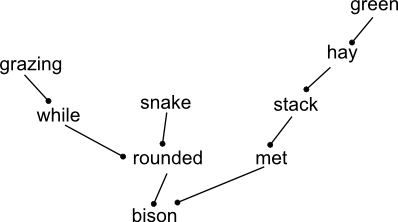
\includegraphics[scale=0.75]{ivans-bison-example.png}
\end{figure}
Notice that the links in the graph are directed, as the application operator is non-commutative, ie,
$$a \circ b \neq b \circ a .$$
\chapter{Memory organization}
\begin{flushright}
\emph{Computer science has only three ideas: cache, hash, trash}\\ --- Greg Ganger, CMU
\end{flushright}
\minitoc

\section{Associative memory}
\label{sec:associative-memory}

Associative recall can greatly facilitate inductive learning.

Sometimes fuzzy associations may be desirable.

The KB being in first-order logic poses problems for fuzzy associations.  It is unlike associative neural networks which may be closer to propositional logic.

\section{Efficient rule selection}

Given:\\
1. The goal (ie, the conclusion of the proof)\\
2. The premises (ie, facts residing in Working Memory)\\
Try to predict:\\
3. The rules involved in the proof

Each data point would be:\\
1.  goal (a grounded fact)\\
2.  premises (set of grounded facts)\\
3.  a rule used in the derivation of the goal

So the function we need is:\\
\{ fact \} $\times$ \{ set of facts \} $\rightarrow$ rule

Using multidimensional scaling, we can map a fact to its coordinates in a high-dimensional space.

Then we can partition the high-dimensional space into grids, and to each grid assign a bucket of rules.  We need some way to partition the high-dimensional space.  But we can also partition the space of data points into many categories?

\subsection{Hierarchical clustering of oracles}
\label{sec:hi-oracle}

\underconst
\chapter{Planning and acting}
\label{ch:planning-acting}
\minitoc

\section{``Procedural subsumes Declarative''}
\label{sec:proc-subsumes-decl}

So far, we have only talked about the \textbf{declarative} aspect of AGI.  Now we need to consider the \textbf{procedural} aspect.

It seems natural that the procedural system should subsume the declarative system:
\begin{figure}[H]
\centering
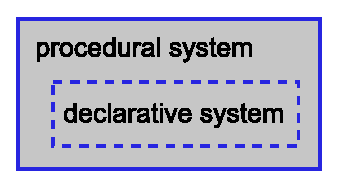
\includegraphics{Procedural-subsumes-Declarative-system.eps}
\end{figure}
\vspace{-0.5cm}

The procedural system communicates with the declarative system via various types of \textbf{querying}.  The declarative system itself has no means of performing actions;  its only function is question-answering.  There may be exceptions, but the general rule can be captured by the slogan \textit{``Procedural subsumes Declarative''}.

\section{The action language}
\label{sec:ActionLanguage}

We have represented declarative knowledge using a logical language; now we should represent procedural knowledge with a similar action language.

The following are examples of ``actions'':\\
1. say "hello"\\
2. open a file\\
3. print 1...100\\
4. repeat printing N until the user presses the Esc key

Do they sound like programming language tasks?  Thinking along this line, it seems advantageous that \textit{the action language should be a conventional programming language} such as C++, Java, Lisp,  Prolog, etc.

So the procedural system expresses actions in a programming language.  Those actions can be executed via the compiler or interpreter of that language.  In some situations, it is more convenient if the language can be interpreted.

The action output of the Procedural System can be of 3 forms:\\
1. a statement that is immediately interpreted and executed\\
2. a program that needs to be compiled\\
3. a program fragment that becomes part of the Procedural System

\#3 is actually a form of procedural learning.

\section{Procedural learning}
\label{sec:ProceduralLearning}

When the procedural language is complex, learning may be more difficult.  So there may be a need to restrict the procedural language.  %Secondly, there may be a need to put the learned procedures within a meta-controller framework so as to control them better.

Learned procedures can be inserted into the Procedural System at certain hook points.  Each hook point represents a context, for example ``We get here when the user presses the Esc key''.  The procedural learning algorithm should take such contexts into consideration.

``learn by being told'' is also applicable to procedural learning.

\section{Reinforcement learning} \index{reinforcement learning}
\label{sec:RL}

The goal of RL is to learn an optimal policy which is a function from the set of states to the set of actions:\\
\hspace*{1cm} $\pi: \mathbb{S} \rightarrow \mathbb{A}$.

RL can learn to:\\
1.  conversate with humans (eg in chat rooms)\\
2.  write programs\\
3.  crawl the web to learn things\\
and do all these without the need for human programming, so it is cost-effective.

See also \S\ref{sec:combine-DP-RL} on combining deductive planning and RL.

\subsection{Relational reinforcement learning}

(cf \citep*{Dzeroski1998}, \citep*{Dzeroski2001}, \citep*{Tadepalli2004}, \citep*{Driessens2005})

One problem with RL is that the number of states in a general intelligent agent is too large (in fact, infinite).  I suggest using FOL to describe the states so the formulation can be more compact.\\
A state would be a conjunction of ground literals, such as:\\
\hspace*{1cm} S1 = horny(john) $\wedge \; \neg$ good-looking(john) $\wedge$ has-money(john)\\
and the policy could be a rule that recommends an action from a state:\\
\hspace*{1cm} $\neg$ good-looking(X) $\wedge$ has-money(X) $\rightarrow$ try(X, buy-a-cybernetic-body)\\
Such a logical rule is not exactly a function, because:
\begin{compactenum}[1.]
\item More than one state can be true at the same time
\item If 2 states are both true and S2 $\supset$ S1, and\\
\hspace*{1cm} S1 $\rightarrow$ try(action1)\\
\hspace*{1cm} S2 $\rightarrow$ try(action2)\\
then both actions will be recommended when S2 is true.  We need a \textbf{conflict resolution} scheme to resolve this.\\
\{ TO-DO \} \\
\end{compactenum}

\subsection{RL and logical reasoning}

The relationship between RL and logical reasoning is very fascinating:  we can regard logical deduction as the task of searching for the proof of a query;  then RL can be used to perform deduction via learning the policy:\\
\hspace*{1cm} $\pi$ : search state $\mapsto$ search state.\\
From the previous section, we see that relational RL can vastly increase the expressive power of RL through generalization of states.  So the search states of the logical proof space can be generalized to what we call \textbf{cognitive states}, and the job of RL is to learn the policy:\\
\hspace*{1cm} $\pi$ : cognitive state $\mapsto$ cognitive state.

In this setting, the KB is part of the environment, and we'll have actions that manipulate the KB such as adding, subtracting, and searching KB items.

Thus, the entire logical reasoner can be implemented within RL.

The question now is how to represent cognitive states and their transitions.

\section{Means-ends analysis (MEA)}

MEA is a planning method proposed first by \citep*{Newell1960} for GPS (General Problem Solver).  They believed that MEA occurs in human problem solving.  It is  a \textit{forward} chaining feature-space\footnote{The feature space is similar to the state space except that a set of features only partially describe a state and thus can economically encompass many states.  This is a virtue in view of an agent's limited knowledge of the complex world.} search (ie, applying operators forwardly until the goal state is reached).  MEA selects a difference between the current state and the goal state, then selects an operator that may reduce the difference, and attempts to apply the operator.  If the operator's preconditions are not met, MEA recursively calls itself to transform the current state into one that meets those conditions.  If the conditions are met, MEA applies the operator and then recurse to transform the new state into the goal state (from \citep*{Langley1993}).

Wikipedia:  ``Note that, in order for MEA to be effective, the goal-seeking system must have a means of associating to any kind of detectable difference those actions that are relevant to reducing that difference.''

\{ TO-DO:  how to combine MEA with RL and deductive planning? \}

\section{Deductive planning}
\label{sec:deductive-planning}

A classical planning problem is represented by states and operators (actions).  Each operator has its precondition and effect.

In deductive planning based on situation calculus, actions are represented as terms, with the special predicates \code{do()} and \code{poss()}.

An advantage of deductive planning is that the Procedural System only needs to be an inference engine and nothing else.

One difficulty here is how to represent states, actions, preconditions, and effects;  especially actions.  I can put the cup on the table.  The current state is represented implicitly by all the facts in KB.  The actions are a special class of facts related to possibilities.  ``Water conducts electricity'' is a fact;  But ``water can conduct electricity'' is a possible action?  

Also, DP has a problem in that it only pursues one goal at a time.

\subsection{Example}

\begin{quote}
\emph{I try to kill Frank by tossing a radio in the bathtub while he is in it.  This may work because I know that water conducts electricity, and electricity can kill, etc.}
\end{quote}

Deductive planning allows the AGI to draw general knowledge from the KB to represent the planning problem:\\
\hspace*{1cm} goal = kill Frank\\
\hspace*{1cm} current state = Frank in bathtub, radio nearby\\
\hspace*{1cm} possible actions = toss radio into bathtub, slash Frank's wrist with a knife, etc\\
\hspace*{1cm} background knowledge = water conducts electricity, etc

\subsection{Combining reinforcement learning and deductive planning}
\label{sec:combine-DP-RL}

DP says:  ``If I do X, Y will probably happen as a result''.\\
RL says:  ``At state S, if I perform action A, the reward is probably high''.

We cannot simply have 2 planners co-existing -- the actions recommended by DP may conflict with those recommended by RL.  We may simply stipulate that the logical reasoner (since it is cognitively more sophisticated) has priority over RL.

RL may invoke DP for a recommendation of action.  When DP fails to find a recommendation, RL will act.


\chapter{Program synthesis}
\minitoc

The most critical milestone of our project is to create a system that can perform simple automated programming.  Traditional program synthesis systems are hard to use because:\\
\begin{compactenum}[1.]
\item  They require \textit{formal specifications} of program requirements, which are often as hard to write as the programs themselves, sometimes even harder.

\item  The proof search is \textit{too slow} for any problem of practical size, or the systems often require human interaction for guidance.\\
\end{compactenum}

My proposal to solve these two problems are, respectively:\\
\begin{compactenum}[1.]
\item  Allow \textbf{informal} specification of programming goals.  This means using (restricted) natural language, including vague / probabilistic language.

\item  In order to speed up the program search, it seems that the only viable solution is to use knowledge to guide the search.  This is something that has been recognized in the AI community for a long time --- no clever search algorithm or heuristic can improve the search significantly, without domain-specific background knowledge.  Machine learning can be used to acquire such knowledge, but it is often an extremely difficult problem in itself; and we are also talking about a large body of background knowledge.  As I have argued in \S\ref{sec:learn-by-being-told}, the most efficient way to acquire knowledge is to give up machine learning and simply \textbf{learn by being told}.\\
\end{compactenum}

As with many AI problems, the program synthesis problem can be construed as a search, and we have the usual choice of top-down and bottom-up. % I think the more promising approach is top-down but is this really true?

\section{Formal program synthesis}

\chapter{Value judgments}
\begin{flushright}
\emph{The real question is not whether machines think but whether men do.}\\
--- B F Skinner
\end{flushright}
\minitoc

\section{My stance on AGI friendliness}

I do not have a rigorous theory for AGI friendliness and I'd be very suspicious of any such theory.  But I believe that AGI technology should be made widely available to the general public, because the distribution of power is the best safeguard against abuses of AGI.

Other than that, the AGI should be subject to certain laws that prevent exploitation (eg, unlimited growth or taking up of physical resources).  That would be the job of governments.


\section{Sentient vs non-sentient AGI}

\chapter{Vision / perception}
\label{ch:vision}
\minitoc

Note:  This chapter is transferred from my older web site (2006), and needs some polishing.  Many links are broken.  It still represents my current view of how AGI vision should be achieved, but my focus is no longer on vision.

\section{Design philosophy}

The vision module has the following features:
\begin{enumerate}[\textbullet ]

\item \textbf{Analytical.} Visual recognition follows a reductionistic scheme in which visual objects are broken down into smaller components (3D $\rightarrow$ 2D $\rightarrow$ 1D $\rightarrow$ 0D). There is no "black-box" in this analytical scheme. 

\item \textbf{Holistic.} The intelligent agent has complete access to all visual details, down to the smallest features. However this does not mean that the system is flooded with irrelevant details � the attentional mechanism selects salient features in a scene, but the intelligent agent is free to focus attention on any minute detail. 

\item \textbf{Complete.} It has the complete range of visual functions to serve as the "eyes" of an intelligent agent. 

\item \textbf{Cognitive.} Visual recognition often involves reasoning. Therefore, the vision module interacts closely with the cognitive aspects of the intelligent agent. 
\end{enumerate}

\section{Relation between cognition and  vision}

\begin{compactenum}
	\item What Is general intelligence?
	\item The GI-vision approach
\end{compactenum}

\subsection{What is  general cognition?}

A fundamental idea of cognition is \emph{compression of information}.

Sensory experience in its raw form is like a long movie:

\begin{figure}[H]
\centering

\includegraphics[scale=0.6, bb=0 0 272 155]{Movie.eps}
\end{figure}

The Visual Module compresses this movie into a semi-symbolic representation. The Cognitive Module further compresses this information. 

\begin{figure}[H]
\centering
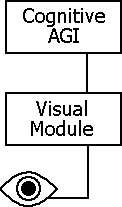
\includegraphics[scale=0.7, bb=0 0 122 207]{GI-Vision.PNG}
\end{figure}

Compression and achieved by (statistical) \emph{pattern recognition}. For example, in the "Lena" image

\begin{figure}[H]
\centering

\includegraphics[scale=0.7,bb=0 0 103 103]{Lena-Tiny.eps}
\end{figure}

the object in the center can be recognized as a "face".

GI is organized hierarchically, with higher abstraction at the top. At a very high level the Lena image may be compressed symbolically as "young woman wearing a hat".

The internal representation of a GI may be a data structure containing:
\begin{compactenum}
	\item objects
	\item properties of objects
	\item relations between objects
\end{compactenum}

Some examples:
\begin{compactenum}
	\item objects: "a face", "an apple", "the letter A"
	\item properties: "face.sex = female", "apple.color = red", "letter\_A.font = Times New Roman"
	\item relations: "hat \emph{above} face", "apple \emph{on} table"
\end{compactenum}

AGI is a system that can automatically invent concepts of new objects, properties, and relations. These new concepts are in turn applied to the internal representation. For example it may learn the new property "rectangular" by looking at a lot of rectangular shapes.

\subsection{The cognitive vision approach}

Vision is basically the problem of compressing the sensory input stream in a meaningful way.

\begin{figure}[H]
\centering

\includegraphics[scale=0.7,bb=0 0 103 103]{Lena-Tiny.eps} = "young woman wearing a hat"
\end{figure}

But there may be several \emph{levels} of representation.

As explained in the last section, each level of representation consists of:
\begin{compactenum}
	\item objects
	\item properties
	\item relations
\end{compactenum}

The pixel level is level 0 (not a representation).

 Level 1 consists of basic \emph{syntactic} features:
\begin{compactenum}
	\item edges / lines (includes straight lines and curves)
	\item regions of uniform color / intensity
	\item gradients of color / intensity
	\item textures
\end{compactenum}

These features are represented as objects. For example:
\begin{compactenum}
	\item object: curve1
	\item property: curve1.thickness = thin
	\item relation: curve1 \emph{connected-to} curve2
\end{compactenum}

At level 2 we may perform character recognition or 3D object recognition, and so on. 

The key thing here is that the vision problem is solved by  \emph{combining} GI and low-level processing. Once we have represented the image as objects + properties + relations, we can assume that a GI can handle it.

Level 1 processing is hand-programmed because it starts with pixels. Then we can rely on the GI to discover higher-level features (eg the concept "cube"). The GI will also allow us to hand-program some rules (known as \emph{knowledge insertion}), so  long periods of learning may be skipped.

\section{Machine vision --- general theory and background}

The background information on this page is adapted from [\hyperlink{ref}{Bruce, Green \& Georgeson 2003}] except otherwise stated.

\subsection{Background of general vision theories}

\subsubsection{Marr \& Nishihara (1978)}

Many people are familiar with Marr's vision theory so I won't go into details here.

This is a diagram explaining Marr's general vision framework [from \hyperlink{ref}{Herman Gomes' webpage}]:

\begin{figure}[H]
\centering
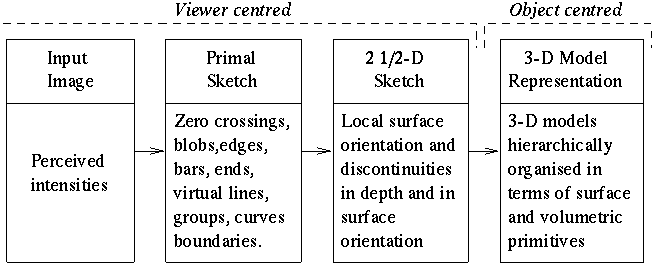
\includegraphics[scale=0.7,bb=0 0 653 267]{MarrVisionFramework.PNG}
\end{figure}

Another famous diagram from [\hyperlink{ref}{Marr \& Nishihara 1978}] [redrawn by \hyperlink{ref}{Herman Gomes}]:

\begin{figure}[H]
\centering
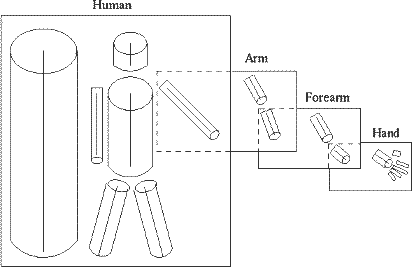
\includegraphics[scale=0.7,bb=0 0 414 269]{Marr3DModel.PNG}
\end{figure}

 Marr \& Nishihara's theory is restricted  to describing objects using a set of \emph{generalized cones} (after [Binford 1971]).

\subsubsection{Biederman and geons}

[\hyperlink{ref}{Biederman 1987}] (web page: \href{http://geon.usc.edu/~Ebiederman/}{geon.usc.edu/\textasciitilde biederman}) proposed the "recognition by components" theory, which is closely related to Marr and Nishihara's earlier theory. In Biederman's theory, complex objects are described as spatial arrangements of basic component parts known as "geons". Geons are defined by properties that are invariant over different views. Some example geons are [taken from \hyperlink{ref}{Kirkpatrick}'s web page]:

\begin{figure}[H]
\centering
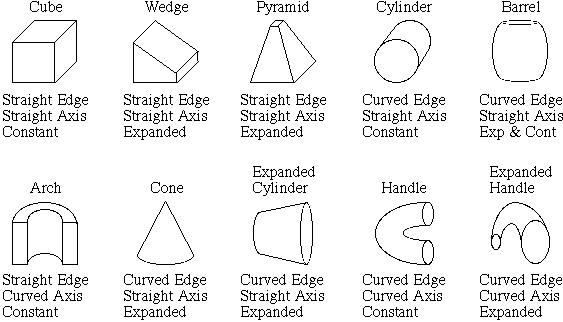
\includegraphics[scale=0.7,bb=0 0 653 322]{geons.PNG}
\end{figure}

In particular, [\hyperlink{ref}{Biederman \& Hummel 1992}] proposed a neural network system to recognize geon-based objects:

\begin{figure}[H]
\centering
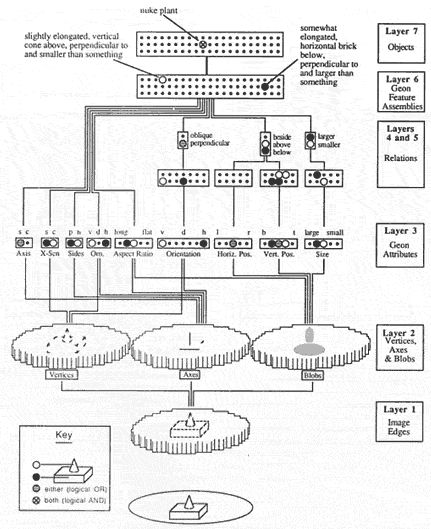
\includegraphics[scale=0.6,bb=0 0 431 529]{BiedermanHummelNN.PNG}
\end{figure}

\subsection{Our approach}

\subsubsection{Re Marr's \& Biederman's theories}

Our approach roughly conforms to Marr's framework of  "primal sketch $\rightarrow$ 2.5D $\rightarrow$ 3D" reduction, but we describe the reduction as "0D $\rightarrow$ 1D $\rightarrow$ 2D $\rightarrow$ 3D". It may not be such a big difference, so I'll skip the discussion of this issue.

Another similarity with Marr is that I think the high-level representation is 3D in nature. But I do not restrict the representation to generalized cones only. My theory is that any 3D object can be defined by 2D surfaces, and this theory is not restricted to generalized cones or Biederman's geons.

The following examples may convince you that some shapes are not representable by common geons:

\begin{figure}[H]
\centering
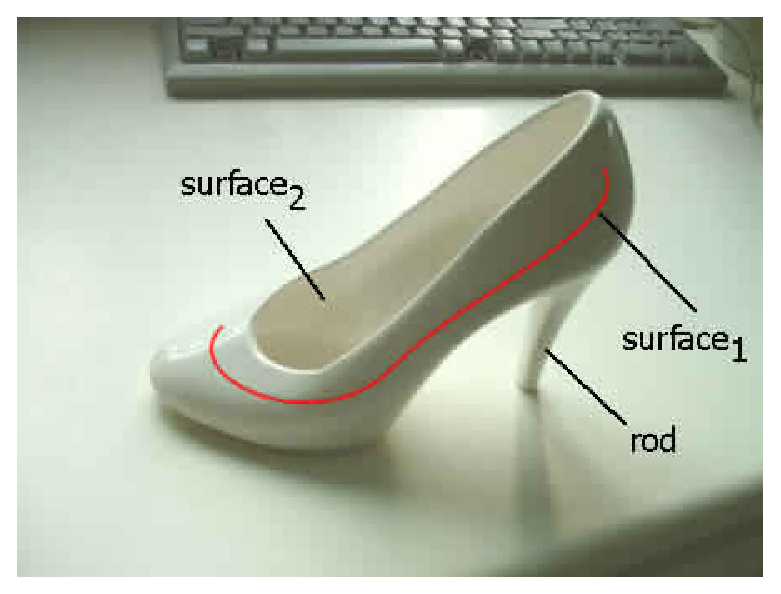
\includegraphics[scale=0.7,bb=0 0 448 336]{HighHeelAnalysis.eps}
\end{figure}

\begin{figure}[H]
\centering
\includegraphics[scale=0.7,bb=0 0 448 336]{ToiletRollAnalysis.eps}
\end{figure}

\begin{figure}[H]
\centering
\includegraphics[scale=0.7,bb=0 0 448 336]{RabitAnalysis.eps}
\end{figure}

In all of the above cases, the objects have parts that are defined by some irregular surfaces. The geon theory may fail in such cases because Biederman et al use neural networks to learn the geons, and the geons are \emph{statistically} characterized by  vertices, blobs, and axes. This kind of learning may be slow and recognition may be erratic. What we need is a more robust theory that can represent \emph{any} 3D shape. The solution is to use \emph{logical rules} to define geons in terms of 2D lines and junctions:

\begin{figure}[H]
\centering
\includegraphics[scale=0.6, bb=0 0 346 228]{PolygonDecomposition.PNG}
\end{figure}

This method is more robust and can recognize things other than common geons, such as the highheel.

\subsubsection{Shape from shading and from texture}

A number of algorithms have been developed to recover "shape from shading" with the aim of describing the 3D shape given only the pattern of reflected light intensities (for example \hyperlink{ref}{Horn \& Brooks 1989}), and "shape from texture". Shape from texture is a particularly hard problem so we will handle it later.

But  the framework of 3-2-1-0D reduction still holds for "shape-from-X". It is relatively easy to describe 3D shapes in terms of  2D surfaces, and 2D surfaces in terms of 1D contours; but it is very difficult to jump from a set of pixels straight to a 3D description. This is probably why many prior vision theories failed.

For example, to recognize the  nose, one should first recognize the shades and highlights and contours as 2D/1D features:

\begin{figure}[H]
\centering
\includegraphics[scale=0.7,bb=0 0 336 448]{BeethovenAnalysis.eps}
\end{figure}

The conjunction of these 2D/1D elements allows us to recognize that the nose is a protrusion from the face, and its particular shape is jointly defined by the shapes of  2D/1D elements. It seems that a common mistake is to assume that the brain immediately recognizes the nose as a 3D shape  from pixel-level data, without going through the intermediate stages, because the brain is usually unconscious of those intermediate stages.

Recognizing shading as 2D features will require special algorithms (so does recognizing textures). At first we will focus on using exclusively edge detection (contours) to recognize objects.

\subsubsection{References}

[Biederman 1987] \emph{Recognition by components: A theory of human image understanding}. Psychological Review, 94, 115-145

[Biederman \& Hummel 1992] \emph{Dynamic binding in a neural network for shape recognition}. Psychological Review 99, 480-517 

[Binford 1971] \emph{Visual perception by computer}. Paper presented at the IEEE Conference on Systems and Control, December 1971, Miami

[Bruce, Green \& Georgeson 2003] \emph{Visual Perception --- Physiology, Psychology and Ecology}, Psychology Press, NY

[Gomes 2000] Herman Gomes' web page: \emph{Marr's Theory: From primal sketch to 3-D models}, \href{http://homepages.inf.ed.ac.uk/rbf/CVonline/LOCAL_COPIES/GOMES1/marr.html}{http://homepages.inf.ed.ac.uk/rbf/CVonline/LOCAL\_COPIES/GOMES1/marr.html}

[Horn \& Brooks 1989] \emph{Shape from shading}. MIT Press, Cambridge, MA

[Kirkpatrick K] Web page on object recognition \href{http://www.pigeon.psy.tufts.edu/avc/print/kirkpatrick/kirkpatrick_figprint.htm}{http://www.pigeon.psy.tufts.edu/avc/print/kirkpatrick/kirkpatrick\_figprint.htm}

[Marr \& Nishihara 1978] \emph{Representation and recognition of the spatial organization of 3D shapes}. Proceeding of the Royal Society of London, series B, 200, 269-294 

\section{Requirements of general vision}

\includegraphics[bb=0 0 40 40]{UnderConst.png}

\section{Basic vision scheme}

Our approach to solving the general vision problem is to combine vision with GI (general intelligence). See \href{Vis-Cognition.htm}{an introduction to GI-vision}.

The basic tenets of my vision theory are:
\begin{compactenum}
	\item  Break down the image via 3D-2D-1D-0D primitives
	\item  Apply  machine learning to represent the image symbolically
\end{compactenum}

I have thought about the vision problem for 1-2 years and studied many real images to conclude that "everything under the sun" can be recognized by this method. A  paper will be published to explain the theory in detail.
\underconst
\begin{compactenum}
	\item \hyperlink{3210DReduction}{3-2-1-0D reduction}
	\item \hyperlink{LogicalRepresentation}{Logical representation}
	\item \hyperlink{MachineLearning}{Machine learning}
	\item \hyperlink{Example}{Example: quadrilateral}
	\item \hyperlink{ApproximateRecognition}{Approximate recognition and feedback}
	\item \hyperlink{Attention}{Searchlight attention}
	\item \hyperlink{Relations}{Relations between objects}
	\item \hyperlink{Architecture}{Architecture of the vision module}
\end{compactenum}

\subsection{3-2-1-0D reduction}

The premise is that any 3D object (or its "geon-like" components) can be defined by  2D surfaces, which are in turn defined by 1D lines. Please refer to \href{Vis-Background.htm}{General vision theory and background} for the justification of this point.

\begin{figure}[H]
\centering
\includegraphics[scale=0.6, bb=0 0 346 228]{PolygonDecomposition.PNG}
\end{figure}

The image is first broken down into 0D/1D primitives (such as edgels and lines). Then 2D elements are recognized (such as regions and surfaces). Then 3D objects are recognized (blocks, 3D geons, etc).

The decompositions are represented by graphical data structures (ie nodes and links). Nodes are primitive elements; Links represent the spatial relations between them.

Details of \href{Vis-3210D-Reduction.htm}{3-2-1-0D reduction}.

Our 1D-2D levels may coincide with David Marr's primal sketch level. Here we reframe these levels under the \href{Vis-PrimalSketch.htm}{primal sketch} framework.

\subsection{Logical representation}

The first step is to transform the image to a logical representation:

\begin{figure}[H]
\centering
\includegraphics[scale=0.8, bb=0 0 568 326]{VisioLogicalTransform.eps}
\end{figure}

On the left hand side is the image; we have applied  Sobel edge detection. On the right hand side is the logical representation. L1,L2,L3... = lines, J1,J2,J3... = junctions. The blue lines represent how the elements are connected. Other details at the background have not been represented.

For simple, uncluttered scenes, this scheme will work fine. The idea is that every detail, no matter how irregular, would be represented using this logical representation (using elements such as blobs and shades in addition to lines, junctions, etc).

This approach requires a lot of patience, but ultimately we would be able to analyse everything in the world. Other approaches such as neural network or SIFT are not as general or comprehensive.

We may use neural networks at the lowest level for recognizing "edgels". Then the next stage is to join the edgels to recognize longer lines.

\subsection{Machine learning}

What we need is a special kind of machine learning known as inductive learning (as opposed to deductive learning). In inductive learning a system tries to induce \emph{general rules} from a set of observed instances ("learning by examples").

There should be an underlying knowledge representation (KR) or  "calculus" that encompasses what kinds of rules are possible. The most common KR scheme is first-order predicate logic, often abbreviated as FOL (first order logic). Other options include: neural networks, semantic networks, conceptual graphs, Bayesian networks, etc.

It is not easy to determine what kind of KR is adequate for our task at hand (visual recognition). Therefore we start with something simple and similar to FOL and see if it needs to be expanded or modified.

Details of \href{Vis-InductiveLearning.htm}{inductive learning}. 

\subsection{Example: quadrilateral}

Any figure with 4 sides (straight lines).

Define the predicate \texttt{Terminates(edge,vertex)}  to indicate when an edge terminates with a vertex.

\begin{figure}[H]
\centering
\includegraphics[scale=0.6, bb=0 0 608 340]{Quadrilateral.eps}
\end{figure}

This results in the set of logical statements:
\begin{quote}

\texttt{Terminates(edge$_1$,vertex$_1$) = true
\\
    Terminates(edge$_1$,vertex$_2$) = true
\\
    Terminates(edge$_2$,vertex$_2$) = true 
\\
    Terminates(edge$_2$,vertex$_3$) = true 
\\
    Terminates(edge$_3$,vertex$_3$) = true
\\
    Terminates(edge$_3$,vertex$_4$) = true 
\\
    Terminates(edge$_4$,vertex$_4$) = true 
\\
    Terminates(edge$_4$,vertex$_1$) = true
  }
\end{quote}

Perhaps, we can introduce a new predicate \texttt{Connects(edge,vertex$_1$,vertex$_2$)} to simplify the above to:
\begin{quote}

\texttt{Connects(edge$_1$,vertex$_1$,vertex$_2$) = true
\\
    Connects(edge$_2$,vertex$_2$,vertex$_3$) = true
\\
    Connects(edge$_3$,vertex$_3$,vertex$_4$) = true
\\
    Connects(edge$_4$,vertex$_4$,vertex$_1$) = true}
\end{quote}

Assuming that the "universe"  is a connected graph that the system is currently paying attention to, now we can easily define the 0-ary predicate \texttt{Quadrilateral()} using \emph{typed logic}:
\begin{quote}

\texttt{Quadrilateral() :-}
\begin{quote}

\texttt{$\exists $ e$_1$:edge
\\
      $\exists $ e$_2$:edge
\\
      $\exists $ e$_3$:edge
\\
      $\exists $ e$_4$:edge
\\
      $\exists $ v$_1$:vertex
\\
      $\exists $ v$_2$:vertex
\\
      $\exists $ v$_3$:vertex
\\
      $\exists $ v$_4$:vertex
\\
      Connects(e$_1$,v$_1$,v$_2$) $\wedge$
\\
      Connects(e$_2$,v$_2$,v$_3$) $\wedge$
\\
      Connects(e$_3$,v$_3$,v$_4$) $\wedge$
\\
    Connects(e$_4$,v$_4$,v$_1$)}
\end{quote}
\end{quote}

This is just an example. Please refer to this page concerning  various issues of \href{Vis-InductiveLearning.htm}{inductive learning}. Some other issues specific to vision are discussed as follows.

\subsection{Approximate recognition and feedback}

One problem is that primitive features  are often fuzzy and should be approximately recognized.

For example, in the image below, 2 edges and 1 vertex are almost invisible, yet given the current \emph{context} they should be interpreted as edges and vertex. The context is important because very weak features would be regarded as noise otherwise:

\begin{figure}[H]
\centering
\includegraphics[scale=0.8, bb=0 0 240 320]{CubeMissingEdge.eps}
\end{figure}

The feedback mechanism should work this way: When the Recognizer finds that a concept is "almost" recognized (eg with the majority of conjuncts being true), it will select the remaining features that are not yet matched and send them to the lower-level Recognizer, which would then lower its \emph{threshold} for recognizing those features.

This requires 2 things:
\begin{compactenum}
	\item The Recognizer  should measure a \emph{degree of certainty} associated with each feature being recognized.
	\item  The Recognizer  at the lower level should be able to use an feedback cue to look for certain features. This may require performing an "inversion" of the cue.
\end{compactenum}

A detailed explanation of the feedback mechanism will be presented soon.
\underconst

\subsection{Searchlight attention}

Another problem is that real world images are often composed of many cluttered elements, so we need to use a "searchlight" to look for individual objects in a cluttered scene.

Searchlight attention is closely related to the feedback mechanism outlined above. Due to limited computational resources we can only extract features within a "fovea" of attention. If a concept is detected to be "almost" complete, the searchlight will direct the fovea to focus on  areas that are likely to complete the concept, with a concomitant decrease of attention to other areas.

This requires the searchlight to know \emph{where} to search for the feedback cue. In a sense this also requires inversion of the cue.

\subsection{Relations between objects}

The vision system not only has to recognize individual objects, but also relations among them (represented as links).

The way to achieve this is to pay attention to individual objects \emph{sequentially}. Relations are then recognized by the identities of the objects in the sequence and by how the searchlight moved.

In our logical formulation, an object is recognized by a 0-ary predicate such as \texttt{Cube$_1$()}. Then we have to bring this object to the \emph{next} level of recognition, where it is represented by a variable such as \texttt{cube$_1$}. Only then we would be allowed to denote a relation like \texttt{Above(cube$_1$,cube$_2$)} at this level.

Recognition at each level is \emph{independent} of recognition at other levels, except for the feedback mechanism.

The "main loop" of the Recognizer would be using the searchlight to scan around the image, and recognizing individual objects. When the searchlight moves, its movement will be recorded and later used to form the link between the current object and the next object.

\subsection{Architecture of the vision module}

\begin{figure}[H]
\centering
\includegraphics[scale=0.6, bb=0 0 726 380]{VisionArchitecture.PNG}
\end{figure}

The operation of the above module is typical of a rule-based system, except that there is a "loop" in the lower right corner that repeats the pattern matching process at multiple levels. What this means is that the raw sensory experience goes through multiple stages of memory consolidation via pattern matching. For details please refer to \href{GI-MemorySystems.htm}{Memory systems}. 

This architecture has to be integrated with the larger GI (general intelligence) framework, to form a complete intelligent agent. Please refer to \href{GI-architecture.htm}{GI architecture}.

\section{Details of  3-2-1-0D reduction}

An illustrated example ("cube") is \href{Vis-Example.htm}{here} (incomplete)
 
\underconst

The following is a very tentative outline, the order of steps may be wrong and additional steps may be needed...

\subsection{Stage 1: 1D Analysis }

1. Edge detection --- distinguish between single-pixel lines and thick lines.

2. \href{Vis-1DTaxonomy.htm}{Classification of 1D lines}: straight lines, curves, junctions. From this point on the representation is a collection of discrete lines and junctions: qualitative / structural rather than quantitative / spatial / continuous.

3. Good continuation --- line / curve completion.

\begin{figure}[H]
\centering
\includegraphics[scale=0.6, bb=0 0 265 109]{GoodContinuation.eps}
\end{figure}

4. Contour simplification --- the image is represented by both simple and detailed contours (allowing redundency in representation).

\begin{figure}[H]
\centering
\includegraphics[scale=0.6, bb=0 0 346 120]{ContourSimplification.eps}
\end{figure}

Some things can be recognized at this stage: text, handwriting, 1D graphics.

\subsection{Stage 2: 2D Analysis}

5. Characterization of regions according to color, shading or textures (segmentation).

6. Classification of 2D shapes

\underconst

7. Extract gestalt-induced contours --- (a) numerous small, identical / similar elements may induce contours; (b) the absence of features induces "invisible" contours

\begin{figure}[H]
\centering
\includegraphics[scale=0.6, bb=0 0 290 102]{GestaltContours.PNG}
\end{figure}

8. Deal with occlusion.

Some 2D graphics may be recognized at this stage.

\subsection{Stage 3: 3D Analysis}

9. \href{Vis-3DTaxonomy.htm}{Classification of 3D lines / surfaces}.

10. Identify objects according to templates or algorithms. The question is how to define an object such as the object classes "bottle", "books", "faces", etc.

\section{Primal sketch project}

\subsection{Background}

According to Marr, the primal sketch represents changes in light intensity occuring over space in the image. It also organises these local descriptions of intensity change into a 2D representation of image regions and the boundaries between them.

Specifically, the primal sketch may include elements such as edges (curves or straight lines), color blobs, ends, junctions (of edges), texons, etc.

Marr's vision scheme consists of 3 levels:
\begin{compactenum}
	\item primal sketch
	\item 2.5D
	\item 3D
\end{compactenum}

My \href{Vis-BasicScheme.htm}{vision scheme} is slightly different which goes from 3D, 2D to 1D. This difference may not be all that important; what is important is how best to recognize features at various levels, from a computational viewpoint. The primal sketch is an essential stage of any complete vision system.

What I propose is that the output of the primal sketch should be represented as a symbolic web with links that are logical predicates. Developing such a low-level layer would make a tremendous contribution towards computer vision.

\subsection{What we're trying to do }

\subsubsection{1. Obtaining the primal sketch }

One solution to the primal sketch problem (I have not surveyed the topic completely) is presented in [\hyperlink{Ref}{Gao, Zhu \& Wu 2006}], "Primal Sketch: Integrating Texture and Structure" (\href{http://www.stat.ucla.edu/~sczhu/papers/primal_sketch.pdf}{pdf}), by researchers in the UCLA Center for Image and Vision Science.

As explained in the paper, an input image is separated into 2 regimes, one "sketchable" and the other "non-sketchable". The sketchable regime is one of low entropy where the image can be represented by a sparse-coding sum of primitive features; the non-sketchable regime is of relatively higher entropy where sparse-coding is no longer practical and those areas of the image should be represented as \emph{textures}.

In our project we were trying to deal with the type of low level feature extraction in the sketchable regime, while temporarily ignoring textures. I'm currently trying to have a collaboration with the UCLA group or possibly license their technology.

\subsubsection{2. Output an attributed graph}

After obtaining the primal sketch, the second task is to represent the image as an attributed graph. This has been partly accomplished in [\hyperlink{Ref}{Han \& Zhu 2005}], \emph{Bottom-up/Top-down Parsing with Attributed Graph Grammar} (\href{http://www.stat.ucla.edu/~sczhu/papers/PAMI_Grammar_rectangle.pdf}{pdf}), for some simple shapes.

The goal of our project is to output attributed graphs similar to the above kind for all sorts of images. The expressiveness of the attributed graph may be comparable to that of first-order predicate logic.

 Then the next step is to delegate the tasks of recognition and inference to an intelligent agent or cognitive architecture.

\subsubsection{3. Handover to intelligent agent}

The following tasks may be handled by the intelligent agent:
\begin{compactenum}
	\item pattern recognition
	\item attentional mechanism (eg focusing attention to various features or objects)
	\item learning of concepts and facts (declarative and episodic memory)
	\item complex inference (for example, a chair is "anything that can be sat on", may involve procedural memory)
\end{compactenum}

The division of labor can avoid repeating these tasks for vision and for general cognition.

Currently we are considering the following intelligent agents for integration with vision:
\begin{compactenum}
	\item Novamente (has an architecture integrating perception and cognition)
	\item Soar (has provisions for sensory perception)
	\item Cyc (depends on its proprietary inference engine)
	\item ACT-R
	\item EPIC
	\item IDA (intelligent distribution agent, Stan Franklin)
\end{compactenum}

Basically any general cognitive architecture that can handle sensory perception, can use our vision module.

\subsubsection{References}

[Guo,  Zhu \& Wu 2006] \emph{Primal Sketch: Integrating Texture and Structure}, 
Computer Vision and Image Understanding, 2006 (Accepted for the Special Issue on Generative Model Based Vision) (\href{http://www.stat.ucla.edu/~sczhu/papers/primal_sketch.pdf}{pdf})

[Han \& Zhu 2005] \emph{Bottom-up/Top-down Image Parsing with Attribute Graph Grammar}, 
Statistical preprint, 2005. Submitted to PAMI (\href{http://www.stat.ucla.edu/~sczhu/papers/PAMI_Grammar_rectangle.pdf}{pdf}) 

\section{Classification of 1D Shapes}

Here I attempt to classify all 1D shapes (contours) into primitive elements (lines, curves, junctions).

My view is that the vision problem (especially the recognition of 3D objects) can be solved via a 3D $\rightarrow$ 2D  $\rightarrow$ 1D process. All  3D objects can be defined by 2D elements (surfaces), and all 2D shapes (areas) can be defined by 1D contours.

\subsection{Main Classes}

All 1D shapes can be decomposed into: 

\begin{figure}[H]
\centering
\includegraphics[scale=0.7, bb=0 0 404 87]{1DClasses.PNG}
\end{figure}

\textbf{Properties:} (thickness, color, texture)

\subsection{1. Straight Lines}

\textbf{Properties:} (position, length, orientation, end points)

\subsection{2. Curves}

4 subtypes:

\subsubsection{1. Simple Curves}

Curves with no inflections:

\begin{figure}[H]
\centering
\includegraphics[scale=0.7, bb=0 0 325 42]{CurvesClasses.PNG}
\end{figure}

\textbf{Properties:} (position, length, orientation, end points, curvature)

\subsubsection{2. Ellipses/Circles}

\begin{figure}[H]
\centering
\includegraphics[scale=0.7, bb=0 0 91 62]{EllipsesClasses.PNG}
\end{figure}

\textbf{Properties:} (position, orientation, size, axes ratio)

\subsubsection{3. Complex Curves}

\begin{figure}[H]
\centering
\includegraphics[scale=0.7, bb=0 0 198 77]{ComplexCurves.PNG}
\end{figure}

\textbf{Properties:} (position, length, end points, \# of inflections, curvatures) 

\subsubsection{4. Complex Loops}

\begin{figure}[H]
\centering
\includegraphics[scale=0.75, bb=0 0 197 108]{ComplexLoops.PNG}
\end{figure}

\textbf{Properties:} (position, area, shape description, \# of inflections)

\subsection{3. Junctions}

\textbf{Properties:} (position, \# of lines, angles) 

3 subtypes:

\subsubsection{1. L}

\begin{figure}[H]
\centering
\includegraphics[scale=0.7, bb=0 0 239 40]{Junctions-L.PNG}
\end{figure}

\subsubsection{2. T}

\begin{figure}[H]
\centering
\includegraphics[scale=0.7, bb=0 0 232 40]{Junctions-T.PNG}
\end{figure}

\subsubsection{3. Y }

\begin{figure}[H]
\centering
\includegraphics[scale=0.7, bb=0 0 220 118]{Junctions-Y.PNG}
\end{figure}

\subsubsection{4. X}

\begin{figure}[H]
\centering
\includegraphics[scale=0.7, bb=0 0 230 110]{Junctions-X.PNG}
\end{figure}

May have $>$4 lines of convergence.

\subsection{Examples}

The following examples illustrate the concept of \textbf{self-aggregation}, which means edgel detectors (or "neurons") aggregating with others with similar attributes such as color, orientation, etc.

A line with a slight bend: (the bending is noticed even though it is very slight, because the A \& B parts are very straight in contrast):

\begin{figure}[H]
\centering
\includegraphics[scale=0.7, bb=0 0 260 39]{Line1.PNG}
\end{figure}

This line has many bends but is still recognized as a continuous line: 

\begin{figure}[H]
\centering
\includegraphics[scale=0.7, bb=0 0 182 38]{Line2.PNG}
\end{figure}

For the following line, a simple algorithm may classify it as a curve, but people will describe it as: two slightly curved lines A \& C, bending at a point B. This illustrates the context-dependent aspect of human vision.

\begin{figure}[H]
\centering
\includegraphics[scale=0.7, bb=0 0 272 132]{Line3.PNG}
\end{figure}

The following is yet another context-dependent example: we see 2 "shaky" but straight lines bending at an angle.

\begin{figure}[H]
\centering
\includegraphics[scale=0.7, bb=0 0 170 66]{Line4.PNG}
\end{figure}

What is a "straight" line is relative: B is straighter than A but in the above context A is also considered a straight line. 

\begin{figure}[H]
\centering
\includegraphics[scale=0.7, bb=0 0 219 32]{Line7.PNG}
\end{figure}

People will describe the following as a regular "sine" curve:

\begin{figure}[H]
\centering
\includegraphics[scale=0.7, bb=0 0 199 35]{Line5.PNG}
\end{figure}

This is also a simple curve that people can describe with basic features such as crest and trough and being smooth:

\begin{figure}[H]
\centering
\includegraphics[scale=0.7, bb=0 0 310 72]{Line6.PNG}
\end{figure}

People can also characterize line junctions with special attributes, eg a "smooth" junction:

\begin{figure}[H]
\centering
\includegraphics[scale=0.7, bb=0 0 228 78]{Line8.PNG}
\end{figure}

This can be considered as  1 line with 2 colors:

\begin{figure}[H]
\centering
\includegraphics[scale=0.7, bb=0 0 248 6]{Line9.eps}
\end{figure}

This is also considered a simple curve with internal texture:

\begin{figure}[H]
\centering
\includegraphics[scale=0.7, bb=0 0 200 40]{Line10.PNG}
\end{figure}

\underconst

\section{Classification of 2D features}

\underconst

\section{Classification of 3D Shapes}

There are a limited number of possible 3D contours and junctions. The technique of labeling all contours and junctions consistently is known as \emph{relaxation labeling} and has grown into a large area of work.

We should work out the rules of arbitrary 3D object construction...

\underconst

\subsection{3D Edges}

\begin{figure}[H]
\centering
\includegraphics[scale=0.7, bb=0 0 293 276]{3DContours.PNG}
\end{figure}

D = discontinuity of distance of object, discontinuity of normal of object surface

DC = discontinuity of distance of object, continuous normal of object surface

N = discontinuity of normal of object surface 

R = change of reflectance

S = shadow

Each type of contour has its characteristics such as shading. Such characteristics help to infer its type.

\subsection{3D Junctions }

There are 16 topologically possible line junctions in the "trihedral blocks world":

\begin{figure}[H]
\centering
\includegraphics[scale=0.7, bb=0 0 499 357]{16Junctions.PNG}
\end{figure}

+ and - indicates whether a crease is convex or concave, respectively. An arrow indicates a "blade" formed by a discontinuity of distance (same as the D-type contour above). The direction of the arrow indicates which side is the \emph{occluding} surface, which by convention is to the right.

We should extend this analysis to arbitrary 3D shapes.

\section{Inductive learning for vision}

Inductive logic programming seems to be the harder part of our project (in fact ILP is considered one of the hardest areas in computer science!)

\subsection{Background to ILP (inductive logic programming)}

\subsubsection{Books and internet resources}
\begin{compactenum}
	\item \emph{Machine Learning} [Mitchell 1997] \emph{}has a chapter on "Learning Sets of Rules" which is a good introduction.
	\item \emph{AI: A Modern Approach} talks about ILP in chapter 19
	\item {\normalsize This 1994 book by N. Lavrac and S. Dzeroski is free for download: \textit{\href{http://www-ai.ijs.si/SasoDzeroski/ILPBook/}{Inductive Logic Programming: Techniques and Applications}.}}
	\item Stephen H Muggleton's website on ILP: \href{http://www.doc.ic.ac.uk/~shm/}{www.doc.ic.ac.uk/\textasciitilde shm/}
	\item Peter A Flach's website: \href{http://www.cs.bris.ac.uk/~flach/}{www.cs.bris.ac.uk/\textasciitilde flach} and his PowerPoint on \href{http://macflach.cs.bris.ac.uk/~flach/presentations/CL2000HTML/CL2000.ppt}{Knowledge Representation and ILP}.
	\item many more...
\end{compactenum}

\subsubsection{A simple ILP example}

To learn the relation \texttt{Daughter(x,y)}.

A database may have the following facts:
\begin{quote}

\texttt{Male(mary) = false
\\
    Female(mary) = true
\\
    Mother(mary, louise) = true
\\
    Father(mary, bob) = true
\\
    Daughter(bob, mary) = true
\\}etc......
\end{quote}

After presenting a large number of such facts,this rule may be learned:
\begin{quote}

\texttt{IF Father(y,x) $\wedge$ Female(y) THEN Daughter(x,y)}
\end{quote}

\subsubsection{Existing ILP software}
\begin{compactenum}
	\item FOIL
	\item  CIGOL ('logic' spelt backwards)
	\item GOLEM
	\item  PROGOL
	\item LINUS
	\item etc...
\end{compactenum}

\subsection{Special concerns related to vision}

The "fovea" focuses on a particular area or scale of an image. Low-level feature extraction results in a graphical representation of the scene. The nodes and links of this graphical representation is then converted to a set of logical statements. This set is then taken to be the "model" (possible world) of the logic.

Low-level feature extraction has to use the searchlight mechanism to discover the spatial relations among features, and then outputs a graphical / logical representation for the next level. The "universe" of the logic at each level is distinct from each other.

\subsection{Why use logic?}

 Our scheme is to reduce 3D to 2D to 1D to 0D. Along this route, many concepts need to be defined:
\begin{compactenum}
	\item  First, we have the image decomposed into edgels, which are the lowest-level features.
	\item  Then we define "lines" and "curves" as collections of contiguous edgels.
\\
    (From 0D to 1D: line = conjunction of edgels)
	\item  Then we define "polygons", "parallelograms", "squares", etc as collections of lines.
\\
    (From 1D to 2D: surface = conjunction of lines) 
	\item  Then we can define "cylinders", "blocks", etc as collection of surfaces.
\\
    (From 2D to 3D: volume = conjunction of surfaces)
	\item Then we define objects such as "bicycles", "wheels", etc as composed of primitive geons.
\end{compactenum}

If we can enter all these things as rules in a knowledgebase, we have a vision system that operates by the rules. Our strategy is to encode these rules as \emph{logical formulas}.

\subsubsection{Why not neural networks? }

The use of logic to represent rules (definitions) has a tremendous advantage over neural networks. For example, a quadrilateral is defined as any figure with 4 sides. Quadrilaterals can appear in all sizes and shapes, yet we have no problem recognizing any of them. With predicate logic, we can easily define a quadrilateral in terms of edges and vertices (an example is given in \href{Vis-BasicScheme.htm}{Vision scheme}). The resulting formula is very succinct and is capable of covering all possible cases (ie it has low algorithmic complexity).

On the other hand, in neural networks we have to learn the concept of quadrilaterals in a high dimensional space populated with many instances of quadrilaterals. Such a \emph{statistical} learning method continually "molds" the classification space into the right shape, with incremental steps, which is extremely inefficient and prone to errors. In other words, it fails to reduce algorithmic complexity significantly.

The essense of logic is that it can represent \emph{objects} and their \emph{relations}. Objects are variables and relations are predicates. The use of variables allows logic to represent many things \emph{succinctly}. For example I can use the predicate \texttt{Kicks(x,y)} to mean x kicks y. The predicate can be used to denote "boy kicks ball", "girl kicks dog", or "John kicks Mary" even though these events are very dissimilar. Thus the great expressiveness of predicate logic. Most artificial neural networks nowadays cannot express things with variables.

You may argue that the brain is a neural network and so they must be capable of achieving vision and cognition. I guess the answer is that the brain probably uses neurons to perform some sort of symbolic/logical computations, rather than statistical learning as many neuroscientists now assume. Unfortunately how the cortex performs computation is still a \emph{terra incognita}.

\subsection{What's the use of inductive learning?}

For a very simple vision system, inductive learning is not needed. All we need is to  patiently enter  definitions of shapes / objects into a logical knowledgebase. Then the system can recognize those things. 

Inductive learning is needed for 2 purposes:
\begin{compactenum}
	\item  teaching by "show and tell";
	\item  automatically discovering useful concepts.
\end{compactenum}

\subsubsection{"Show and tell"}

It is far easier to show the computer a number of examples of an object (eg "pineapple") than to explicitly define the general appearance of that object. The inductive learner will automatically generalize from the exemplars.

\begin{figure}[H]
\centering
\includegraphics[scale=0.7,bb=0 0 628 218]{Fruits.eps}
\end{figure}

\subsubsection{Automatic discovery of useful concepts}

This is an advanced topic, but of great practical value. A "useful" concept is one that helps meaningfully to characterize a broad class of objects. For example the concept of "leaf" may characterize the leaves often attached to many types of fruits, and may also apply to flowers and trees. So it is a useful concept.

Another useful concept is "parallelogram" which often occurs in the views of rectangular blocks. If we do not use the concept of parallelogram then the description of rectangular blocks may become cumbersome.

 In other words, a useful concept reduces description lengths. But if we are talking about the total description length of a knowledgebase, then the discovery of "good" concepts requires global searching. This is therefore a computational hard problem. 

\subsection{Inductive learning methods}

\underconst

We are currently looking for researchers in ILP to collaborate with us to develop the Inductive Learner...

\subsection{Outstanding questions}

Do we need some special inference operations outside of predicate logic? Such as stochastic logic?

When doing higher-level recognition, does the Recognizer need to be aware of the constituents of high-level features? Eg, that a line is a collection of edgels?

\section{Depth / distance estimation}

\underconst

\section{Motion and event detection}

\underconst

\section{Texture}

\underconst

\section{Stereopsis}

\underconst

\section{Sample images}

Sample images are currently hosted at:\\
\hspace*{1cm} http://www.geocities.com/genericai/Vis-SampleImages.htm
but the site will soon be closed (around October 2009).  I will try to relocate them somewhere.

\chapter{Implementation}

\begin{flushright}
\emph{The sooner you start coding your program the longer it's going to take}\\
--- H F Ledgard 1975
\end{flushright}

\begin{flushright}
\emph{Premature optimization is the root of all evil.}\\
--- Donald Knuth
\end{flushright}

\begin{flushright}
\emph{The First Rule of Program Optimization: Don't do it.\\
The Second Rule of Program Optimization (for experts only!): Don't do it yet.}\\
--- Michael A Jackson
\end{flushright}

\minitoc

\section{Choice of programming language}

\textbf{Lisp} is the single most important programming language ever invented in the history of computer science.  Much of the research code in classical AI was written in Lisp, and to this day Lisp (and dialects like Scheme) remains a very practical language (I use it for rapid prototyping).  ``Necessary but not sufficient'':  If you don't know Lisp you're not an AI expert, but knowing or using Lisp doesn't necessarily mean you'll succeed in AGI.

Lisp is also based on $\lambda$-calculus which is important in the study of logic.

\textbf{Prolog} seems not as good as Lisp because it imposes the restriction of Horn clauses (over full first-order logic), and SLD resolution with a depth-first search strategy.  (Though Peter Norvig pointed out this is not a severe limitation of Prolog as compared to Lisp.)

Interestingly, a logic-based AGI \textit{itself} is like an advanced-version Prolog interpreter, enhanced with better search strategies (eg best-first search), probabilities / fuzziness (eg fuzzy Prolog), higher-order unification (as in $\lambda$-Prolog), abduction (as abductive logic programming), induction (as inductive logic programming), etc.  Thus, a good understanding of Prolog is essential to the study of AGI.

\textbf{ML} was created by Robin Milner for the purpose of automated theorem proving.  ML's type system helps to ensure that theorems are proved correctly.  ML is used to develop the LCF (logic of computable functions) series of theorem provers, which influenced HOL, Isabelle, and HOL Light.  OCaml is derived from ML.  The "CAM" in OCaml stands for ``categorical abstract machine'' which is based on categorical combinatory logic, a variant of combinatory logic combined with category theory.

\textbf{Haskell} is the programming language closest to mathematics, which makes it very elegant.  The optimizing compiler built by Simon Peyton Jones at Glasgow makes it a very fast language in recent benchmarks.  Lazy evaluation is also a strong point when implementing symbolic AI algorithms.  So I think Haskell is a strong contender to Lisp as the most suitable AGI language.

\subsubsection{Low-level languages}

Object-orientation is not particularly natural for some software architectures.

\textbf{Java} is preferable to C\# for its cross-platform maturity.

\textbf{C} may be too old.  (But personally I prefer C to C++.)

\textbf{C++?}  Not bad for AGI, in my opinion.  C++ is also the choice of OpenCog.

\chapter{Business aspects}
\begin{flushright}
\emph{Sure now what's worth doing, is worth doing for money.}\\
--- Wall Street (1987 movie)
\end{flushright}
\minitoc

\section{Capitalism, AI, and the Singularity}

Of course, it is impossible to predict things past the Singularity, but my view of the Singularity is more conservative in the sense that I believe human life will remain unchanged in some essential aspects.  My premise is that capitalism will persist after the advent of AI.

\section{My political stance}

As an AGI entrepreneur, I need not be involved in politics, and I have no intention to do so, but some people are frequently trying to politicize the issue to gain an advantage over me, so I am forced to clarify a few things here.

Firstly, I am not anti-American.  My goal is to create a global AGI project without bias towards a particular nationality.  This does not mean that I am advocating to put an end to nationalism.  The internet allows us to work across geographic boundaries, so the conditions are right for this kind of trans-national collaboration.

Secondly, I think open source as a software business model is flawed.  Companies need to protect new ideas to give people incentives to innovate.

\underconst

\section{Collaborative platform}

From 2010 April onwards, all \href{http://spreadsheets.google.com/ccc?key=0Ah3_S9SExak-dFA5YTQ2anRfOWxrR2JMM0toekpvVEE&hl=en}
{accounting information} of this project are disclosed.

\subsection{Virtual credits}

\textbf{BitCoin.}

\subsection{Voting scheme}

\chapter*{A. Quick start guide to AGI}
\addcontentsline{toc}{chapter}{Appendix A: Quick start guide to AGI}

This is the quickest way to get up to speed from 0 to AGI.  (Warning: These recommendations are subjective!)

If you want to get a quick understanding of \textbf{neuroscience} (strictly speaking you may not even need to):\\
Browse, but don't read:
\begin{compactenum-}[\textbullet ]
\item a book about the human brain, such as: \href{http://www.amazon.com/Human-Brain-Introduction-Functional-Anatomy/dp/0323041310/ref=sr_1_2?ie=UTF8&s=books&qid=1268965281&sr=8-2}
{The Human Brain}
\item a textbook of neurochemistry, such as:
\href{http://www.amazon.com/Basic-Neurochemistry-Seventh-Molecular-Cellular/dp/012088397X/ref=sr_1_1?ie=UTF8&s=books&qid=1268965399&sr=1-1}
{Basic Neurochemistry}
\item a textbook on the neuron, such as:
\href{http://www.amazon.com/Neuron-Cell-Molecular-Biology/dp/0195145232/ref=sr_1_1?ie=UTF8&s=books&qid=1268965470&sr=1-1}
{The Neuron}
\item a book on modeling a single neuron, such as:
\href{http://www.amazon.com/Biophysics-Computation-Information-Computational-Neuroscience/dp/0195181999/ref=sr_1_1?ie=UTF8&s=books&qid=1268967514&sr=1-1}
{Biophysics of Computation: Information Processing in Single Neurons}
\item a book on modeling the whole brain, such as:
\href{http://www.amazon.com/Memory-Attention-Decision-Making-computational-neuroscience/dp/0199232709/ref=ntt_at_ep_dpt_2}
{Memory, Attention, and Decision-Making: A unifying computational neuroscience approach}
\end{compactenum-}
Then you will get an idea of the complexity of wetware and a general sense of how intractable it is to re-engineer the brain (except by brute force).  So we should give it up.  Note the analogy:  it is easier to engineer a flying machine with a novel design rather than exactly copying the bird.

\underconst

To learn the basics of AI (the status quo of current AI), get one of these AI bibles:
\begin{compactenum-}[\textbullet ]
\item AIMA
\item Luger
\item Winston
\item Nilsson
\end{compactenum-}

To learn logic:
\begin{compactenum-}[\textbullet ]
\item Chang $\&$ Lee
\item Fitting
\item higher-order logic:
\item lambda calculus: ?
\item combinatory logic: ?
\item term rewriting: ?
\end{compactenum-}

The best books to learn programming languages (in the context of AI):
\begin{compactenum-}[\textbullet ]
\item Prolog: Ivan Bratko
\item Lisp: PAIP or Winston
\item ML: Paulson: ML for the Working Programmer
\item Haskell: ``Algorithms'' by Rabhi $\&$ Lapalme
\end{compactenum-}

The best books on:
\begin{compactenum-}[\textbullet ]
\item Inductive logic programming: de Raedt
\item Causality: Williamson
\item Fuzzy logic: ?
\item Bayesian networks: Pearl
\item Knowledge representation: Levesque $\&$ Brachman
\item Natural language understanding: Jurafsky $\&$ Martin
\end{compactenum-}


\chapter*{Acknowledgments}

In addition to the people listed on the title page, I'd like to thank the AGI mailing-list participants for years of discussions.

\chapter*{Symbols}

\begin{longtable}{llr}
$\mathbb{N,Z,Q,R,C}$ & classical number systems & \tabularnewline
$\mathbbm{Hyp}$ & hypothesis space & \S\ref{sec:complexity-of-hypothesis-space} \tabularnewline
$\mathbbm{Prop}$ & (ground) proposition space & \tabularnewline
\\

\textbf{General logic:}\\

$\exists, \forall$  & classical existential and universal quantifiers & \tabularnewline
$\wedge, \vee, \neg$ & classical binary logic AND, OR, NOT & \tabularnewline
$\rightarrow$ & (classical) implication & \S\ref{sec:P-and-ClassicalLogic} \tabularnewline
$\vdash$ & entailment, syntactic & \tabularnewline
$\models$ & entailment, semantic & \tabularnewline
\\

$=$ & equality (logic predicate) & \S\ref{sec:equality} \tabularnewline
$\approx$ & similarity = fuzzy equality (logic predicate) & \S\ref{sec:similarity} \tabularnewline
$\subseteq$ & inclusion (``is-a'' relation) & \S\ref{para:is-a} \tabularnewline
$\sim$ & association (logic predicate) & \tabularnewline
\\

$a \circ b$ & application, or composition of concepts& \S\ref{sec:composition} \tabularnewline
$(a, b)$ & pairing (cross product)& \S\ref{sec:composition} \tabularnewline
$\lambda x. M x$ & lambda abstraction & \tabularnewline
$M:\tau$ & (type theory) expression M is of type $\tau$ & \tabularnewline
\\

$t \rightarrow_R t'$ & $t$ rewrites to $t'$ under rewriting system $R$ & \tabularnewline
$t \leadsto_R t'$ & $t$ narrows to $t'$ under rewriting system $R$ & \S\ref{sec:narrowing} \tabularnewline
\\

$A \bowtie B$ & unify(A,B) & \S\ref{sec:unification} \tabularnewline
\kb{1} \formula{formula} & KB stores statement s$_1$ & \tabularnewline
\\

\textbf{Fuzzy and probabilistic logic:}\\
$\#x. Q(x)$ & probabilistic quantifier ({}``for some'') & \S\ref{sec:probabilistic-quantifier} \tabularnewline
$\Pimp$ & probabilistic implication (= Bayesian network link) & \S\ref{sec:P-and-ClassicalLogic} \tabularnewline
$\Zand, \Zor$ & fuzzy AND and OR & \S\ref{sec:min-max-VS-sum-product} \tabularnewline
$\Pand, \Por $ & probabilistic AND and OR & \S\ref{sec:P-and-or} \tabularnewline
$\varodot$ & a (fuzzy or probabilistic) operator that combines AND and OR & \S\ref{sec:unifying-AND-and-OR} \tabularnewline
$\Gamma(\cdot)$ & fuzzy modifier & \S\ref{sec:Z-modifiers} \tabularnewline
$\xi$ & point of neutrality (fuzzy logic) & \S\ref{sec:Z-numerical-scale} \tabularnewline
$w$ & total number of support for a hypothesis & \S\ref{sec:w-positive-and-negative} \tabularnewline
$w^+, w^-$ & positive and negative support for a hypothesis & \S\ref{sec:w-positive-and-negative} \tabularnewline
\\

\textbf{Categories of truth values:}\\
$\catB$ & binary logic & \tabularnewline
$\catP$ & (binary) probabilistic logic & \tabularnewline
$\catZ$ & pure fuzzy logic & \tabularnewline
$\catPB$ & binary-probabilistic logic & \tabularnewline
$\catPZ$ & fuzzy-probabilistic logic & \tabularnewline
\\

\textbf{Miscellaneous:}\\
\english{text} & texts in English / natural language \tabularnewline
\code{source code} & source code \tabularnewline
\formula{formula} & logic formulas \tabularnewline
\todo{To-do: ...} & things to do \tabularnewline
\\

&  & \tabularnewline
\end{longtable}

\addcontentsline{toc}{chapter}{Symbols}

%\glossary{name={},description={}}
\glossary{name={ATMS},description={assumption-based truth maintenance system}}
\glossary{name={ATP},description={automated theorem proving}}
\glossary{name={backward chaining},description={a deduction algorithm that makes deduction steps backwards, starting with the goal to be proved}}
\glossary{name={BDI},description={belief-desire-intention (architecture)}}
\glossary{name={BN},description={Bayesian network}}
\glossary{name={CDF},description={cumulative distribution function}}
\glossary{name={CNF},description={conjunctive normal form}}
\glossary{name={DNF},description={disjunctive normal form}}
\glossary{name={DP},description={deductive planning}}
\glossary{name={EA},description={evolutionary algorithm}}
\glossary{name={FOL},description={first-order logic}}
\glossary{name={forward chaining},description={a deduction algorithm that performs deduction steps starting from the premises}}
\glossary{name={ground},description={(logic) a formula is ground if it does not contain variables}}
\glossary{name={HO},description={higher-order}}
\glossary{name={HOL},description={higher-order logic}}
\glossary{name={IE},description={inference engine}}
\glossary{name={ILP},description={inductive logic programming}}
\glossary{name={JTMS},description={justification-based truth maintenance system}}
\glossary{name={KB},description={knowledge base}}
\glossary{name={KR},description={knowledge representation}}
\glossary{name={LBAI},description={logic-based AI}}
\glossary{name={LGG},description={least general generalization}}
\glossary{name={literal},description={(logic) a literal is an atomic formula or its negation}}
\glossary{name={LTM},description={Long-Term Memory}}
\glossary{name={MDL},description={minimum description length}}
\glossary{name={MEA},description={means-end analysis}}
\glossary{name={NL},description={natural language}}
\glossary{name={NP},description={noun phrase}}
\glossary{name={NR},description={natural reasoning (= common-sense / human-like reasoning)}}
\glossary{name={PCA},description={principal component analysis}}
\glossary{name={PDF},description={probability density function}}
\glossary{name={RL},description={reinforcement learning}}
\glossary{name={RRL},description={relational reinforcement learning}}
\glossary{name={RSI},description={recursive self-improvement}}
\glossary{name={rule},description={a logic formula with variables (opposite of ground)}}
\glossary{name={SAT},description={logical satisfiability}}
\glossary{name={SLD},description={selective linear definite clause resolution}}
\glossary{name={SLS},description={stochastic local search}}
\glossary{name={SVM},description={support vector machines}}
\glossary{name={term},description={in FOL, terms are the arguments of predicates;  a term can be a variable, a constant, or recursive applications of functions to terms}}
\glossary{name={TV},description={truth value}}
\glossary{name={VP},description={verb phrase}}
\glossary{name={WM},description={Working Memory, part of the KB that has faster processing speed}}
\glossary{name={ZOL},description={zeroth-order logic (= propositional logic)}}

\printglossary
\addcontentsline{toc}{chapter}{Abbreviations and glossary}

\bibliographystyle{plainnat}
\bibliography{AGI-book}

%\printindex
%\addcontentsline{toc}{chapter}{Index}

\end{document}
